\documentclass[10pt,journal]{IEEEtran}

\usepackage{lineno,hyperref}
\modulolinenumbers[5]



\usepackage{graphicx} % for pdf, bitmapped graphics files
\usepackage{epsfig} % for postscript graphics files
%\usepackage{mathptmx} % assumes new font selection scheme installed
%\usepackage{times} % assumes new font selection scheme installed
\usepackage{amsmath} % assumes amsmath package installed
\usepackage{amssymb}  % assumes amsmath package installed
\usepackage{epstopdf}
\usepackage{mathtools}
\usepackage{multirow}
%\usepackage[markup=underlined]{changes}
%\usepackage[final]{changes}
\usepackage{array}
\usepackage{siunitx}
\usepackage{tikz}
\usepackage{mathrsfs}
\usepackage{tabularx}
\usepackage{amsthm}
\usepackage{url}
\usetikzlibrary{calc}
\usetikzlibrary{positioning}
\usetikzlibrary{arrows}
\usetikzlibrary{shapes}
\usetikzlibrary{fit}
\newtheorem{rem}{Remark}
\newtheorem{assm}{Assumption}
\newtheorem{alg}{Algorithm}
\newtheorem{theorem}{Theorem}
\newtheorem{lemma}{Lemma}
\newtheorem{corollary}{Corollary}
\usepackage{algpseudocode}
\usepackage{float}
\usepackage{xcolor}

\usepackage{svg}
\usepackage{psfrag}

\usepackage{pgfplots}
\usetikzlibrary{calc}
\pgfplotsset{compat=1.8}

\definecolor{line1}{cmyk}{0.02,0.16,1,0}
\definecolor{line2}{cmyk}{0.86,1,0.03,0.01}

\graphicspath{{Figures/}}

\newcommand{\ego}{\textrm{ego}}
\newcommand{\other}{\textrm{other}}
\newcommand{\nth}[1]{$#1^{\textrm{th}}$}
\newcommand{\actseq}[1]{\boldsymbol{\gamma_{t}[#1]} = \left\{\gamma_{t}[#1],\,\gamma_{t+1}[#1],\,\cdots,\,\gamma_{t+N-1}[#1]\right\}}
\newcommand{\actseqk}[2]{\boldsymbol{\gamma^{\left(#2\right)}_{t}[#1]} = \left\{\gamma^{\left(#2\right)}_{t}[#1],\,\gamma^{\left(#2\right)}_{t+1}[#1],\,\cdots,\,\gamma^{\left(#2\right)}_{t+N-1}[#1]\right\}}
\newcommand{\actk}[3]{\gamma^{\left(#2\right)}_{#3}[#1]}
\newcommand{\actt}[3]{\gamma^{}[#1](#3)}
\newcommand{\actseqkt}[3]{\left\{\gamma^{\left(#2\right)}_{t}[#1],\,\gamma^{\left(#2\right)}_{t+1}[#1],\,\cdots,\,\gamma^{\left(#2\right)}_{t+#3}[#1]\right\}}

\newcommand{\optactseq}[1]{\boldsymbol{\gamma^{*}_{t}[#1]} = \left\{\gamma^{*}_{t}[#1],\,\gamma^{*}_{t+1}[#1],\,\cdots,\,\gamma^{*}_{t+N-1}[#1]\right\}}
\newcommand{\optact}[1]{\gamma^{*}_{t}[#1]}
\newcommand{\optactk}[3]{\gamma^{*\left(#2\right)}_{#3}[#1]}
\newcommand{\optactseqk}[2]{\boldsymbol{\gamma^{*\left(#2\right)}_{t}[#1]} = \left\{\gamma^{*\left(#2\right)}_{t}[#1],\,\gamma^{*\left(#2\right)}_{t+1}[#1],\,\cdots,\,\gamma^{*\left(#2\right)}_{t+N-1}[#1]\right\}}
\newcommand{\optactseqkt}[3]{\left\{\gamma^{\left(#2\right)}_{t}[#1],\,\gamma^{\left(#2\right)}_{t+1}[#1],\,\cdots,\,\gamma^{\left(#2\right)}_{t+#3}[#1]\right\}}

\newcommand{\actseqktnopar}[3]{\gamma^{\left(#2\right)}_{t}[#1],\,\gamma^{\left(#2\right)}_{t+1}[#1],\,\cdots,\,\gamma^{\left(#2\right)}_{t+#3}[#1]}



%%%%%%%%%%%%%%%%%%%%%%%

%\definechangesauthor[color=Red]{RS}
%\definechangesauthor[color=Blue]{CM}

\begin{document}
	
	\title{Adaptive Robust Game-Theoretic Decision \\ Making for Autonomous Vehicles}

	\thispagestyle{empty}
	% \pagestyle{empty}

	%% Group authors per affiliation:
	\author{
		Gokul S.~Sankar,  Kyoungseok Han and Ilya Kolmanovsky% <-this % stops a space 
		\thanks{Gokul~S.~Sankar,  Kyoungseok Han and Ilya Kolmanovsky are with the Department of Aerospace Engineering, University of Michigan, Ann Arbor, MI, USA. Emails: {\tt\small ggowrisa@umich.edu} (G.~Sankar), 
			{\tt\small kyoungsh@umich.edu} (K.~Han) and  {\tt\small ilya@umich.edu} (I.~Kolmanovsky) }%
	}

	\maketitle
	%==========================================================================%
	
	
	
	\begin{abstract}
	This paper proposes a robust decision-making strategy for autonomous vehicles based on the game theory. Autonomous vehicles should be controlled by sophisticated negotiation skills with the other road participants, e.g., human-driven vehicles, pedestrians. In this paper, by modeling the interactions between the vehicles, autonomous vehicle can make reasonable decision that is not too conservative or aggressive. The behavior of the vehicles is modeled by cognitive hierarchy theory, e.g., level-\textit{k} framework, which demonstrates its effectiveness when describing human thinking process. By inferring other vehicle's thoughts, autonomous vehicle can avoid the biased decision, i.e., conservative or aggressive. The effectiveness of the proposed approach is verified with the lane change scenario at the high-way.
	
	\end{abstract}
	
	

	%==========================================================================%
	
	\section{Introduction}
	\label{sec:intro}

	Despite many recent advances in connected and automated vehicles technologies, the full automation vehicle in all conditions that provides better or at least as good as driving proficiency compared to the human drivers are still inherently flawed to be deployed in the market \cite{Okuda2014}. One of the most significant challenges is to plan the motion at the mixed-traffic conditions where the automated car coexists with the other road participants, e.g., human-driven vehicles (HV) and pedestrians \cite{Lazar2018}. In particular, describing the human decision-making process is the most difficult since the humans do not always exhibit the optimized behavior due to limited rationality \cite{Griffiths2015}. 
	
	To keep the robustness against all possible traffic situations, a conservative driving policy of the autonomous vehicle (AV) has been suggested \cite{Claussmann2015, Brechtel2014}, but it may cause the disharmony with the other road participants. In other words, too conservative behavior of the AV sometimes causes the adverse effect on the overall traffics, e.g., road congestion, car accidents. However, the aggressive driving policy with very little collision potential is not acceptable even if it performs well for the most cases.
	
	If the HV's response according to traffics, i.e., behavior of the surrounding vehicles, can be predicted, far less conservative motion planning of the AV can be designed \cite{Sadigh2016}. As mentioned, however, modeling of the interaction between the vehicles may not very accurate. Moreover, since the communication time with the surrounding vehicles in reality is not sufficient to build the deterministic human driver models.
	
	To overcome such shortcomings, we exploit the ``level-\textit{k} game theory'' framework where the human thought processes in strategic games, i.e., driving at the mixed-traffics, are modeled in hierarchical structure \cite{Stahl1993}. The game theoretic approach has already proved its effectiveness when describing the interactions between the vehicles \cite{Li2017, Li2018, Tian2018}. Although these approaches effectively describe rational decision-making for the HVs, the model uncertainties according to the accuracy of the identified opponent vehicle's level that influence to the vehicle position are not considered. That is, constant safety constraint of the opponent vehicle is assumed and the AV is controlled to avoid the overlap with this constraint.
	
	In this paper, the AV adaptively adjusts the uncertainty size of the interactive vehicles according to how much the AV believes the estimated interactive vehicle's degree of aggressiveness. With this particular strategy, the proposed approach can plan the balanced behavior of AV that is between the aggressive and conservative motion plan, describing more reasonable behavior. Specifically, the degree of interactive vehicle's aggressiveness is estimated in real-time and it is assumed to be proportional to the size of position uncertainty. With this information in mind, AV's future trajectory is planned in such a way as to maximize the cumulative reward. In \cite{Jin2019}, the constant confidence level is introduced, which describes the degree of aggressiveness of the HV. However, a \textit{priori} assumption on the confidence level cannot reflect the varying confidence level of interactive vehicles, which can happen. To resolve this issue, we incorporate the level-\textit{k} game theory with the confidence level so that adaptive confidence level is available in our approach, which enables adjustable motion planning of AV depending on the degree of interactive vehicle's aggressiveness.
	
	The contributions of this paper are summarized as follows. Firstly, we modeled the human-driven vehicle's decision-making processes at the high way using game theory, representing the a degree of the aggressiveness. Secondly, the uncertainties that is imposed in vehicle position is represented by the identified drivers aggressiveness and these are exploited to make the robust decision-making strategy for the autonomous vehicles. Lastly, we verify the benefit of the proposed approach through simulations by comparing with the results that hold their belief of interactive vehicle's degree of aggressiveness.
	
	The rest of the paper is organized as follows. In Section II, the problem treated in this paper is stated, and Section III introduces the vehicle dynamic model with the bounded uncertainty. We next present the game-theoretic decision making algorithm and motion planning procedure in Section IV, the effectiveness of the proposed approach is described in Section V, and the paper is concluded in Section VI.

	\cite{Scokaert1998}

	\cite{Mayne2005}

	\cite{Richards2003}

	\cite{Sankar2019}

	\cite{Sankar2019a}

	
	\subsection{Notation}
	The symbol $\mathbb{Z}_{\left[a,\, b\right]}$ denotes a set of consecutive integers from $a$ to $b$ and $2\mathbb{Z}^{+}$ denotes set of positive even integers. For a vector $x$, $x>0$ denotes element-wise inequality. The operator $\oplus$ denotes the Minkowski addition, defined for the sets $\mathcal{A}$ and $\mathcal{B}$ as $	\mathcal{A}\oplus\mathcal{B}\coloneqq\left\{ a+b | a\in\mathcal{A}\,\forall b\in\mathcal{B}\right\}$.
	


	
	%==========================================================================%

	\section{Probelm statement}
	\label{sec:problem_statement}
	
	As illustrated in Fig.~\ref{fig:lane_changing}, depending on the motions of interactive vehicles (red), the AV (blue) can take the the different motion plans. If the interactive vehicles behave aggressively, the AV should plan the motion conservatively, and vice versa. In addition, to avoid the too conservative or aggressive driving policy, the balanced motion planning is preferred in the actual application.
	
	The problem we treat is to model the intent of the interactive vehicles using game theoretical approach, then AV exploits the estimated interactive vehicle's driving intention when making the decision. The confidence level of the estimated intention is represented by dashed-dotted boxes in Fig.~\ref{fig:lane_changing} and their sizes are adjusted adaptively according to the estimated confidence levels.

	\begin{figure}
		\begin{centering}
			\begin{tikzpicture}
			
			\node (rect) [draw =none, very thin, fill = white, minimum width = 8.25cm, minimum height = 3cm, inner sep = 0pt] {};
			
			\node (off_road_north) [draw, very thick, fill = black, minimum width = 8.25cm, minimum height = 0.1mm, inner sep = 0pt, above  = 0mm of rect] {};
			
			\node (off_road_south) [draw, very thick, fill = black!60!green, minimum width = 8.25cm, minimum height = 0.1mm, inner sep = 0pt, below  = 0mm of rect] {};
			
			
			\draw  [loosely dashed, thick] (rect.west) -- (rect.east);
			\node (blue)	[below left = -1.25cm and -2.2cm of rect]{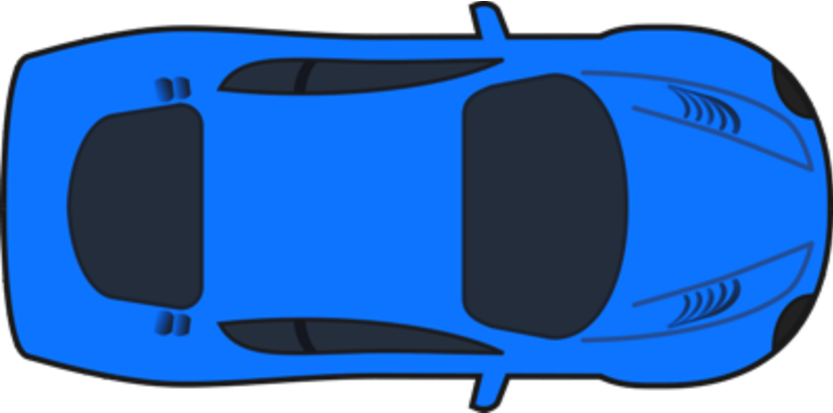
\includegraphics[scale=0.1]{blue_car.pdf}};
			\node (red1) [above left = -1.25cm and -1.8cm of rect] {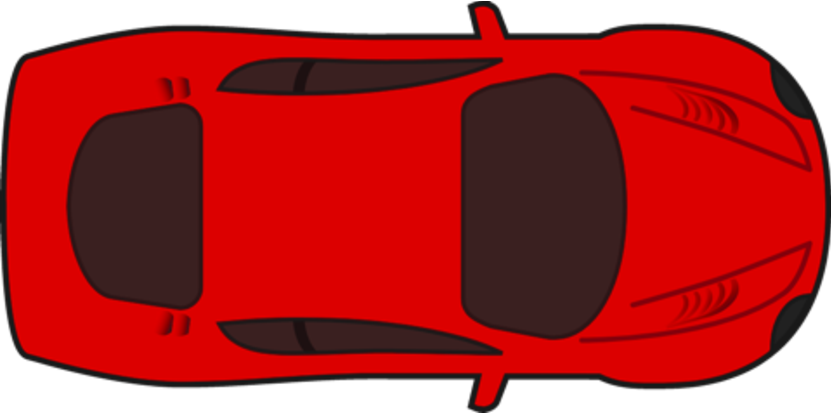
\includegraphics[scale=0.1]{red_car.pdf}};
			\node (red2)	[above right = -2.75cm and -2cm of rect]{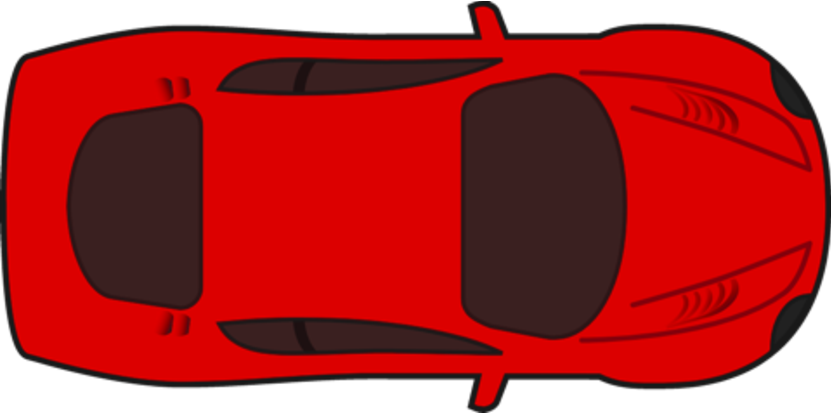
\includegraphics[scale=0.1]{red_car.pdf}};
			
			\node (mid3)	[above left = -1.58cm and -5.9cm of rect, minimum width = 0cm, minimum height = 0cm, inner sep = 0pt] {};
			\node (mid2)	[above left = -1.56cm and -4.9cm of rect, minimum width = 0.cm, minimum height = 0.cm, inner sep = 0pt] {};
			\node (mid1)	[above left = -1.56cm and -3.9cm of rect, minimum width = 0.cm, minimum height = 0.cm, inner sep = 0pt] {};
			
			
			
			
			\node (off_road_north) [draw = none, very thick, fill = black!60!green, minimum width = 8.25cm, minimum height = 1cm, inner sep = 0pt, above  = 0mm of rect, fill opacity=0.6] {};
			
			\node (off_road_south) [draw = none, very thick, fill = black!60!green, minimum width = 8.25cm, minimum height = 1cm, inner sep = 0pt, below  = 0mm of rect, fill opacity=0.6] {};
			
			
			\node (final)	[draw, circle, above right = -0.83cm and -0.5cm of rect, minimum width = 0.cm, minimum height = 0.cm, inner sep = 0pt] {};
			
			\node (final3)	[draw,  above right = -0.83cm and -1.5cm of rect, minimum width = 0.cm, minimum height = 0.cm, inner sep = 0pt] {};
			\node (final2)	[draw, circle, above right = -0.83cm and -2.5cm of rect, minimum width = 0.cm, minimum height = 0.cm, inner sep = 0pt] {};
			\node (final1)	[draw, circle, above right = -0.83cm and -3.5cm of rect, minimum width = 0.cm, minimum height = 0.cm, inner sep = 0pt] {};
			
			
			\node (breakaway1)	[draw, circle,  below left = -0.83cm and -3cm of rect, minimum width = 0.cm, minimum height = 0cm, inner sep = 0pt]{};
			\node (breakaway2)	[draw, circle,  below left = -0.83cm and -4cm of rect, minimum width = 0.cm, minimum height = 0cm, inner sep = 0pt]{};
			\node (breakaway3)	[draw, circle,  below left = -0.83cm and -5cm of rect, minimum width = 0.cm, minimum height = 0cm, inner sep = 0pt]{};		
			
			\draw [rounded corners,color=cyan,line width=3pt] (blue) .. controls (breakaway1) ..  (mid1) .. controls (final1) .. (final2) -- (final);
			\draw [rounded corners,color=line1,line width=3pt] (blue) .. controls (breakaway2) ..  (mid2) .. controls (final2) .. (final3) -- (final);
			\draw [rounded corners,color=line2,line width=3pt] (blue) .. controls (breakaway3) ..  (mid3) .. controls (final3) .. (final) ;

			\node [draw, fill = none, minimum width = 1.5cm, minimum height = 0.75cm, inner sep = 0pt, below left = -2.32cm and -1.19cm of blue, thin, dash dot, color = red] {};
		
			\node [draw, fill = none, minimum width = 1.5cm, minimum height = 0.75cm, inner sep = 0pt, below left = -0.86cm and -1.57cm of red2, thin, dash dot, color = red] {};
			
			\node [draw, fill = none, minimum width = 1.5cm, minimum height = 0.75cm, inner sep = 0pt, below left = -0.86cm and -1.57cm of blue, thin, dash dot, color = blue] {};
			
			\node[above left = -1.15cm and -2cm of blue,]{A};
			\node[above left = -1.15cm and -2.75cm of blue,]{A1};
			\node[above left = -1.15cm and -3.75cm of blue,]{A2};
			\node[above left = -1.15cm and -4.75cm of blue,]{A3};
			%		
			\node[above left = 1.15cm and -4.5cm of blue,]{B1};
			\node[above left = 1.15cm and -5.5cm of blue,]{B2};
			\node[above left = 1.15cm and -6.5cm of blue,]{B3};
			\node[above left = 1.15cm and -7.5cm of blue,]{B};
			
			\end{tikzpicture}
			\par
		\end{centering}
	\protect\caption{Possible lane changing sequences that can be chosen by the autonomous vehicle (blue) based on the motion of other non-autonomous vehicles (red) are $\left\{\left(A,A1\right),\,\left(A1,B1\right),\,\left(B1,B\right)\right\}$, $\left\{\left(A,A2\right),\,\left(A2,B2\right),\,\left(B2,B\right)\right\}$ and $\left\{\left(A,A3\right),\,\left(A3,B3\right),\,\left(B3,B\right)\right\}$.}
	\label{fig:lane_changing}
	\end{figure}
	
	
	%==========================================================================%

	\section{Vehicle dynamic model}
	\label{sec:model}

	The  vehicle dynamics are represented by the following discrete model \cite{Kong2015}
	\begin{subequations}
		\begin{align}
			x\left(t+1\right) & = 	x\left(t\right) + v\left(t\right) \cos\left(\psi \left(t\right) + \beta \left(t\right) \right) \Delta t + w_x\left(t\right)\\ 
			y\left(t+1\right) & = 	y\left(t\right) + v\left(t\right) \sin\left(\psi \left(t\right) + \beta \left(t\right) \right) \Delta t + w_y\left(t\right) \\ 
			\psi\left(t+1\right) & = 	\psi\left(t\right) + \frac{v\left(t\right)}{l_r} \sin\left( \beta \left(t\right) \right) \Delta t \\ 
			v\left(t+1\right) & = 	v\left(t\right) + a\left(t\right)  \Delta t\\
			\beta\left(t\right) & = \arctan\left(\frac{l_r}{l_r+l_f}\tan\left(\delta_f\left(t\right)\right)\right),
		\end{align}
	\label{eq:mod}
	\end{subequations}


	\noindent where  $t$ denotes the discrete time instant; the pair $\left(x\left(t\right),\,y\left(t\right)\right)$  represent the global position of the center of mass of the vehicle; the vehicle's speed is denoted by $v\left(t\right)$; 	$\beta\left(t\right)$ is the angle of $v\left(t\right)$ with respect to the longitudinal axis of the vehicle; $\psi\left(t\right)$ denotes the vehicle’s yaw angle (the angle between the vehicle’s heading direction and the global x-direction); $a\left(t\right)$ denotes the vehicle’s acceleration at time $t$;  $\Delta t$ denotes the time step size; $\delta_f\left(t\right)$  represents the front steering angle; and  $l_f$  and $l_r$  are the distance of the center of the mass of the vehicle to the front and rear axles, respectively; $w_x\left(t\right)$  and $w_x\left(t\right)$ denote the uncertainty in the position of the center of mass, respectively. It is assumed the uncertainties originate from a closed and compact disturbance set defined as 
	\begin{align}
		{\mathcal{W}} \coloneqq  \left\{ w = \left(w_x,\,w_y\right) |\zeta w\leq\theta,\,\zeta\in\mathbb{R}^{a\times 2},\,\theta\in\mathbb{R}^{b}\right\},
		\label{eq:dist_set}
	\end{align}
	where $b \in 2\mathbb{Z}^{+}$. The disturbance set is assumed to contain the origin. Furthermore, it is assumed that the rear wheels cannot be steered. Therefore, the control input to the model \eqref{eq:mod}, represented by $\gamma\left(t\right) = \left(a\left(t\right),\, \delta_f\left(t\right)\right)$, is the acceleration and front steering angle pair. 

	
	%==========================================================================%

	
	\section{Robust game-theoretic decision making}
	\label{sec:controller}

	At each time instant, each vehicle selects an input pair from the finite action set, $ \boldsymbol{\Gamma} = \left\{\left(0,\, 0\right),\,\left(0,\, \delta_{f,\,\textrm{nom}}\right),\,\left(0,\, -\delta_{f,\,\textrm{nom}}\right),\,\left(a_{\textrm{nom}},\, 0\right),\,\left(-a_{\textrm{nom}},\, 0\right),\right.$ $\left.\left(a_{\max},\, 0\right),\,\left(-a_{\max},\, 0\right),\,\left(a_{\textrm{nom}},\, \delta_{f,\,\max}\right),\,\left(a_{\textrm{nom}},\, -\delta_{f,\,\max}\right)\right\}$, where $a_{\textrm{nom}}$, $\delta_{f,\,\textrm{nom}}$ and $a_{\max}$, $\delta_{f,\,\max}$ are the nominal and maximum acceleration, front steer angle, respectively. The inputs pairs in $ \boldsymbol{\Gamma}$ correspond to the actions, \{``maintain", ``turn slightly left", ``turn slightly right", ``accelerate", ``decelerate", ``maximum acceleration", ``maximum deceleration", ``turn left and accelerate", `` turn right and accelerate'' \}, respectively. The input pair to be applied at every time step is decided based on optimizing a reward function.
	


	\subsection{Reward function}
	\label{sec:reward_function}
	
	The decision making process of the vehicle in choosing the optimal input pair follows a receding horizon strategy. The nominal model used within the prediction horizon is given by
	\begin{subequations}
		\begin{align}
			x_{t+j+1} & = 	x_{t+j} + v_{t+j} \cos\left(\psi_{t+j} + \beta_{t+j} \right) \Delta t \\ 
			y_{t+j+1} & = 	y_{t+j} + v_{t+j} \sin\left(\psi_{t+j} + \beta_{t+j} \right) \Delta t  \\ 
			\psi_{t+j+1} & = 	\psi_{t+j} + \frac{v_{t+j}}{l_r} \sin\left( \beta _{t+j} \right) \Delta t \label{eq:psi_pred}\\ 
			v_{t+j+1} & = 	v_{t+j} + a_{t+j}  \Delta t \label{eq:v_pred}\\
			\beta_{t+j} & = \arctan\left(\frac{l_r}{l_r+l_f}\tan\left(\delta_{f,\,{t+j}}\right)\right) \label{eq:beta_pred},
		\end{align}
	\label{eq:nom_mod}
	\end{subequations}

	\noindent where $j \in \mathbb{Z}_{\left[0,\,N-1\right]}$  represents the prediction step, and $\gamma_{t+j} = \left(a_{t+j},\, \delta_{f,\,t+j}\right)$ denotes the input pair applied to \eqref{eq:nom_mod} at a prediction step $j$. A sequence of actions, $\boldsymbol{\gamma_{t}} = \left\{\gamma_{t},\,\gamma_{t+1},\,\cdots,\,\gamma_{t+N-1}\right\}$, is chosen that maximizes a cumulative reward given by
	\begin{align}
	\mathcal{R}\left(\boldsymbol{\gamma_{t}}\right) = \sum_{j=0}^{N-1} \lambda^{j} R_{t+j},
	\label{eq:cum_reward}
	\end{align}
	
	\noindent where $R_{t+j}$ is the stage reward at a prediction step $j$ determined at time step $t$ for an input, $\gamma_{t+j} \in  \boldsymbol{\Gamma}$; $\lambda \in \left[0,\,1\right]$ is the discount factor. By the receding horizon strategy, the input applied to \eqref{eq:mod}, $\gamma\left(t\right)$, is the first element of $\boldsymbol{\gamma_{t}}^* = \left\{\gamma_{t}^*,\,\gamma_{t+1}^*,\,\cdots,\,\gamma_{t+N-1}^*\right\}$ is applied at each time instant $t$. The stage reward at a prediction step $j$, $R_{t+j}$, is defined as
	 \begin{align}
	 R_{t+j} = \boldsymbol{{\alpha}}^T \boldsymbol{\phi_{t+j}},
	 \label{eq:stage_reward}
	 \end{align}
	
	\noindent where $\boldsymbol{{\phi}_{t+j}} = \left\{\phi_{1,\,{t+j}},\,\phi_{2,\,{t+j}},\,\cdots,\,\phi_{m,\,{t+j}}\right\}$ is the feature vector at step $j$ and the weights for these features are in  $\boldsymbol{{\alpha}} = \left\{\alpha_{1},\,\alpha_{2},\,\cdots,\,\alpha_{m}\right\}$, in which $\alpha_{i}>0,\,\forall \, i\in \mathbb{Z}_{\left[0:m\right]}$. For the lane changing scenario in  Fig.~\ref{fig:lane_changing}, the  features considered are described below. 
	
	Rectangular outer approximation of the geometric contour of each vehicle is considered as shown by the dash-dotted boxes in Fig.~\ref{fig:lane_changing}. This outer approximation is referred as the collision avoidance zone (c). The features, $\phi_{1,\,{t}},\,\phi_{2,\,{t}}$ and $\phi_{3,\,{t}}$, are indicator functions based on the collision avoidance zone of the vehicles that respectively characterize:
	\begin{itemize}
		\item Collision status - The intersection of the collision avoidance zone of the ego vehicle with that of any other vehicle indicates a collision or a danger of collision. If an overlap is detected then $\phi_{1,\,{t}}$ is assigned a value $-1$; and $0$, otherwise.
		
		\item On-road status - The intersection of the collision avoidance zone of the ego vehicle with that of green regions shown in Fig.~\ref{fig:lane_changing} indicates that the ego vehicle is outside the road boundaries. The feature $\phi_{2,\,{t}} = -1$ if an overlap is detected; $\phi_{2,\,{t}} = 0$, otherwise.
		
		\item Safe zone violation status - A safe zone (s) of a vehicle is a rectangular area that subsumes the collision avoidance zone of the vehicles with a safety margin. The safety margin is chosen based on the minimum distance to be maintained from the surrounding vehicles. If an overlap of the safe zone of the ego vehicle with that of another vehicle is detected then $\phi_{3,\,{t}}$ is assigned a value $-1$; and $0$, otherwise.		
		
		
	\end{itemize}
	 
	The other features considered in this work characterize:
	\begin{itemize}
	 	\item Distance to objective - In order to encourage the ego vehicle to change lane and reach a reference point in the new lane, $\left(x^{\textrm{ref}},\,y^{\textrm{ref}}\right)$, the feature $\phi_{4,\,{t}} $ is defined as
	 	\begin{align}
	 		\phi_{4,\,{t}}  = -\left(\left|x_{t}-x^{\textrm{ref}}\right| + \left|y_{t}-y^{\textrm{ref}}\right|\right).
	 	\end{align}
	 	
	 	\item Distance to lane center - The feature, $\phi_{5,\,{t}} $, defined as 
	 	 \begin{align}
	 	 \phi_{5,\,{t}}  = - \left|y_{t}-y^{lc}\right|,
	 	 \end{align}
	 	 
	 	 \noindent where $y^{lc}$ is the y-coordinate of the center of the current lane that is included to encourage the ego vehicle to be at the middle of the current lane.
	 	 
	 	\item Velocity error - The deviation of the velocity of the ego vehicle from a reference velocity, $v^{\textrm{ref}}$, is described by the feature $\phi_{6,\,{t}}$ as
	 	\begin{align}
	 		\phi_{6,\,{t}} = - \left|v_{t}-v^{\textrm{ref}}\right|,
	 	\end{align}
	 	where the reference velocity is typically chosen as the legislated speed limit.
	\end{itemize}
 


 
 	\subsection{Level-k framework}
	\label{sec:level_k}

	In a multi-agent traffic scenario, the interactive nature of the decision making process is taken into account by the features, $\phi_{1,\,t}$ and $\phi_{3,\,t}$, of the stage reward in \eqref{eq:stage_reward} that depend on the states of other vehicles. To compute the cumulative reward in \eqref{eq:cum_reward}, for a given sequence of actions of the \nth{l} autonomous vehicle, $\actseq{l}$, it is required to predict the actions of other agents, $\actseq{i}$, $\forall i \in \mathcal{O}$, where $\mathcal{O}=\left\{i|i \in \mathbb{Z}_{\left[1,\,n\right]},\, i\neq l \right\}$ with $n$ representing the number of agents, and the corresponding state of the traffic, $s_{t+j}$,  at prediction steps $j=0,\,1,\,\cdots,\,N-1$, where $s_t = \left[x_t{\left[1\right]},\,y_t{\left[1\right]},\,v_t{\left[1\right]},\,\theta_t{\left[1\right]},\,\cdots,\,x_t{\left[n\right]},\,y_t{\left[n\right]},\,v_t{\left[n\right]},\,\theta_t{\left[n\right]}\right]^T$. In this paper, level-k game theory \cite{Costa-Gomes2006,Costa-Gomes2009} is utilized to model the vehicle-to-vehicle interactions and thus predict the actions of the other agents over the horizon.

	In level-$k$ game theory, it is assumed that the decisions taken by the strategic agents are based on the predictions of the actions of the other agents and the agents can have have different reasoning levels. The reasoning depth of an agent is indicated by $k \in \left\{0,\,1,\,\cdots\right\}$. The hierarchy begins with agents at level-0, where the agents make instinctive decisions to achieve the objective without accounting for the interactions between other agents. On the other hand, the agents at level-$k$ $\forall k>0$, consider the interactions by assuming that the other agents are at level-$(k-1)$ and take decisions accordingly. For instance, a \nth{l} level-1 agent assumes other agents are at level-0 and predicts their action sequences, $\actseqk{i}{0}$ $\forall i \in \mathcal{O}$, to compute its own action sequence, $\actseqk{l}{1}$.
	
	The level-k game theory was adapted to model the vehicle-to-vehicle interactions at an unsignalized four-way intersection in \cite{Li2018}. It is assumed that level-0 vehicles consider the other vehicles in the traffic scenario as stationary obstacles. Therefore, these level-0 drivers implicitly assume the others will yield the right of way, and can be regarded `aggressive'. And level-1 drivers consider other drivers to be aggressive and take `cautious' actions. In \cite{Li2018}, the drivers are categorized into level-0, 1 and 2. Since, the behavior of level-2 driver will be similar to that of the level-0 drivers, in this paper, only level-0 and 1 drivers are considered. The stage reward value obtained for \nth{l} level-$k$ agent at a prediction step $j$ for an action $\actk{l}{k}{t+j}$, depend on the current traffic state, $s_0$, the ego agent's actions, $\actseqkt{l}{k}{j-1}$, and the actions of other agents, $\actseqkt{i}{k-1}{j-1}$ $\forall i \in \mathcal{O}$, is given as
	\begin{align}
		R_{t+j}^{(k)}[l] = R_{t+j} & \left( \actk{l}{k}{t+j}  \left| s_0,\, \actseqktnopar{l}{k}{j-1},\right.\right. \nonumber\\
		& \hspace{0.25cm} \left.\,\actseqktnopar{i}{k-1}{j-1}\right),
		\label{eq:stage_reward_multi}
	\end{align}
	
	\noindent and its cumulative reward is
	\begin{align}
		\mathcal{R}^{(k)}\left(\boldsymbol{\gamma_{t}^{(k)}[l]}\right) = \sum_{j=0}^{N-1} \lambda^{j} R_{t+j}^{(k)}[l].
		\label{eq:cum_reward_multi}
	\end{align}


	\subsection{Multi-model strategy}

	Human drivers, initially, do not have perfect knowledge about other drivers. However, they gain better understandings of other driver's characteristics through interactions, and therefore, resolve conflicts effectively. Similarly, the autonomous vehicles in a multi-agent traffic scenario, hold an initial belief about the driver model (level-0 and 1) of the other vehicles as a probability distribution over both models. Subsequently, based on the actual action applied by the other agents, the estimate of the probability distribution is updated at every step.
	
	From the perspective of an \nth{l} autonomous agent, the probability that the \nth{i} other agent can be modeled as level-$k$ is represented by $P_{K_{i}^l = k}$. The probability of the model $k$ is increased when it matches the actual action by 
	\begin{subequations} \label{lv_est}
		\begin{align}
			&k^* = \arg \, \underset{k \in \left\{0,\,1 \right\}} {\min} \left\| \actt{i}{k}{t} - \actk{i}{k}{t}  \right\|  \\ 
			& \tilde{P}_{K_{i}^l = k^*} \left(t\right) = {P}_{K_{i}^l = k^*} \left(t-1\right) + \Delta P  \\ 
			& {P}_{K_{i}^l = k}\left(t\right) = \frac{\tilde{P}_{K_{i}^l = k}\left(t\right) }{\sum_{\tilde{k} = 0}^{1} \tilde{P}_{K_{i}^l = \tilde{k}}\left(t\right) },  \forall k \in \left\{0,\,1 \right\},
		\end{align}
		\label{eq:model_update}
	\end{subequations}
	
	\noindent where $\actt{i}{k}{t}$ and $\actk{i}{k}{t}$ represent the actual and predicted action taken by \nth{i} agent assuming level-$k$ model, respectively; $\Delta P >0 $ is a constant that denotes the rate of increment of the probability;  $\left\|\actt{i}{k}{t} - \actk{i}{k}{t}\right\| = \left| a\left(t\right) - a_t^{(k)} \right| + \left|  \delta_f\left(t\right) - \delta_{f,\,t}^{(k)} \right|$. When the input pair of the actual action is equal to that of the predicted action, the probability distribution remains unchanged.

	
	In order to incorporate the multi-model strategy in the decision making process and select the optimal action according to the model of other agents, the expected cumulative reward for the \nth{l} agent, using \eqref{eq:stage_reward_multi} and \eqref{eq:cum_reward_multi}, is given by
	\begin{align}
		\mathcal{R}_P\left(\boldsymbol{\gamma_{t}}[l]\right)  = \sum_{k=0}^{1} {P}_{K_{i}^l = k}\left(t\right)  \mathcal{R}^{(k)}\left(\boldsymbol{\gamma_{t}^{(k)}}[l]\right),\, \forall i \in \mathcal{O}.
		\label{eq:cum_reward_prob}
	\end{align}
	 


	\subsection{Robust decision making}
	\label{sec:robust}

	The mismatch between the actual position of the center of mass of the vehicle which is used to determine the rectangular outer approximation of the vehicle (see Section \ref{sec:reward_function}) and its predictions obtained using the dynamic model in \eqref{eq:nom_mod} might lead to collision. In the multi-agent traffic scenario under consideration, there are two sources of modeling errors: (i) the uncertainties, $w^{(m)} = \left(w_x^{(m)},\,w_y^{(m)}\right) \in \mathcal{W}_m$, resulting due to the use of a simplified model in \eqref{eq:nom_mod}; and (ii) the uncertainty, $w^{(d)} = \left(w_x^{(d)},\,w_y^{(d)}\right) \in \mathcal{W}_d$, arising due to unknown driver model. Hence, the disturbance set defined in \eqref{eq:dist_set} is 
	\begin{align}
		\mathcal{W} = \mathcal{W}_m \oplus \mathcal{W}_d.
		\label{eq:full_dist_set}	
	\end{align}
	 	
	
	
	Robust approaches can be used to account for these uncertainties while computing the control actions. Since a discrete set of input actions is considered in this work, feedback min-max strategy \cite{Scokaert1998} is utilized in this work for considering the uncertainties originating from the disturbance set $\mathcal{W}$. Since the autonomous agents update the driver models of the other agents in the multi-agent traffic scenario at each step according to \eqref{eq:model_update}, an adaptive scheme is proposed to incorporate the confidence on the driver models and leverage the fact that level-1 drivers are cautious. The disturbance set considered at each time step is modified  of the other agents and leverage .

	

	\begin{align}
		\bar{\mathcal{W}}_{i}^{l}(t) = \mathcal{W}_m \oplus P_{K_{i}^l = 0}(t) \mathcal{W}_d
		\label{eq:adaptive_dist_set}
	\end{align}

	\noindent where at time $t$, $P_{K_{i}^l = 0} (t) $ is the probability that the \nth{i} agent is a level-0 driver from the perspective of the \nth{l} autonomous agent, and $\bar{\mathcal{W}}_{i}^{l}(t)$ denotes the disturbance set. It is assumed that, initially, all the agents are level-0 drivers, i.e., $P_{K_{i}^l = 0} (0) = 1,\, \forall i \in \mathcal{O}$. Essentially, this assumption allows the autonomous agent to be cautious with another interacting agent when there is no/less information about that agent. If an \nth{i} agent is level-0, as time evolves, $P_{K_{i}^l = 0} (t)$ will continue to be equal to one, and hence, the autonomous agent take conservative actions (or behave like level-1 driver). On the other hand, when the \nth{i} agent is a level-1 driver, $P_{K_{i}^l = 0} (t)$ will decrease, resulting in a reduced disturbance set size, thereby, allowing the autonomous agent to take less conservative actions and adapt to the behavior of the interacting agents while capable of handling the uncertainties arising due to the use of a simple prediction model. 

	When interacting with an agent $i\in \mathcal{O}$, the objective the autonomous agent $l$ is to maximize the expected cumulative reward \eqref{eq:cum_reward_multi}, while accounting for the effect of the worst-case uncertainty from the possible disturbance realizations. The optimal control sequence, $\optactseq{l}$, is obtained by solving the following optimization problem
	\begin{subequations}
		\begin{align}
			\boldsymbol{\gamma^{*}_{t}[l]} =  & \arg \underset {\boldsymbol{\gamma_{t}[l]} \in  \boldsymbol{\Gamma}} {\max}\, \, \underset{w_{t+j}^{p} \in \bar{\mathcal{W}}_{i}^{l}(t)}{\min} \, \, \mathcal{R}_P\left(\boldsymbol{\gamma_{t}[l]}\right) \\
			\textrm{s. t.} \forall &  j \in \mathbb{Z}_{0,\,N-1},\, \eqref{eq:psi_pred},\, \eqref{eq:v_pred},\, \eqref{eq:beta_pred} ,\,\forall i \in \mathcal{O},\, \forall p \in \mathcal{P} \nonumber \\
			\tilde{x}_{t+j+1} & = 	\tilde{x}_{t+j} + v_{t+j} \cos\left(\psi_{t+j} + \beta_{t+j} \right) \Delta t + w_{x,\,t+j}^{p}\\ 
			\tilde{y}_{t+j+1} & = 	\tilde{y}_{t+j} + v_{t+j} \sin\left(\psi_{t+j} + \beta_{t+j} \right) \Delta t + w_{x,\,t+j}^{p},
			\label{eq:control_action_model}
		\end{align}
		\label{eq:control_prob}
	\end{subequations}

	
	\noindent where $w_{t+j}^{p} = \left(w_{x,\,t+j}^{p},\, w_{y,\,t+j}^{p}\right)$ denote a possible realization of the uncertainty in the global position of the center of mass in $x$ and $y$ directions, respectively; and $\mathcal{P}$ represents the set of indexes of the realizations. The autonomous agent then applies the first element $\optact{l}$ of the optimal control action sequence, i.e.,  $\gamma\left(t\right) = \optact{l}$.
	

	% This does not account for the confidence on the driver model
	
	% safe zone can be used to define the uncertainties in the vehicle dynamic model.. however we shd account for uncertainty in the driver model estimation
	
	\begin{figure*}
		\begin{centering}
			\begin{tikzpicture}[scale=0.4,transform shape]
			\node (origin) at (0,0) {};
			
			\node (adp1)[below left = 0cm and 0cm of origin, minimum width = 0.cm, minimum height = 0cm, inner sep = 0pt]{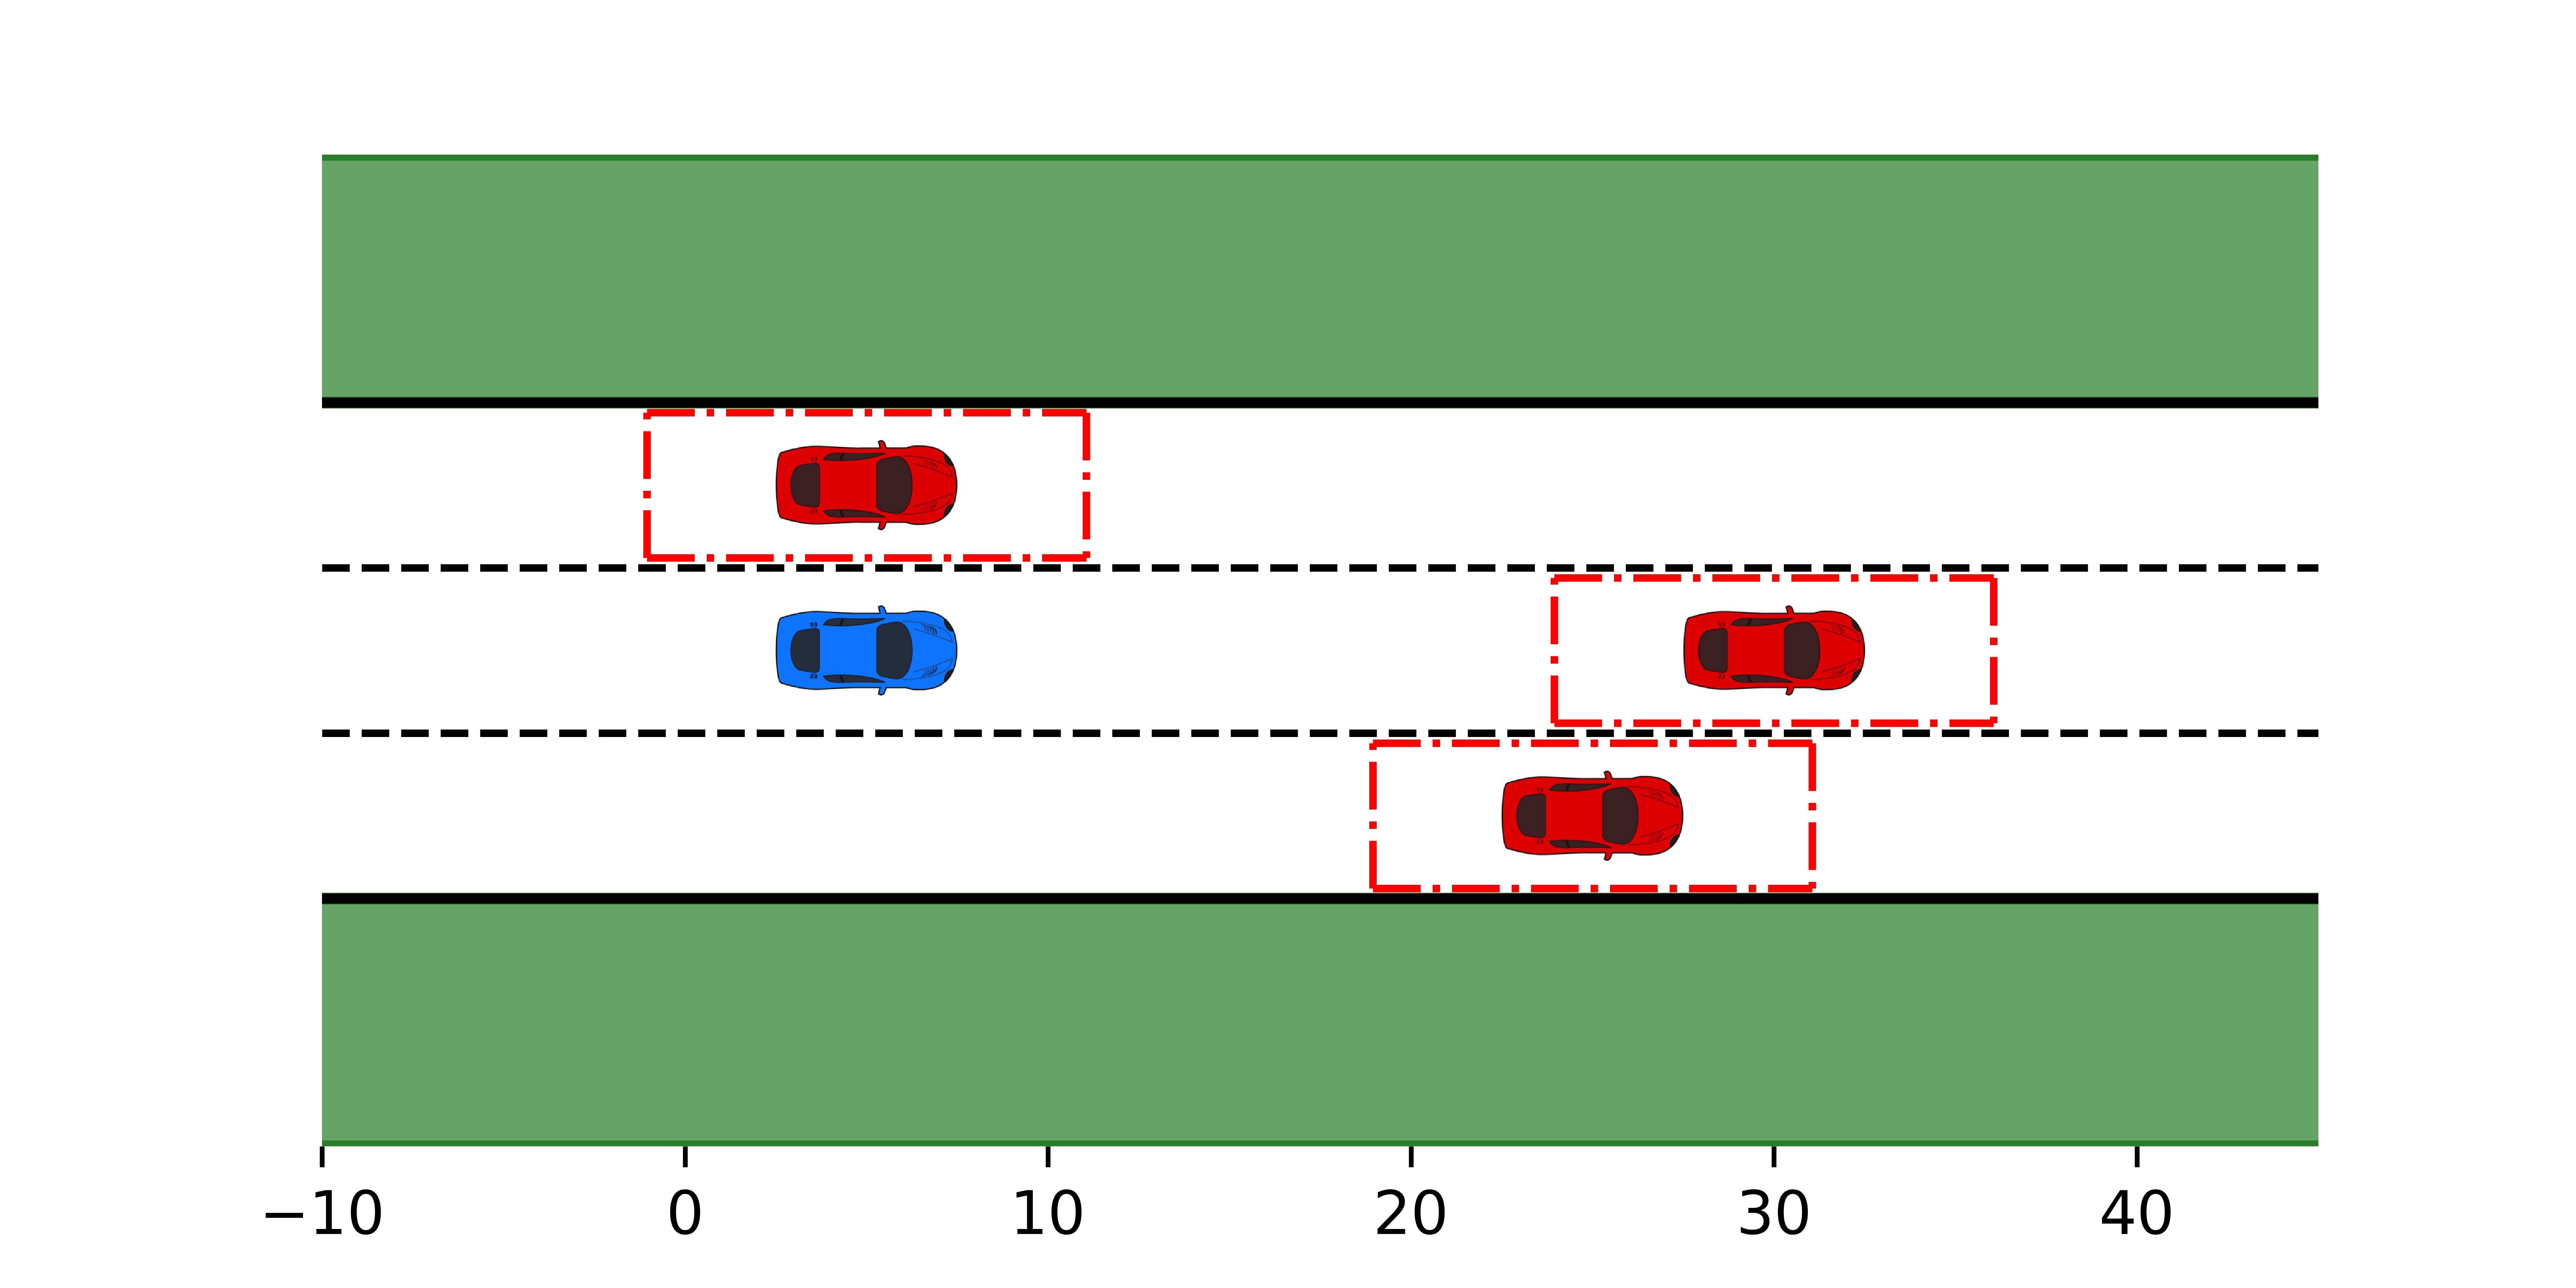
\includegraphics[clip, trim = {1.5cm 0.25cm 1.5cm 0.25cm}]{plot_adp0.jpg}};
			\node (agg1)[left = 1cm of adp1, minimum width = 0.cm, minimum height = 0cm, inner sep = 0pt]{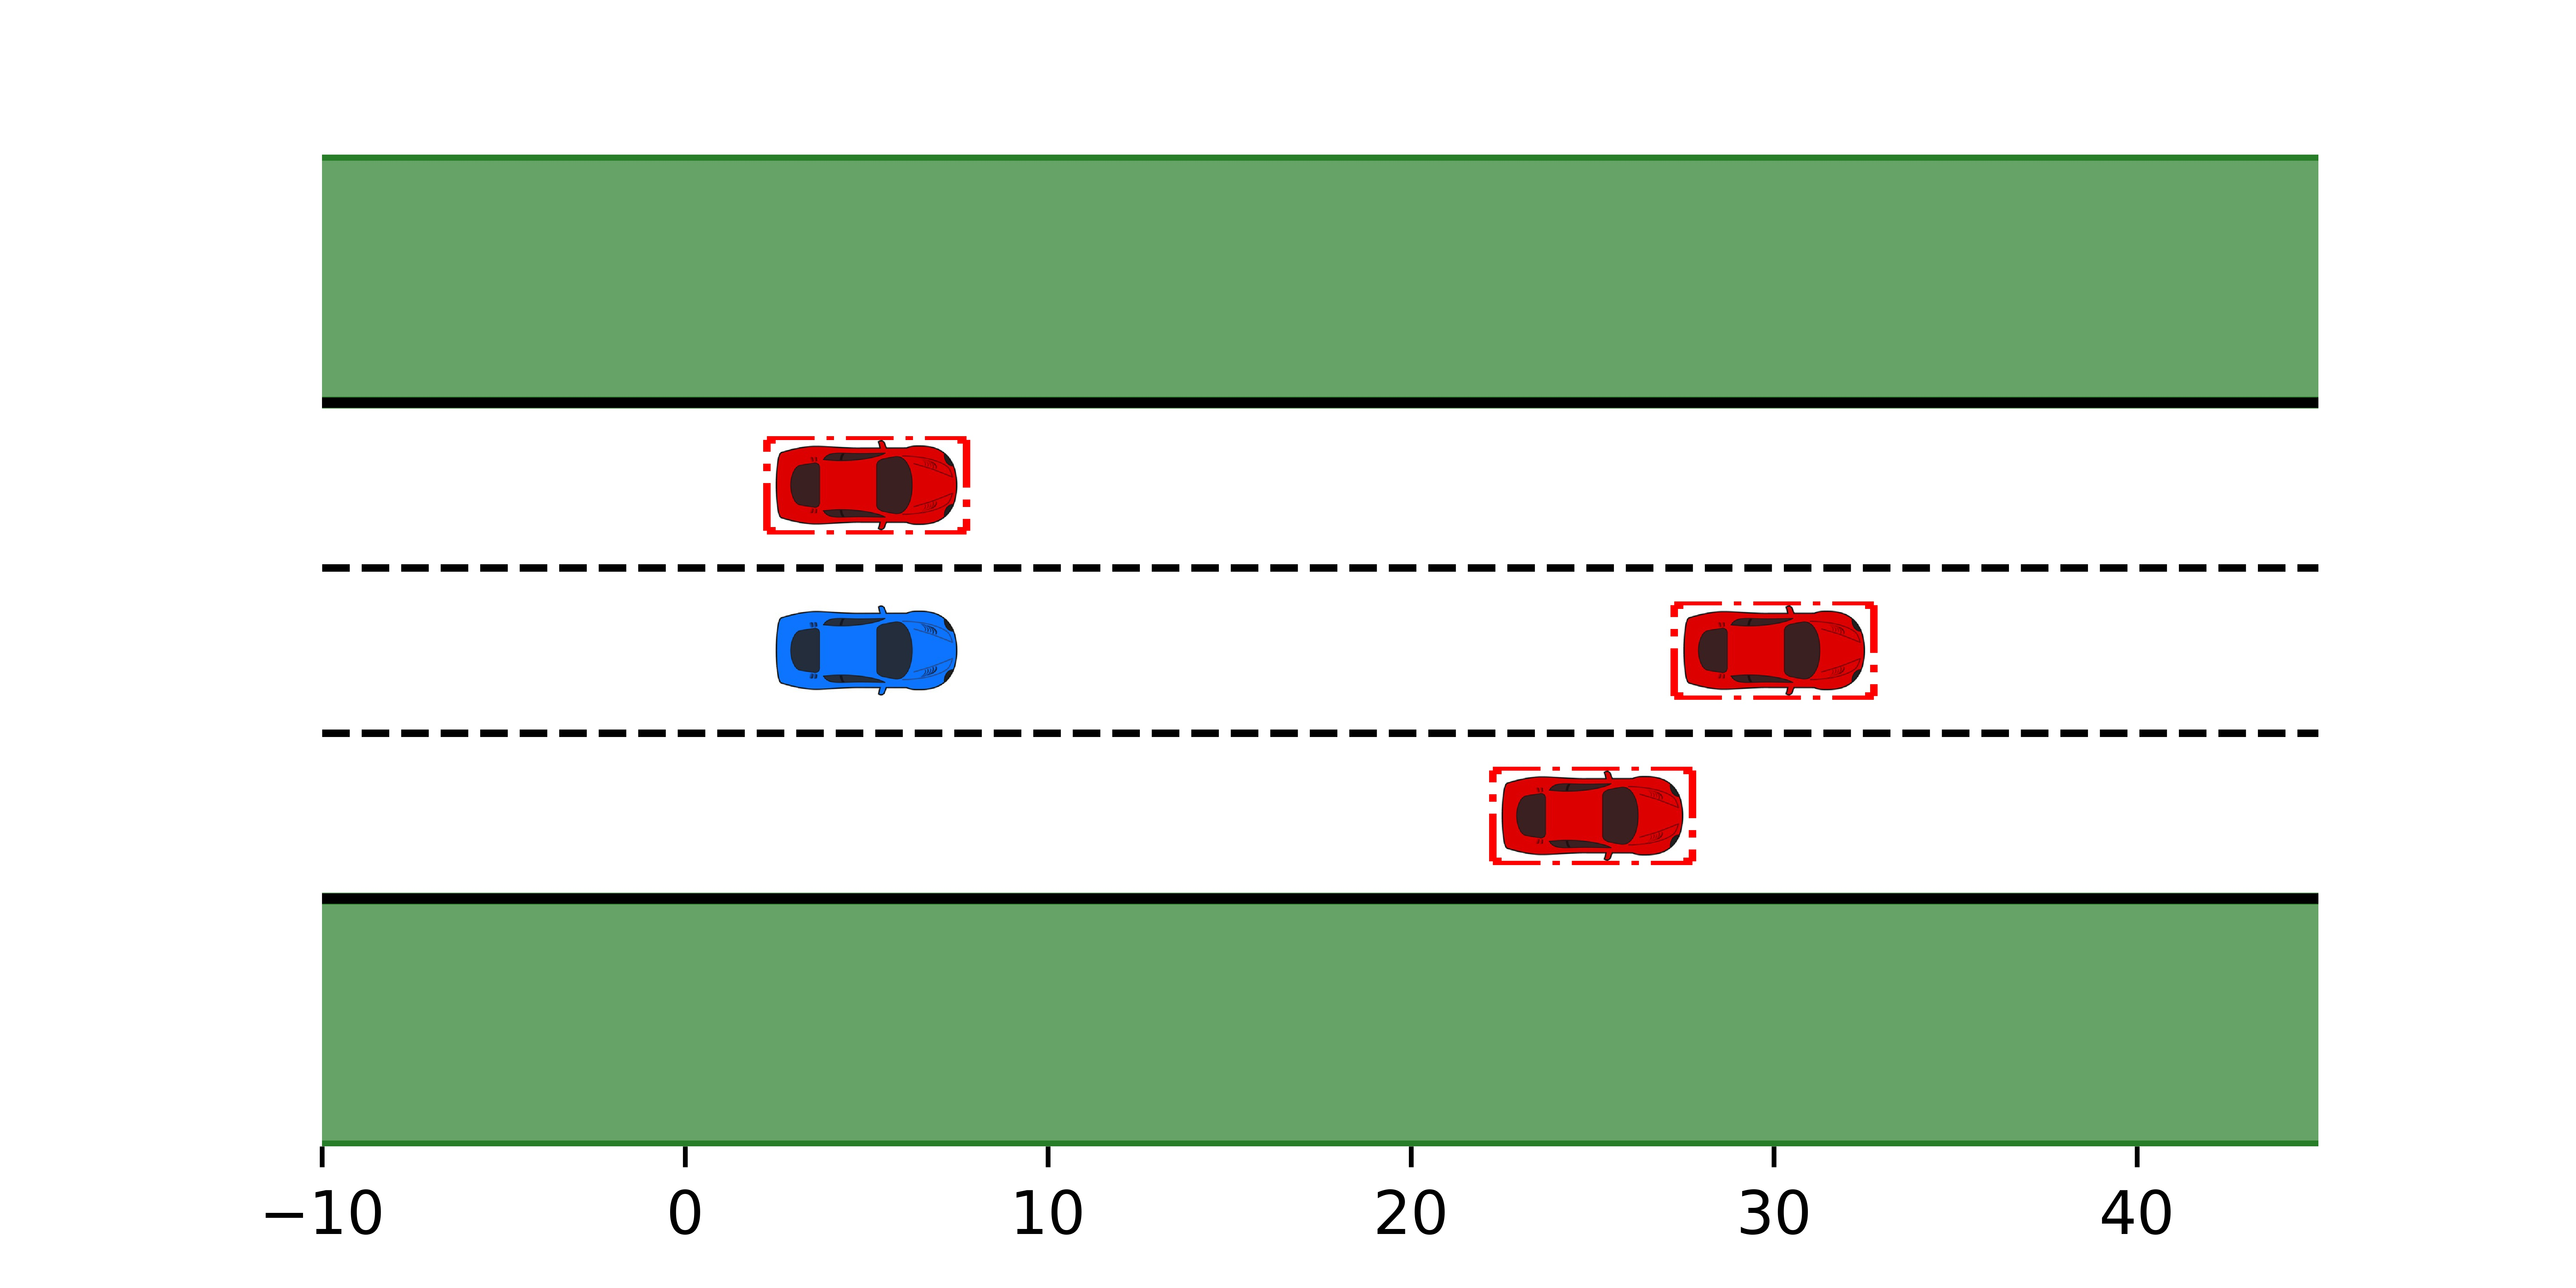
\includegraphics[clip, trim = {1.5cm 0.25cm 1.5cm 0.25cm}]{plot_agg0.jpg}};
			\node (con1)[ right = 1cm of adp1, minimum width = 0.cm, minimum height = 0cm, inner sep = 0pt]{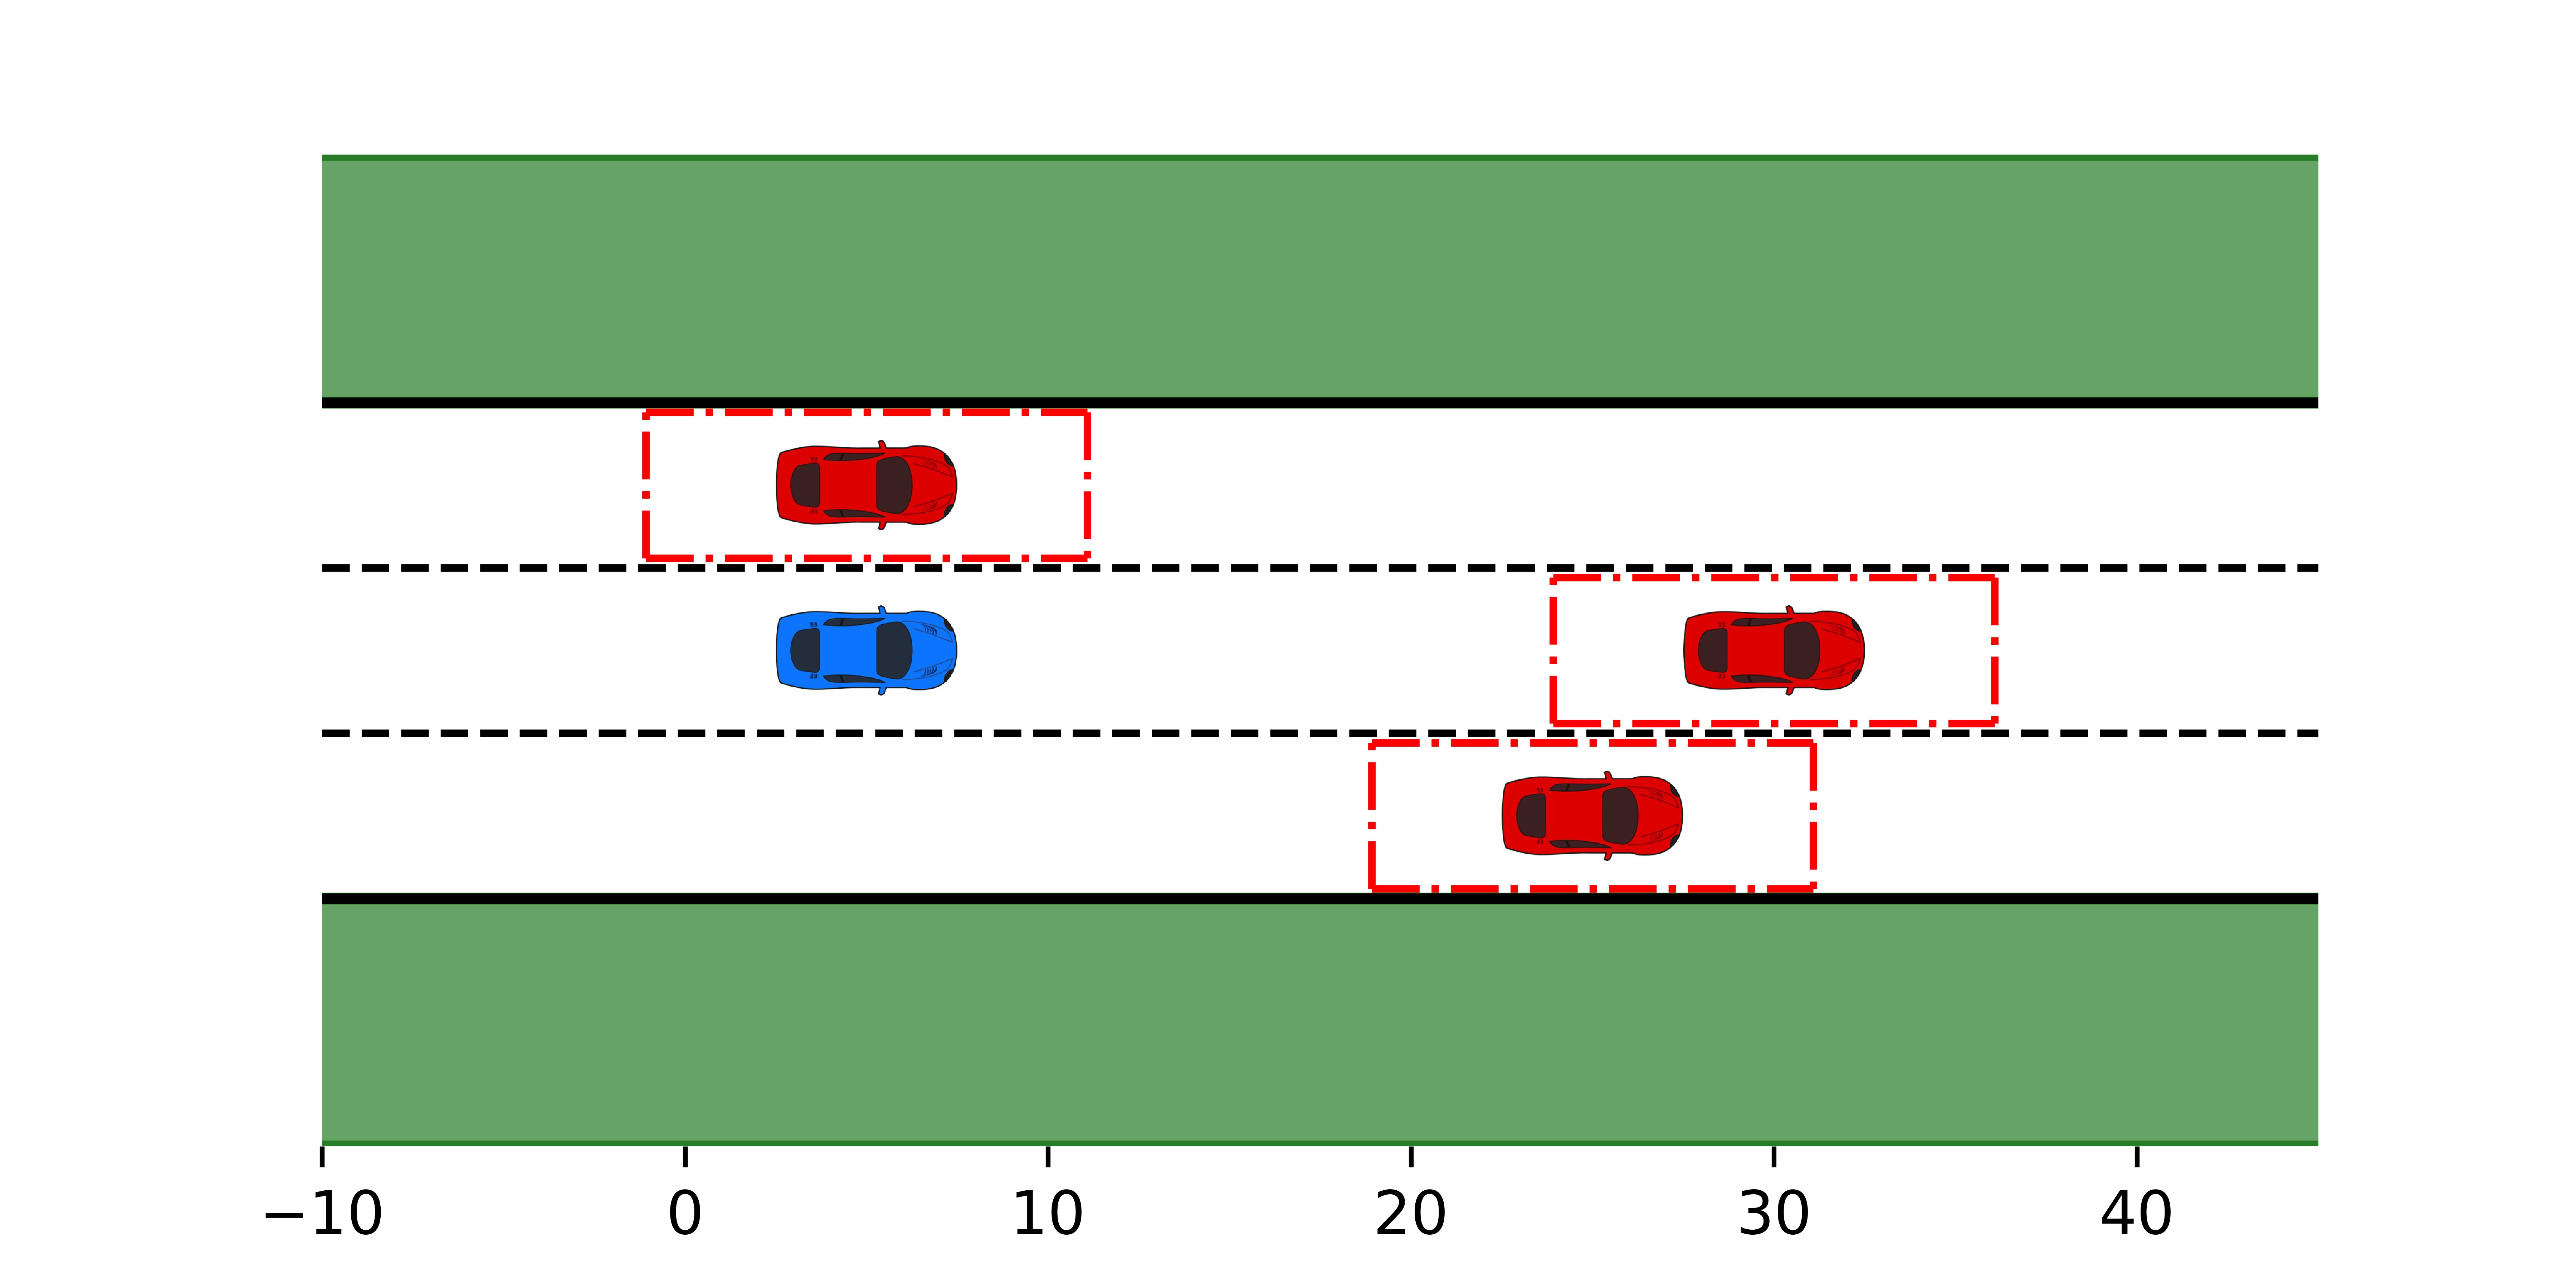
\includegraphics[clip, trim = {1.5cm 0.25cm 1.5cm 0.25cm}]{plot_con0.jpg}};
			
			
			\node (adp2)[below  = 1.cm of adp1, minimum width = 0.cm, minimum height = 0cm, inner sep = 0pt]{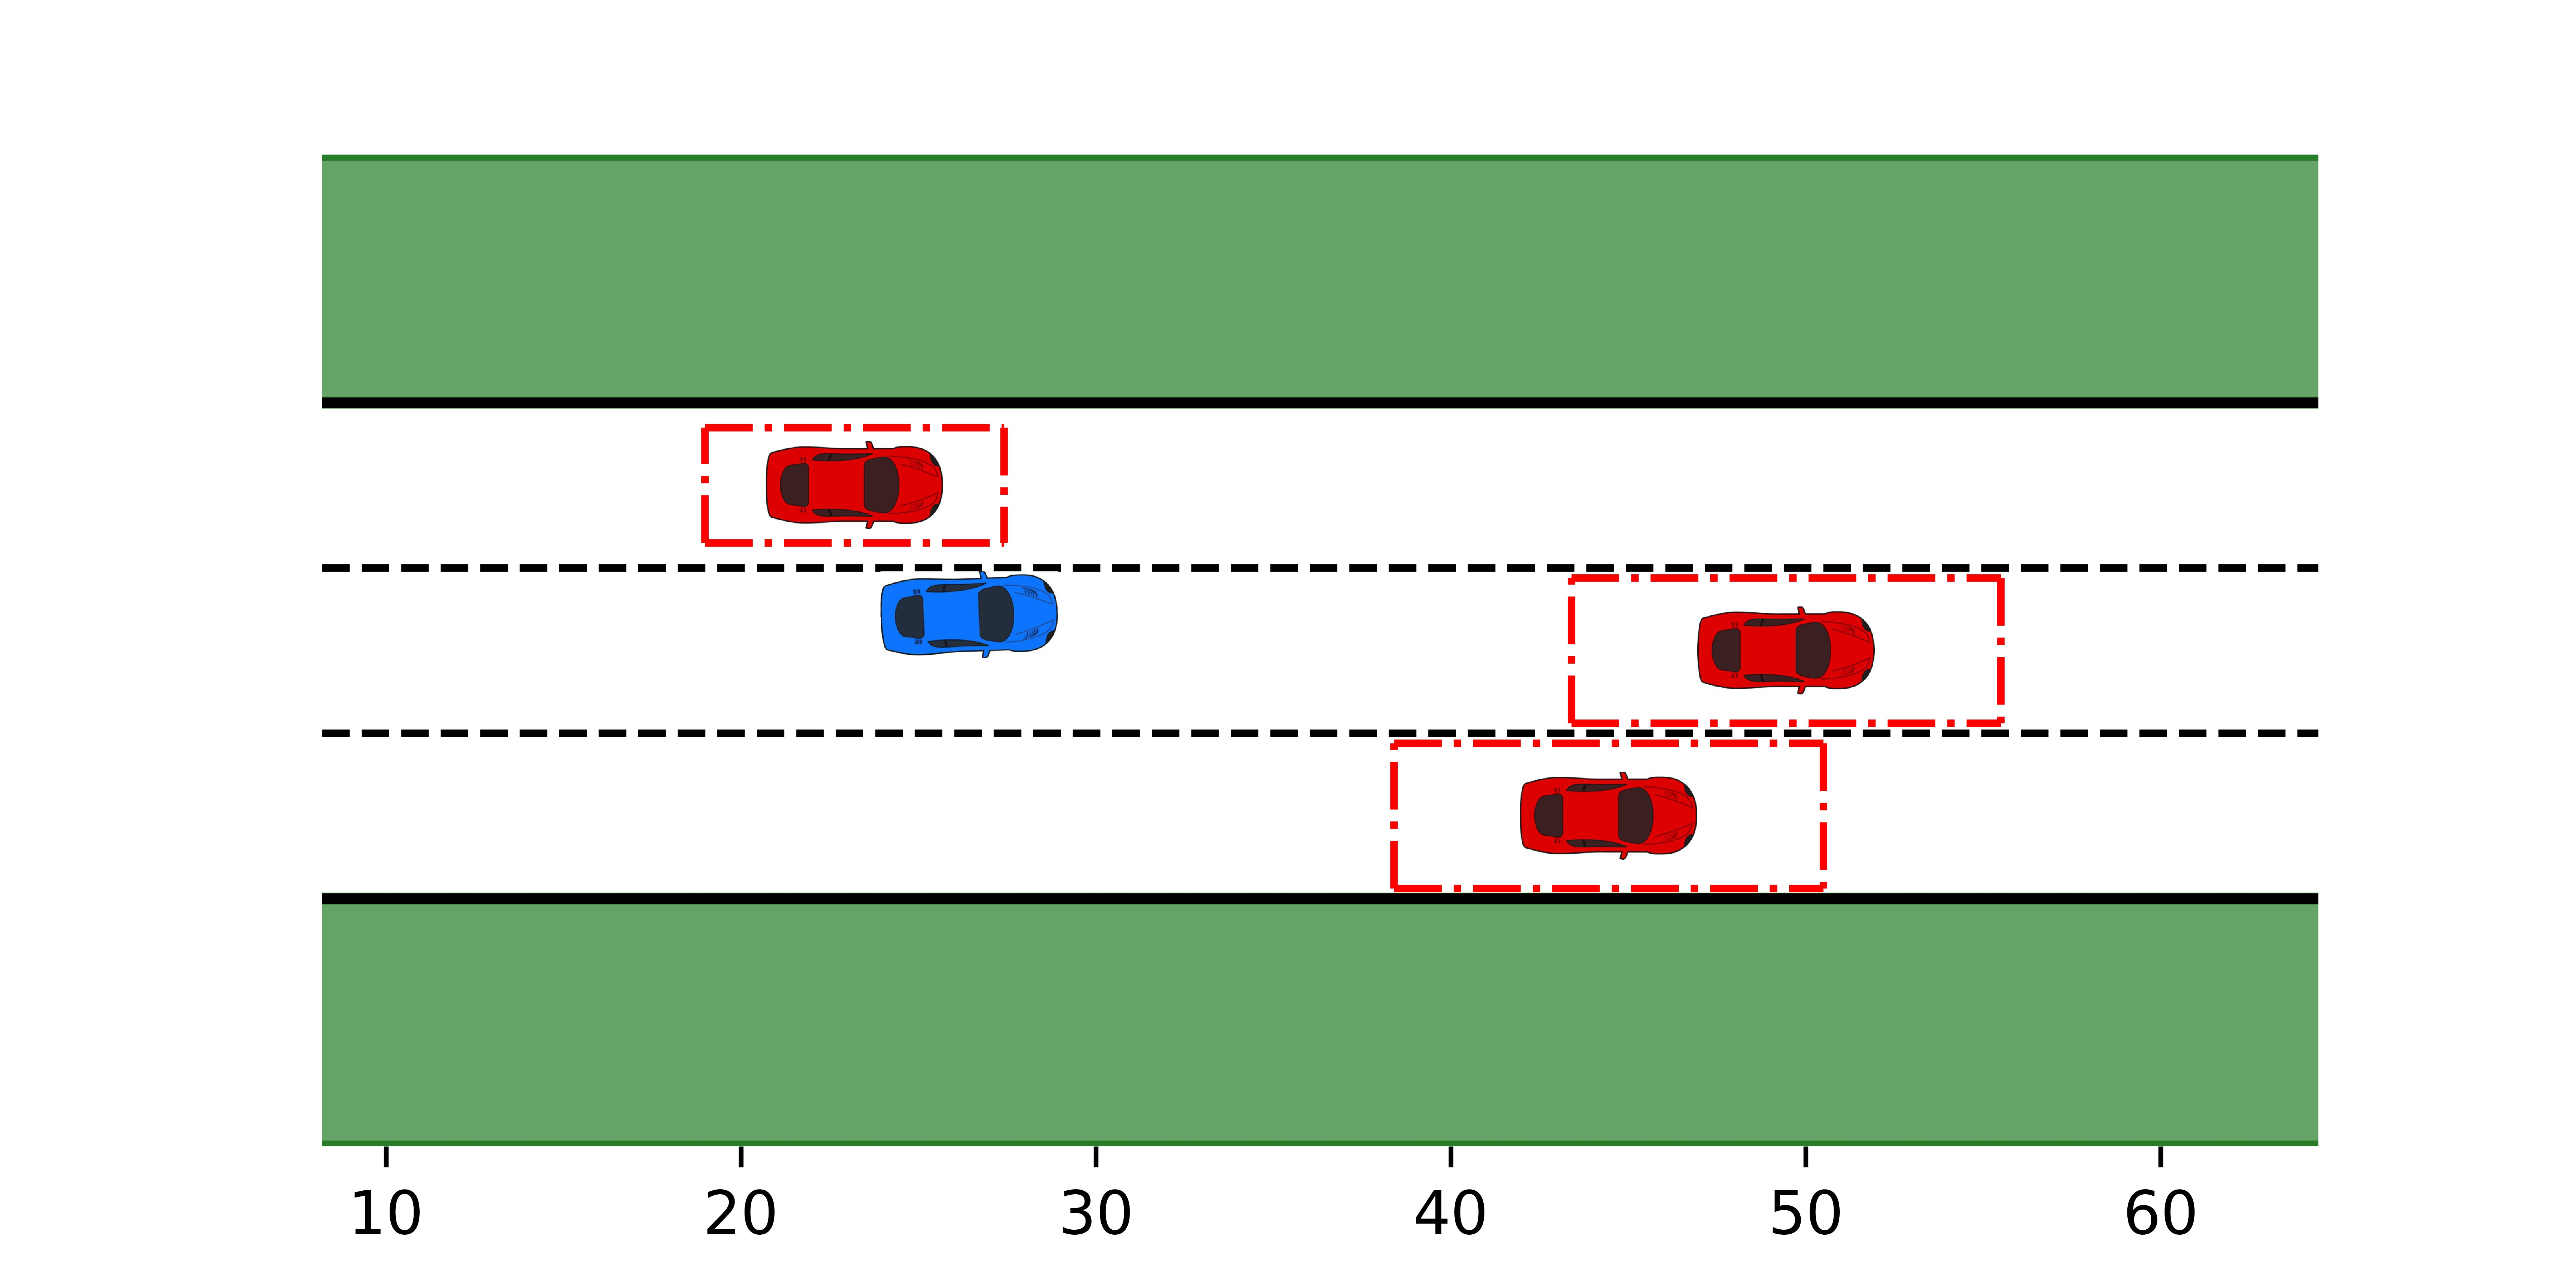
\includegraphics[clip, trim = {1.5cm 0.25cm 1.5cm 0.25cm}]{plot_adp2.jpg}};
			\node (agg2)[left = 1cm of adp2, minimum width = 0.cm, minimum height = 0cm, inner sep = 0pt]{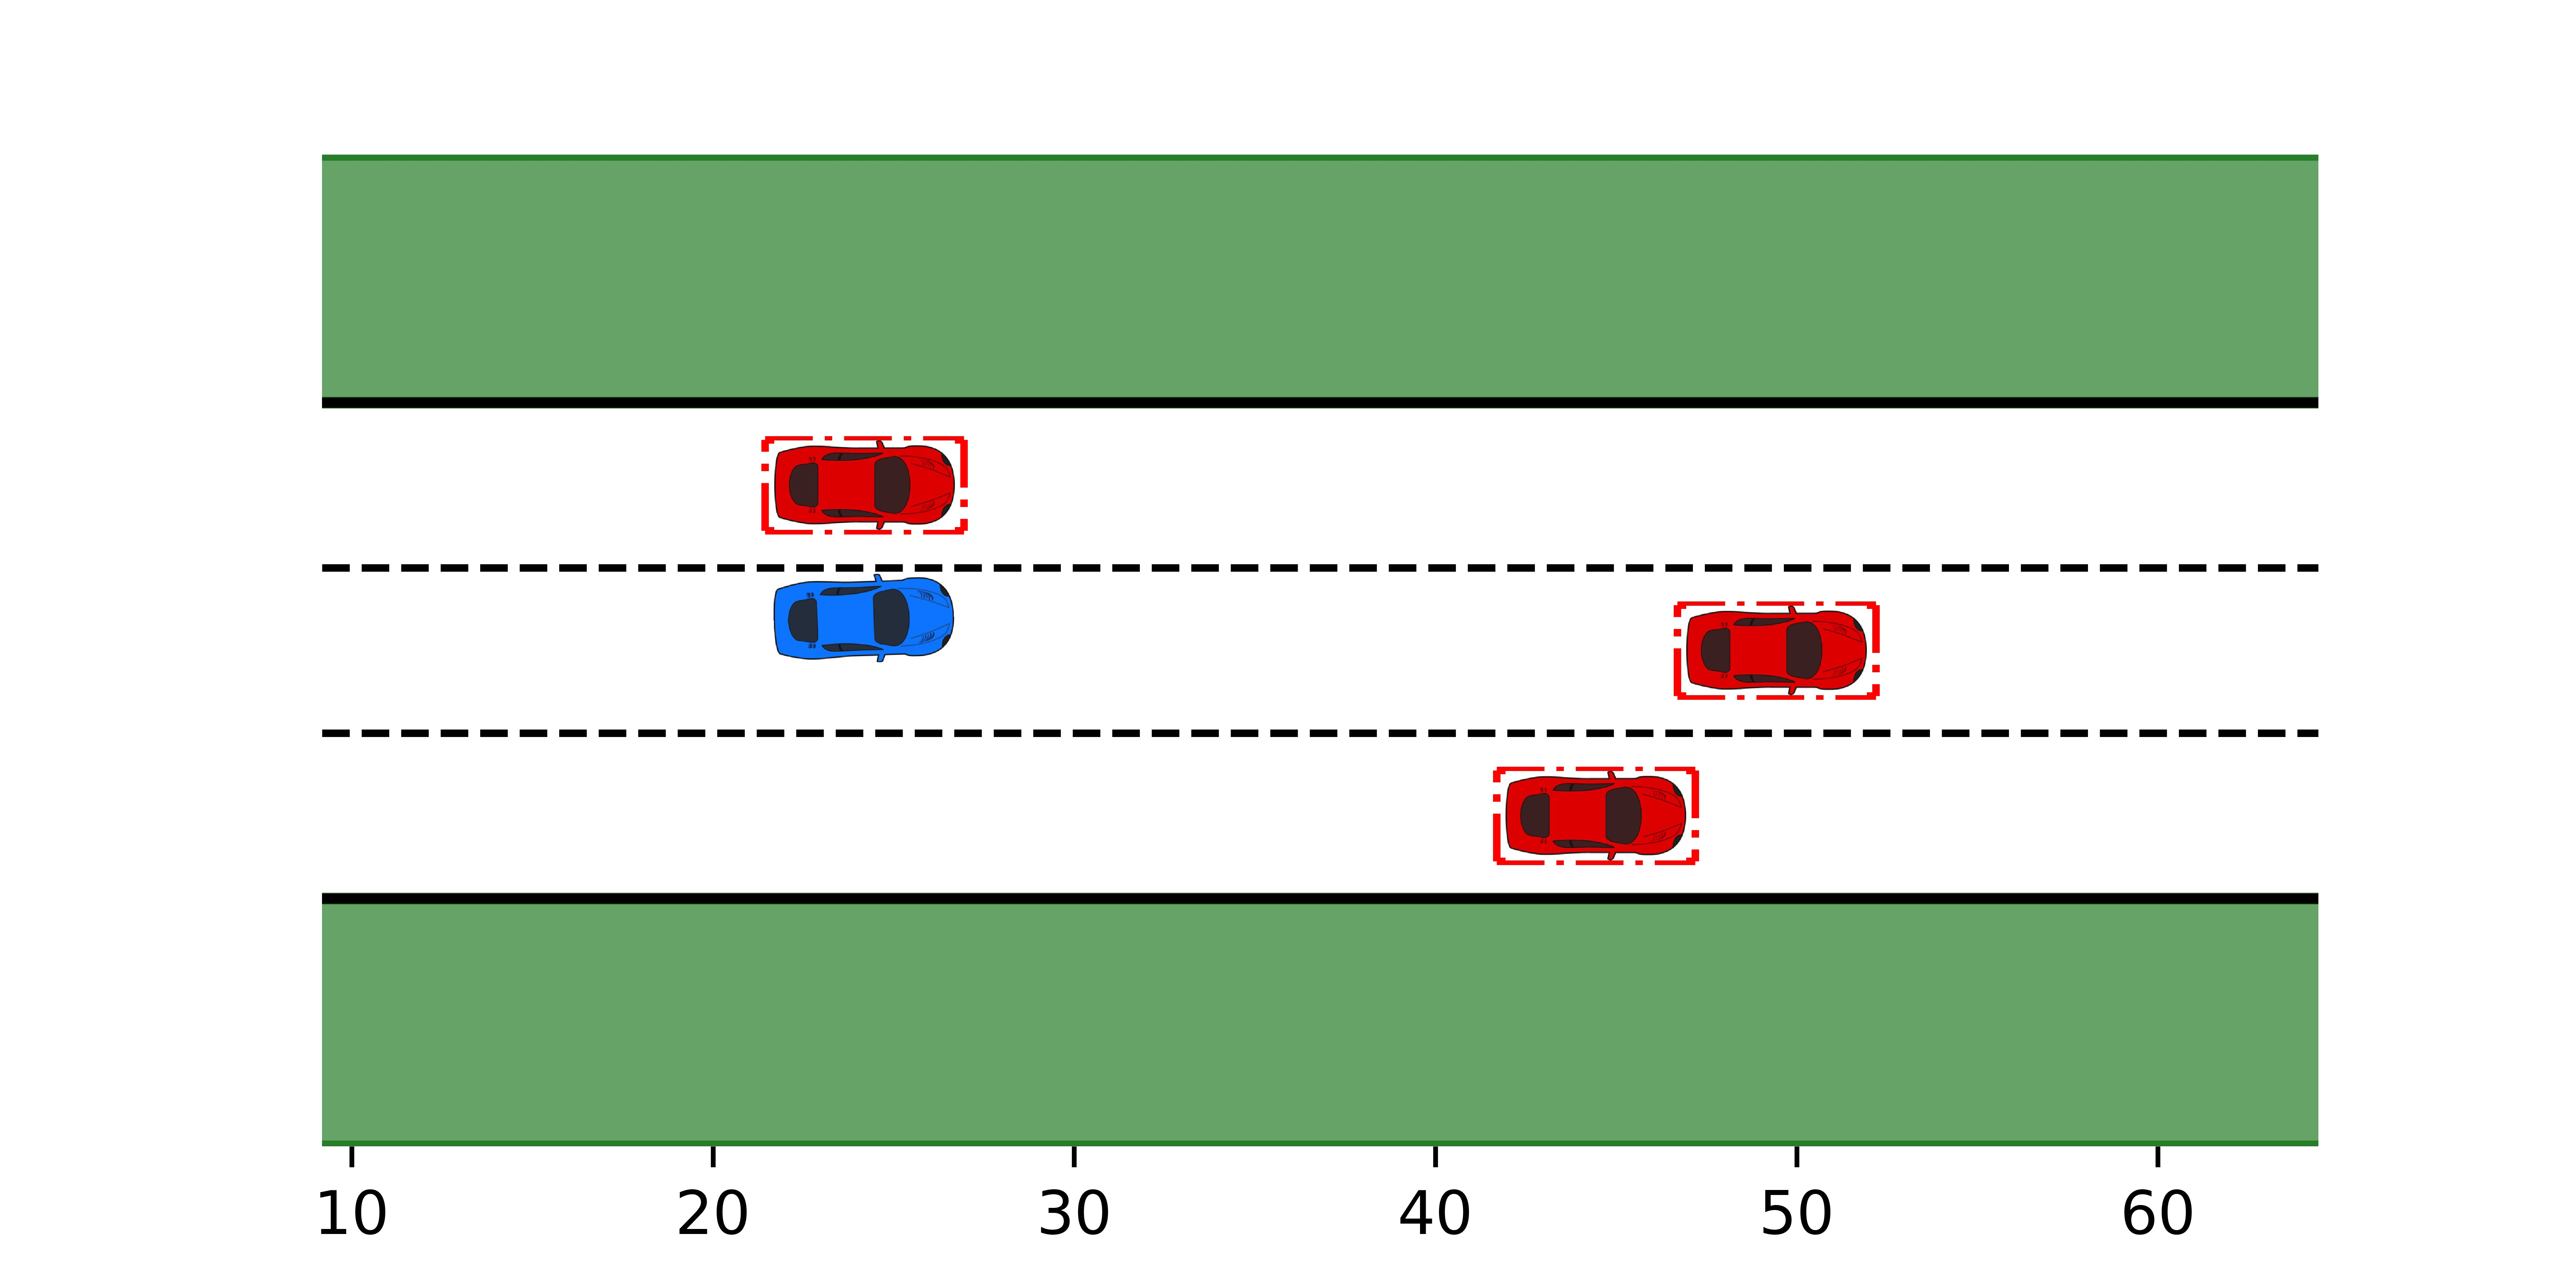
\includegraphics[clip, trim = {1.5cm 0.25cm 1.5cm 0.25cm}]{plot_agg2.jpg}};
			\node (con2)[ right = 1cm of adp2, minimum width = 0.cm, minimum height = 0cm, inner sep = 0pt]{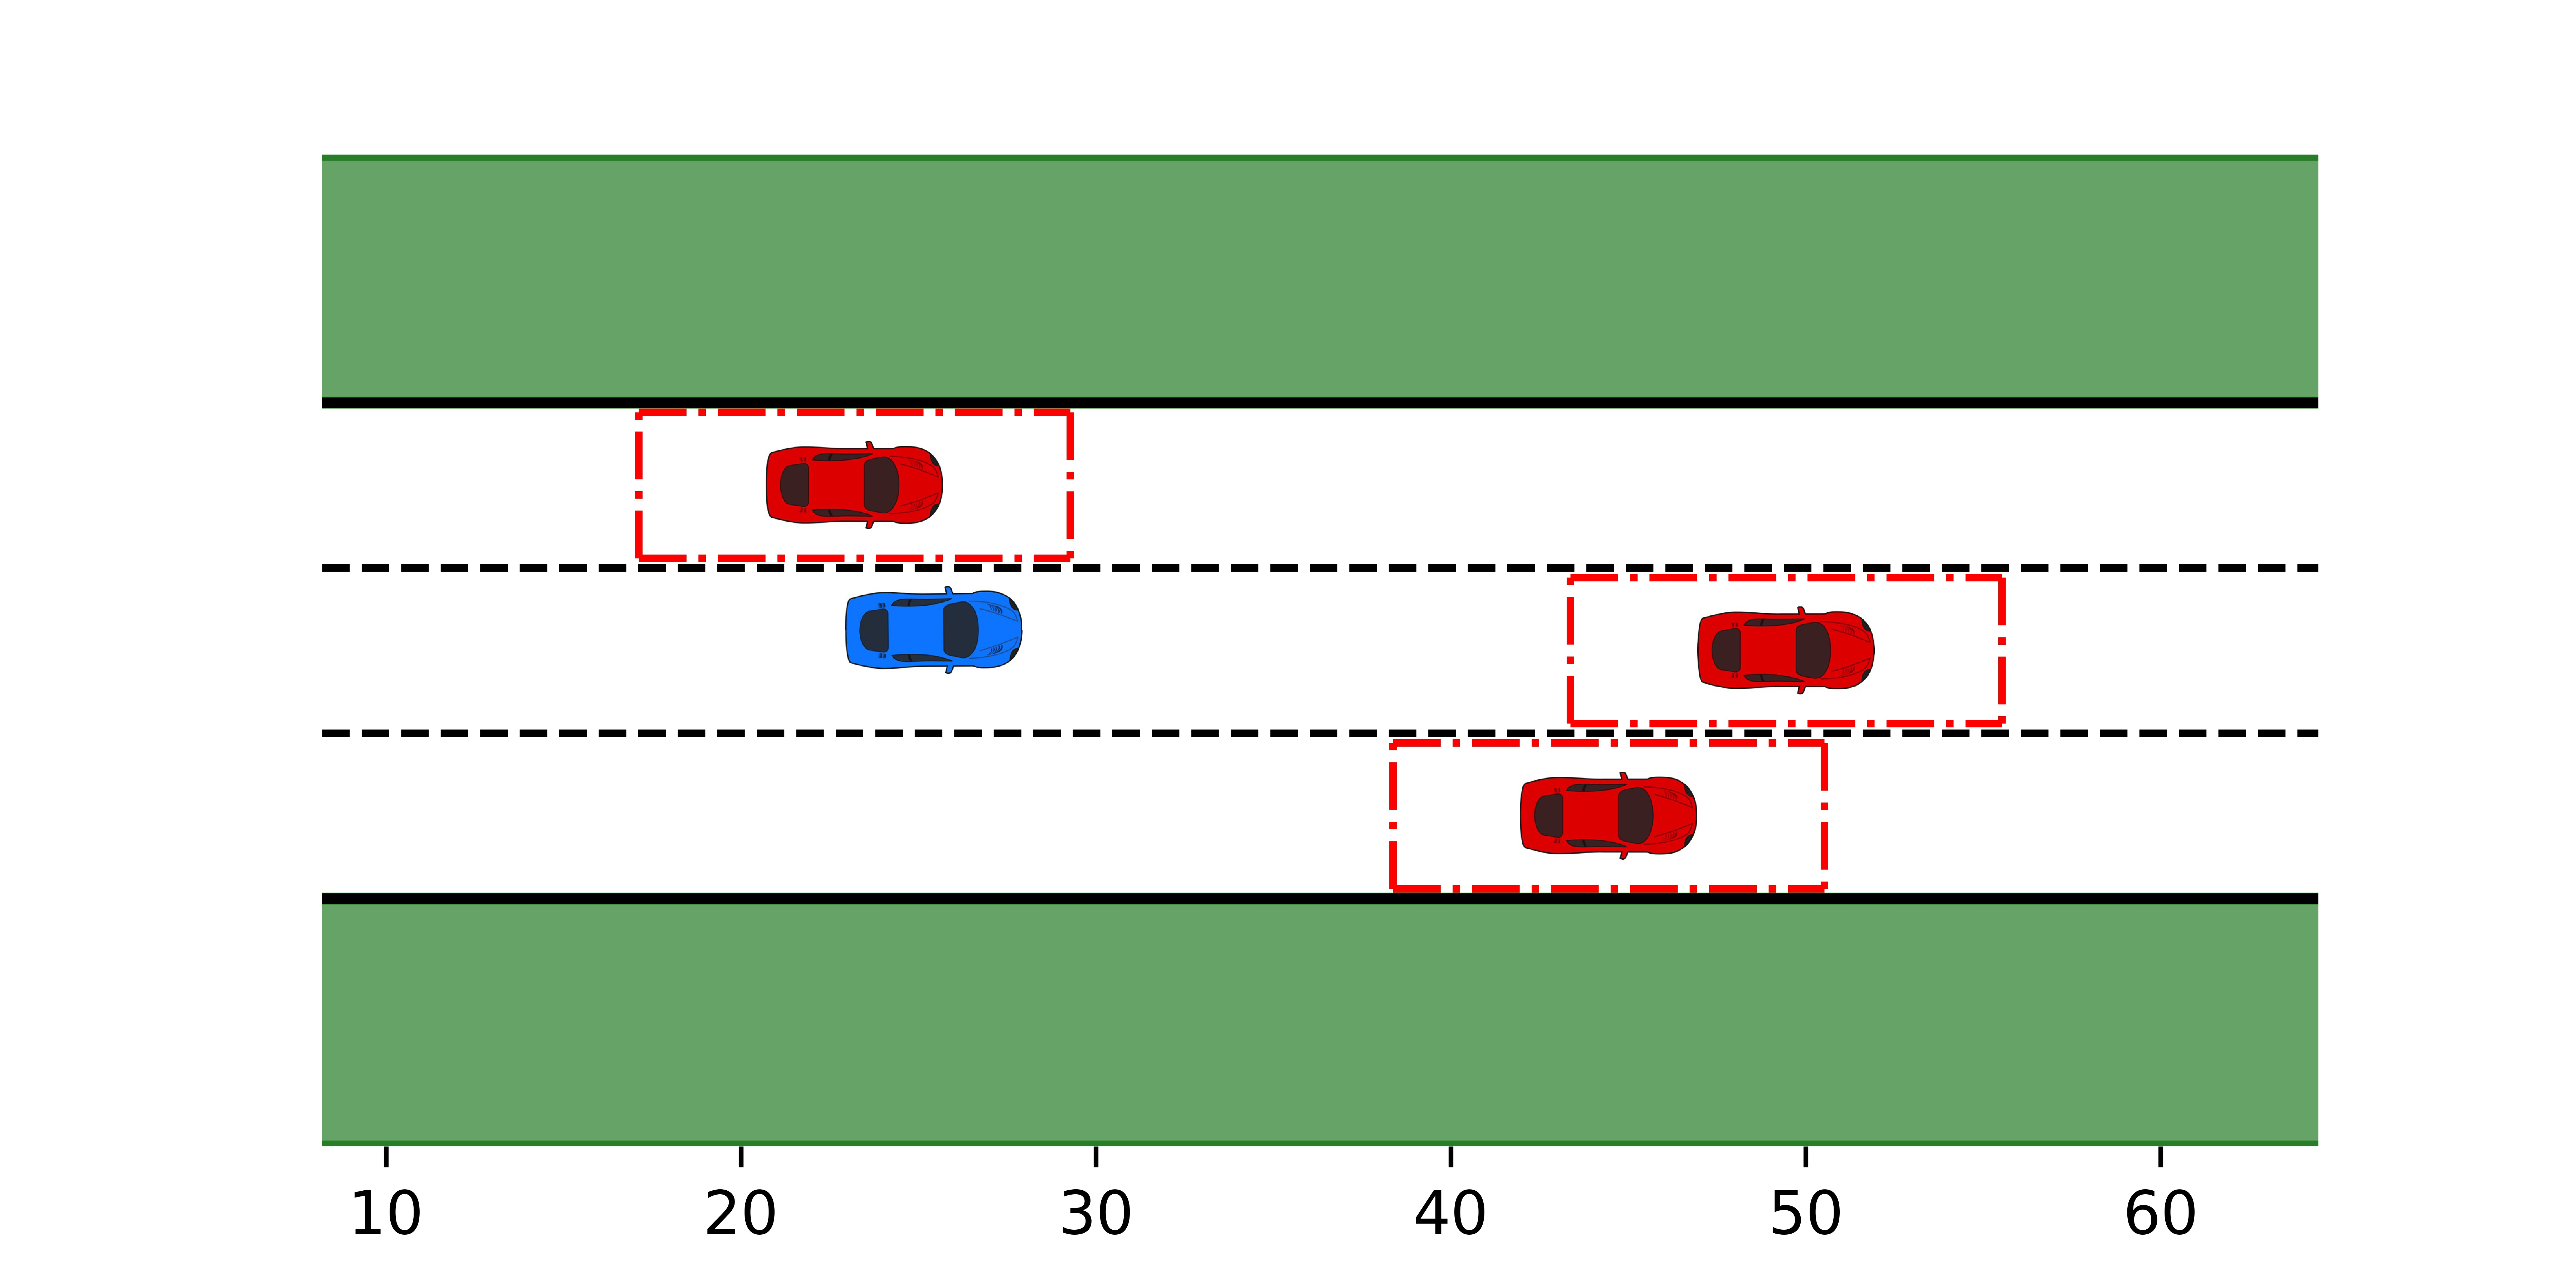
\includegraphics[clip, trim = {1.5cm 0.25cm 1.5cm 0.25cm}]{plot_con2.jpg}};
			
			
			\node (adp3)[below  = 1.cm of adp2, minimum width = 0.cm, minimum height = 0cm, inner sep = 0pt]{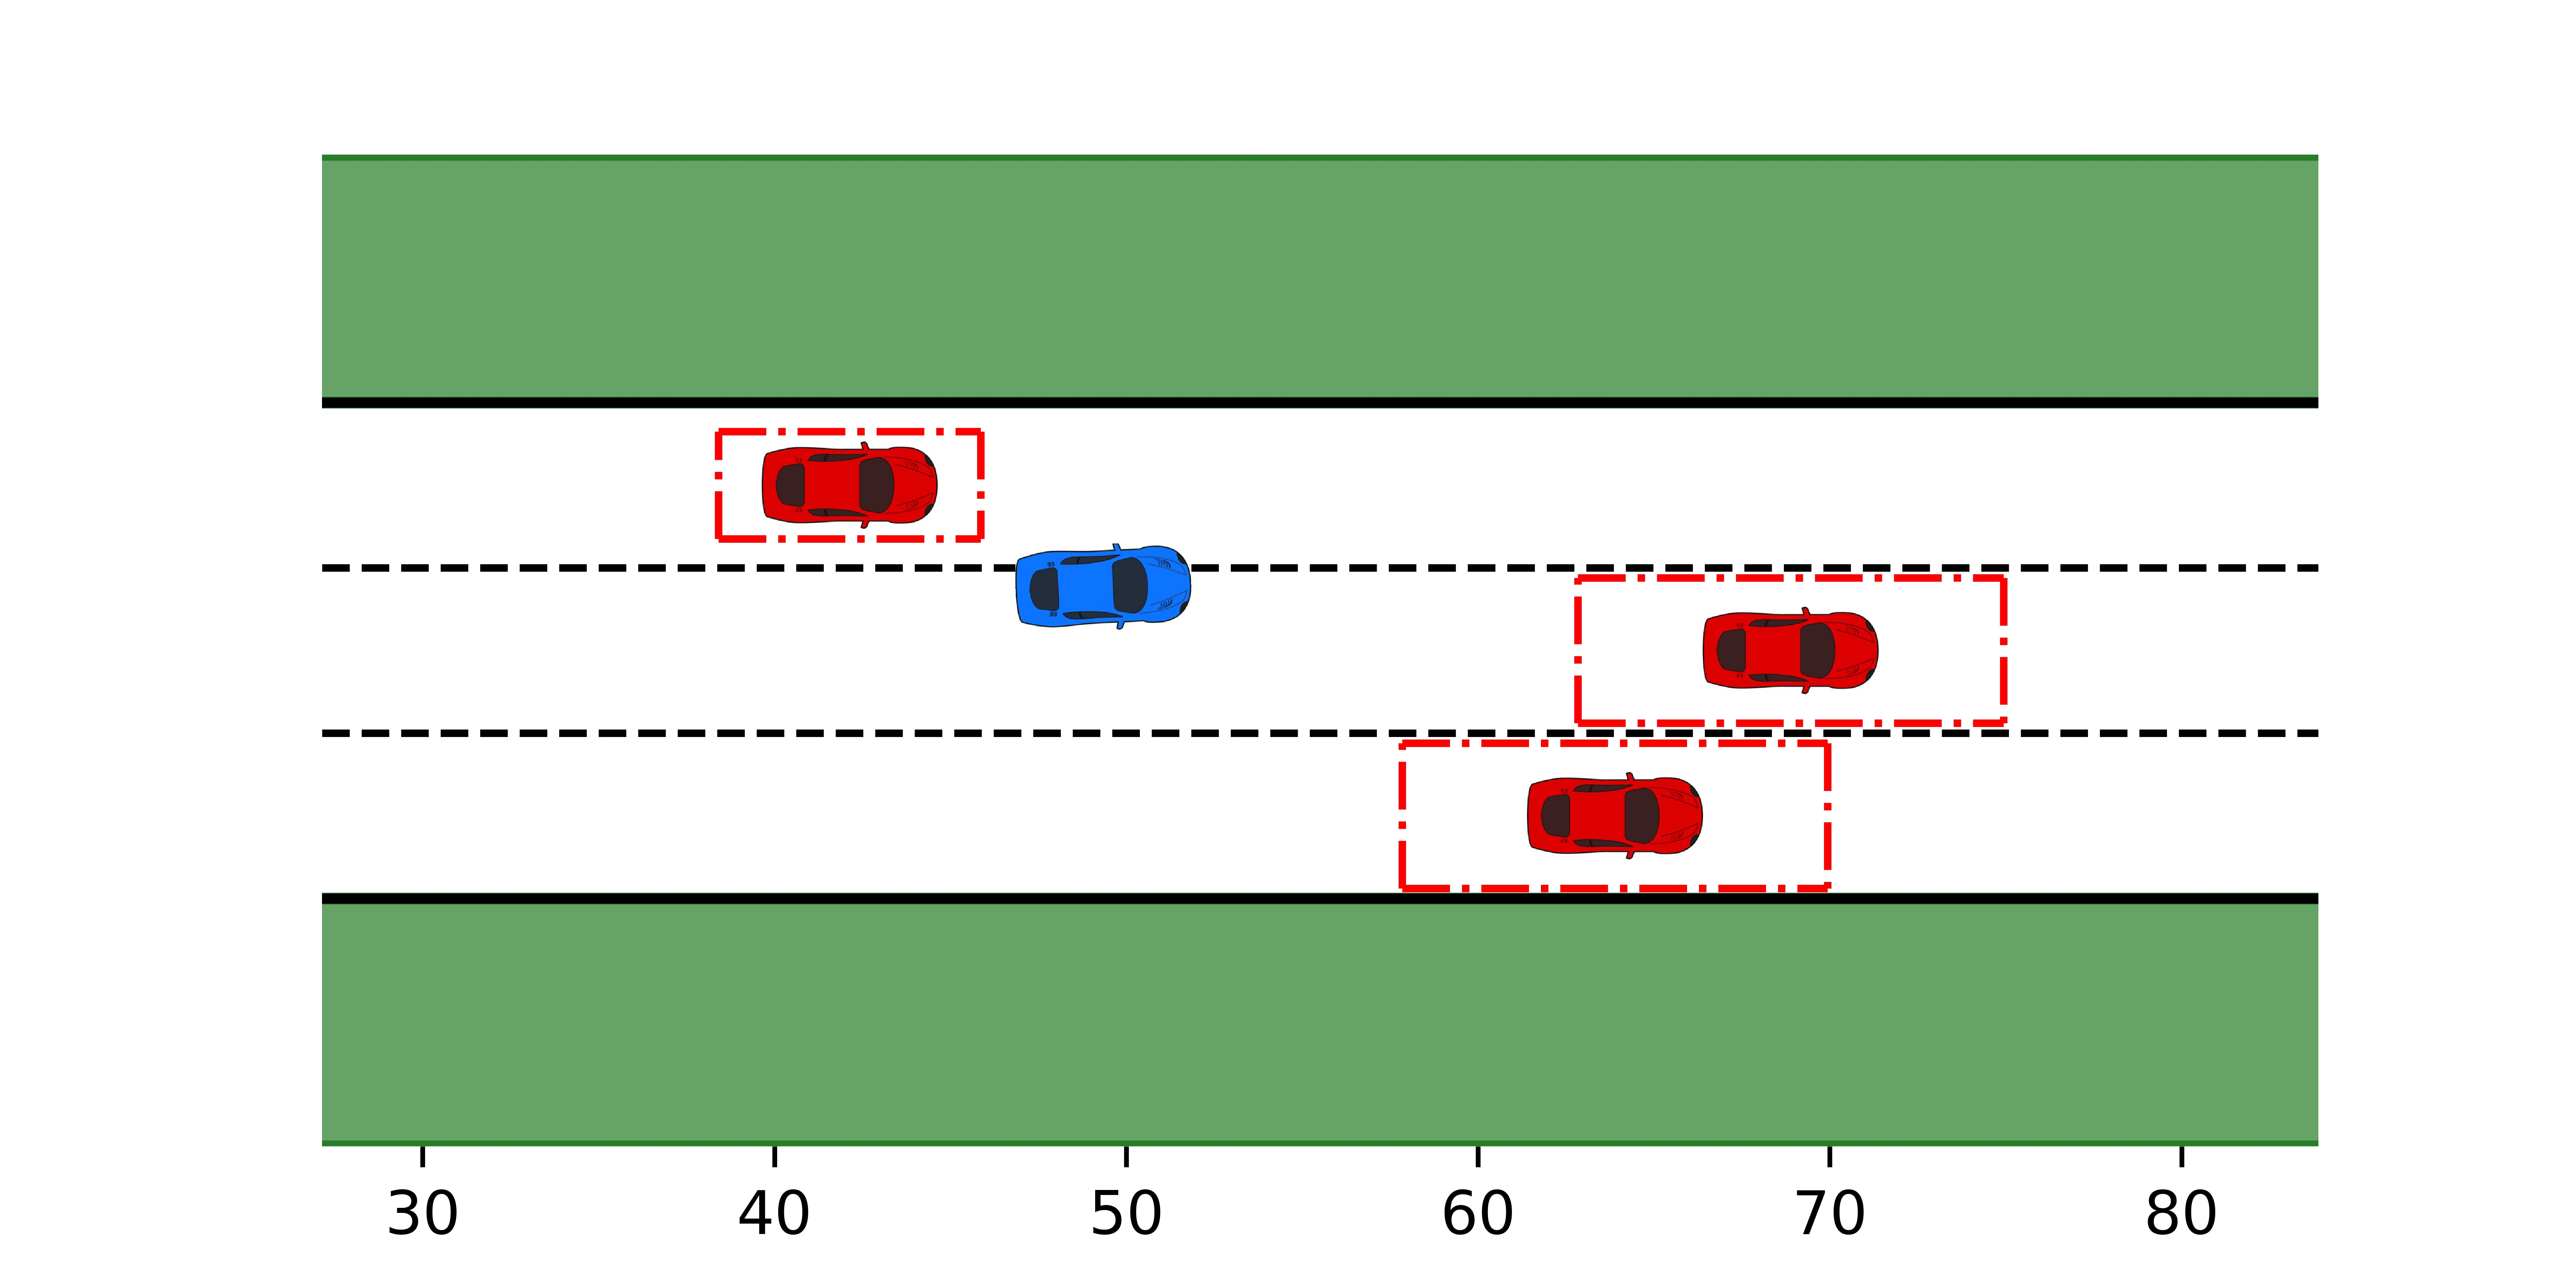
\includegraphics[clip, trim = {1.5cm 0.25cm 1.5cm 0.25cm}]{plot_adp4.jpg}};
			\node (agg3)[left = 1cm of adp3, minimum width = 0.cm, minimum height = 0cm, inner sep = 0pt]{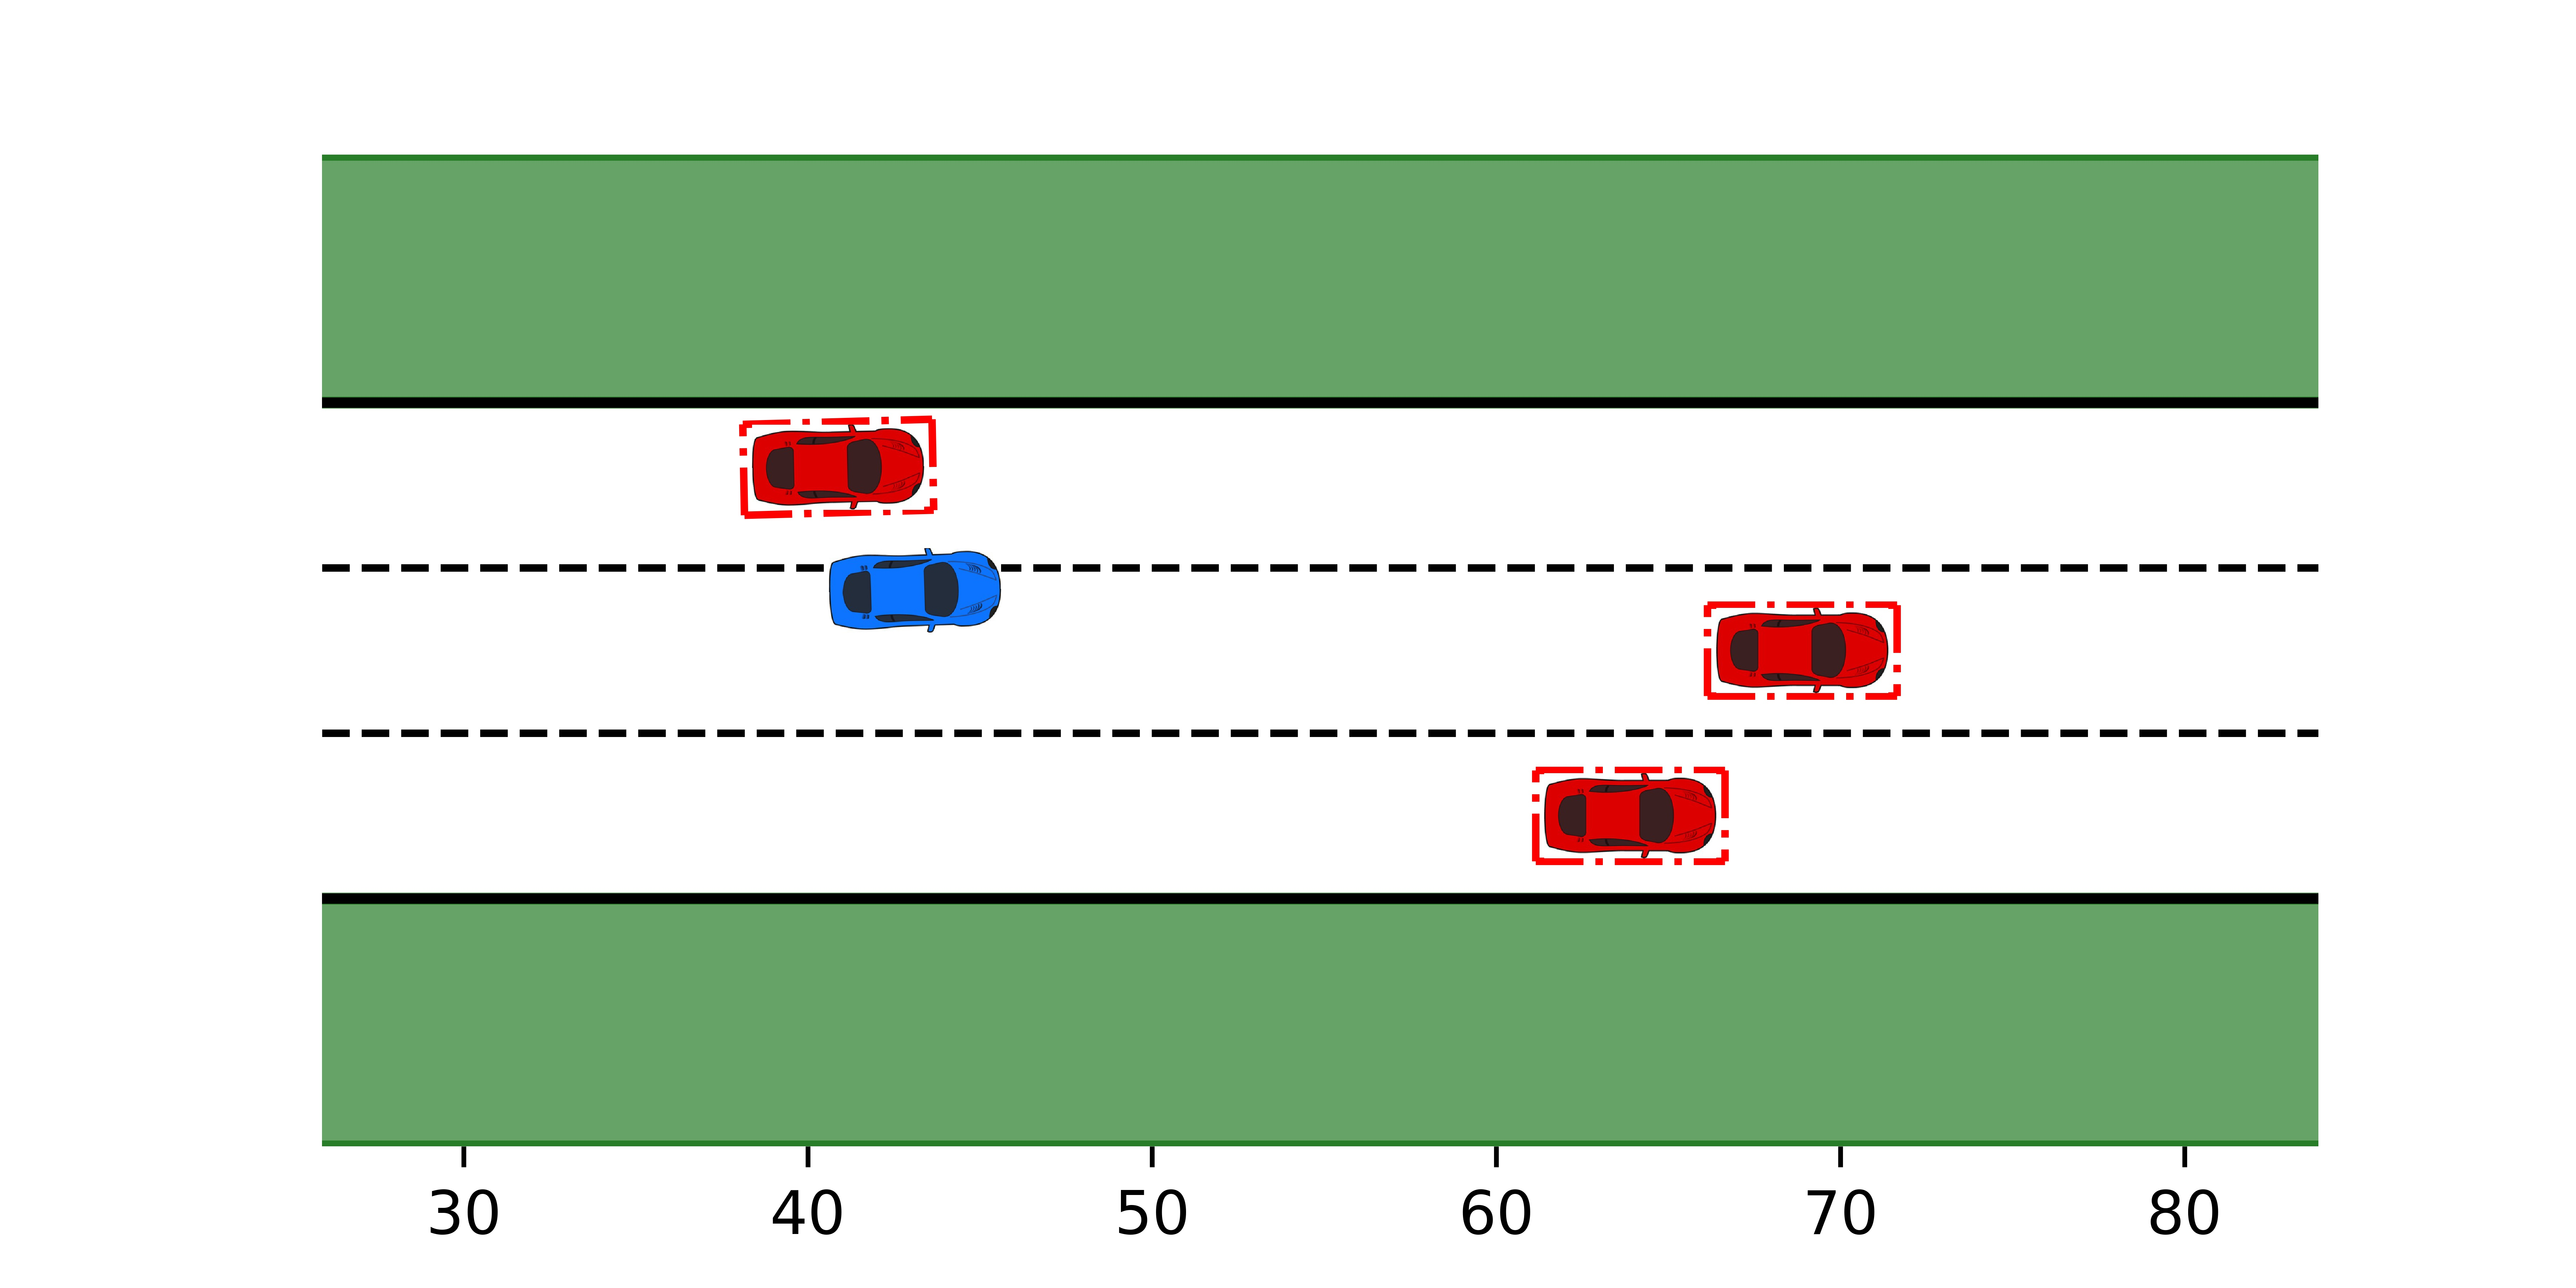
\includegraphics[clip, trim = {1.5cm 0.25cm 1.5cm 0.25cm}]{plot_agg4.jpg}};
			\node (con3)[ right = 1cm of adp3, minimum width = 0.cm, minimum height = 0cm, inner sep = 0pt]{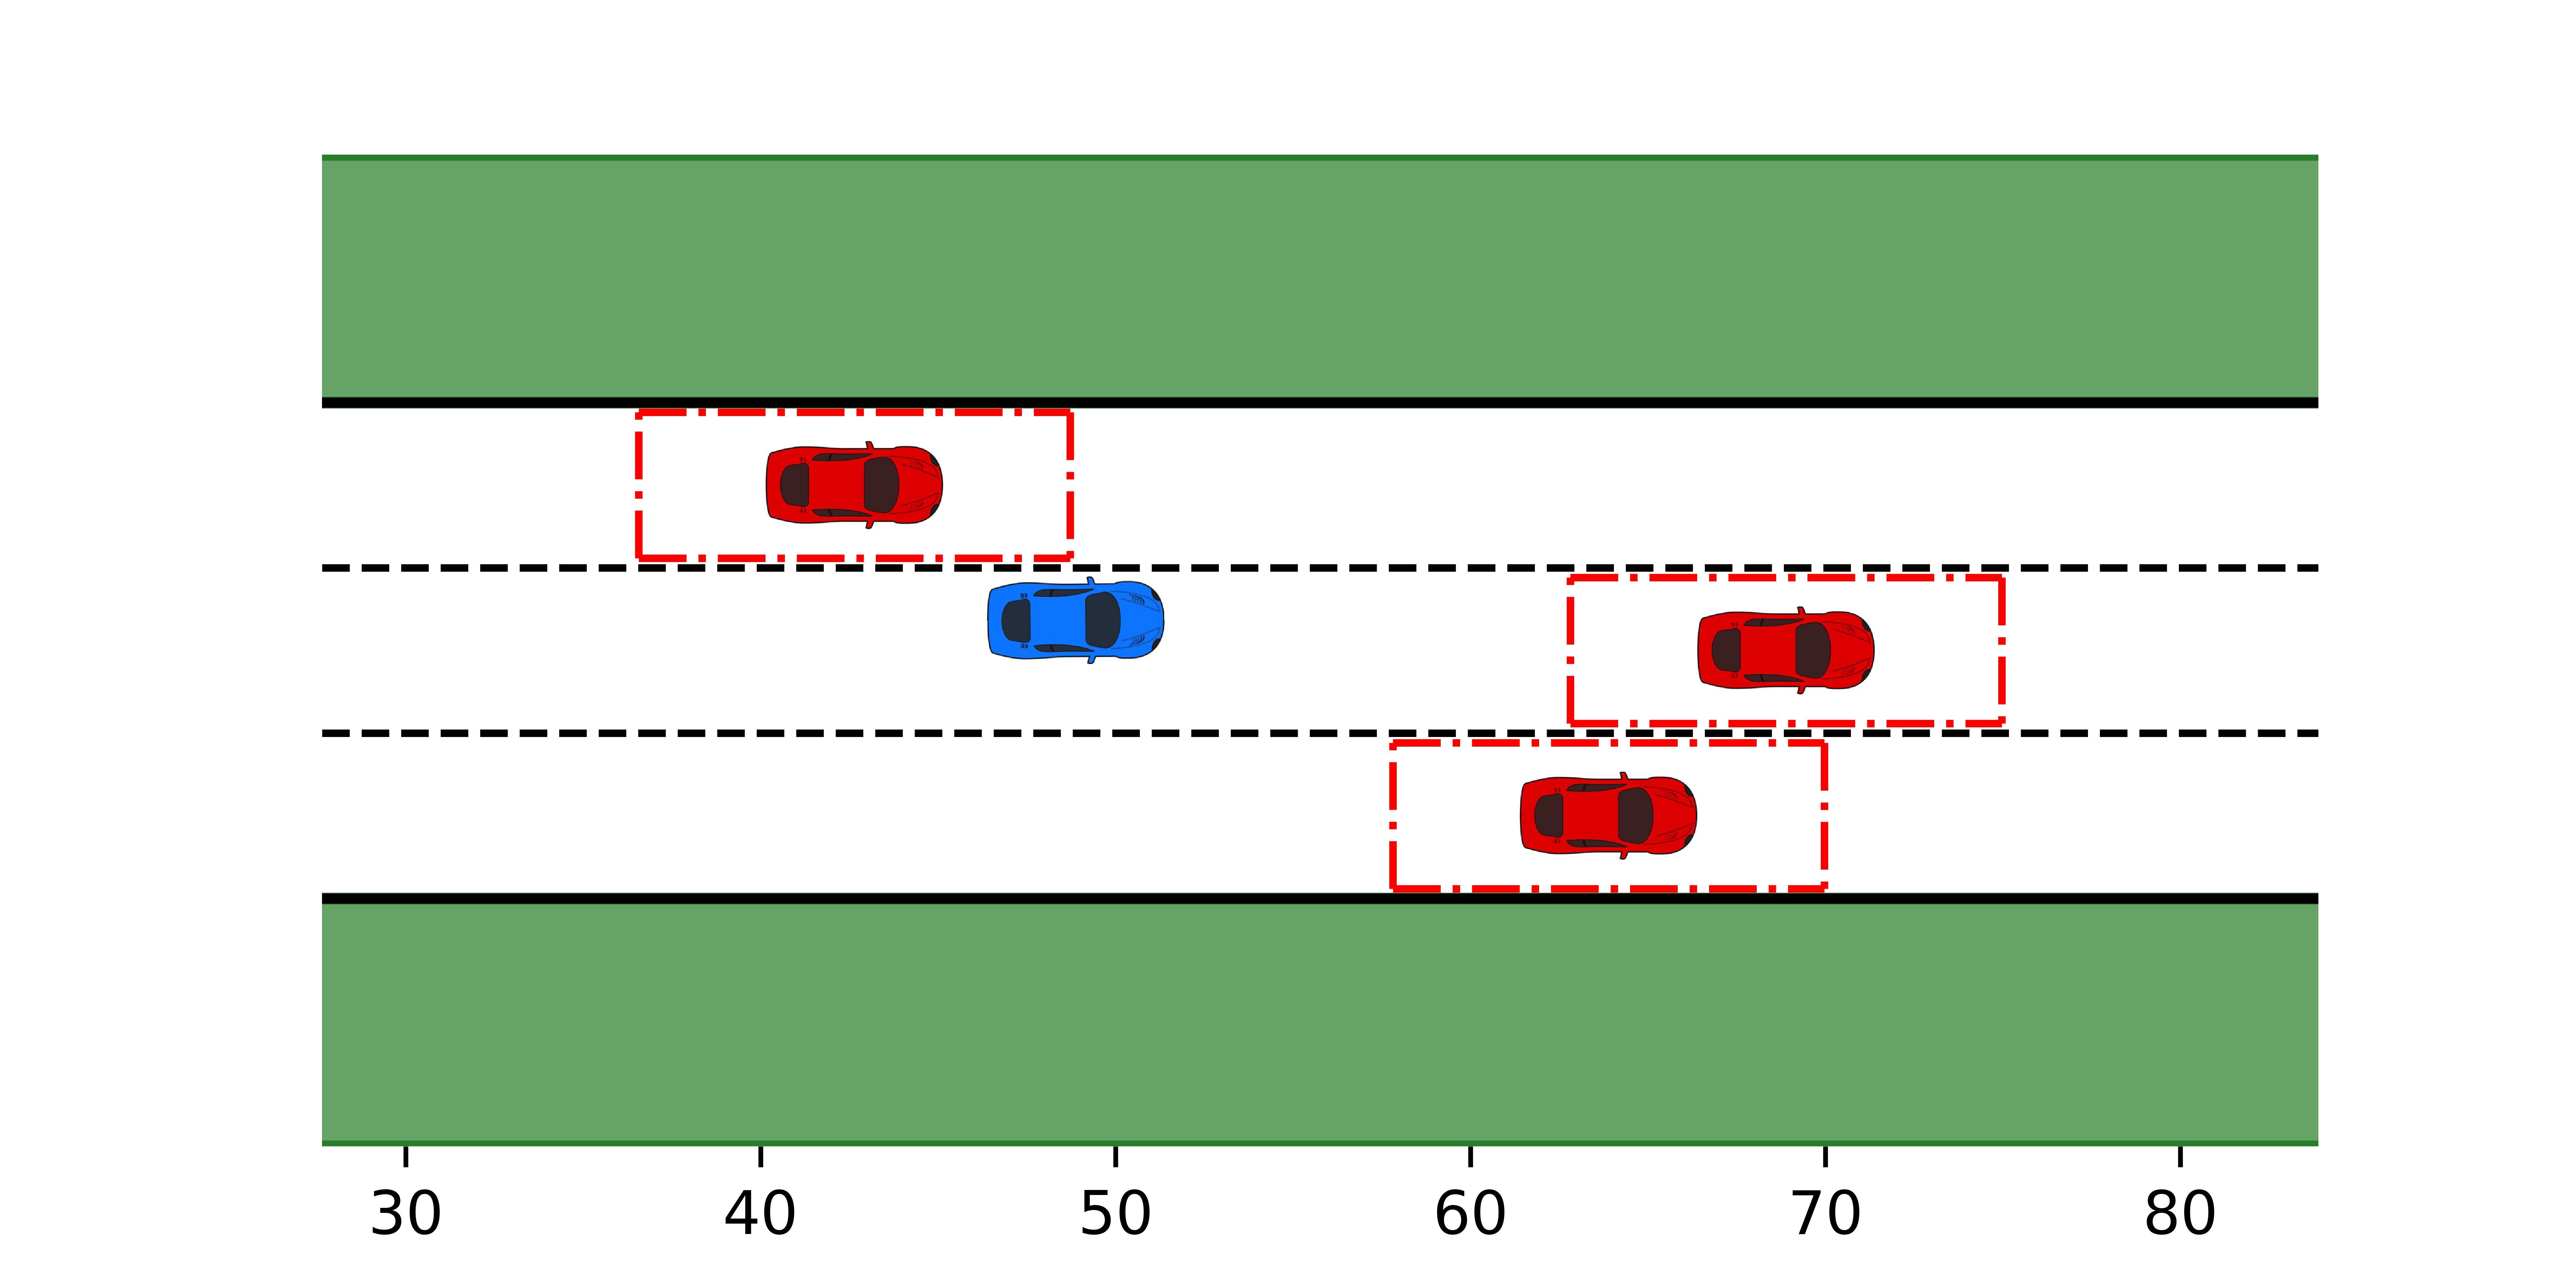
\includegraphics[clip, trim = {1.5cm 0.25cm 1.5cm 0.25cm}]{plot_con4.jpg}};
			
			
			\node (adp4)[below  = 1.cm of adp3, minimum width = 0.cm, minimum height = 0cm, inner sep = 0pt]{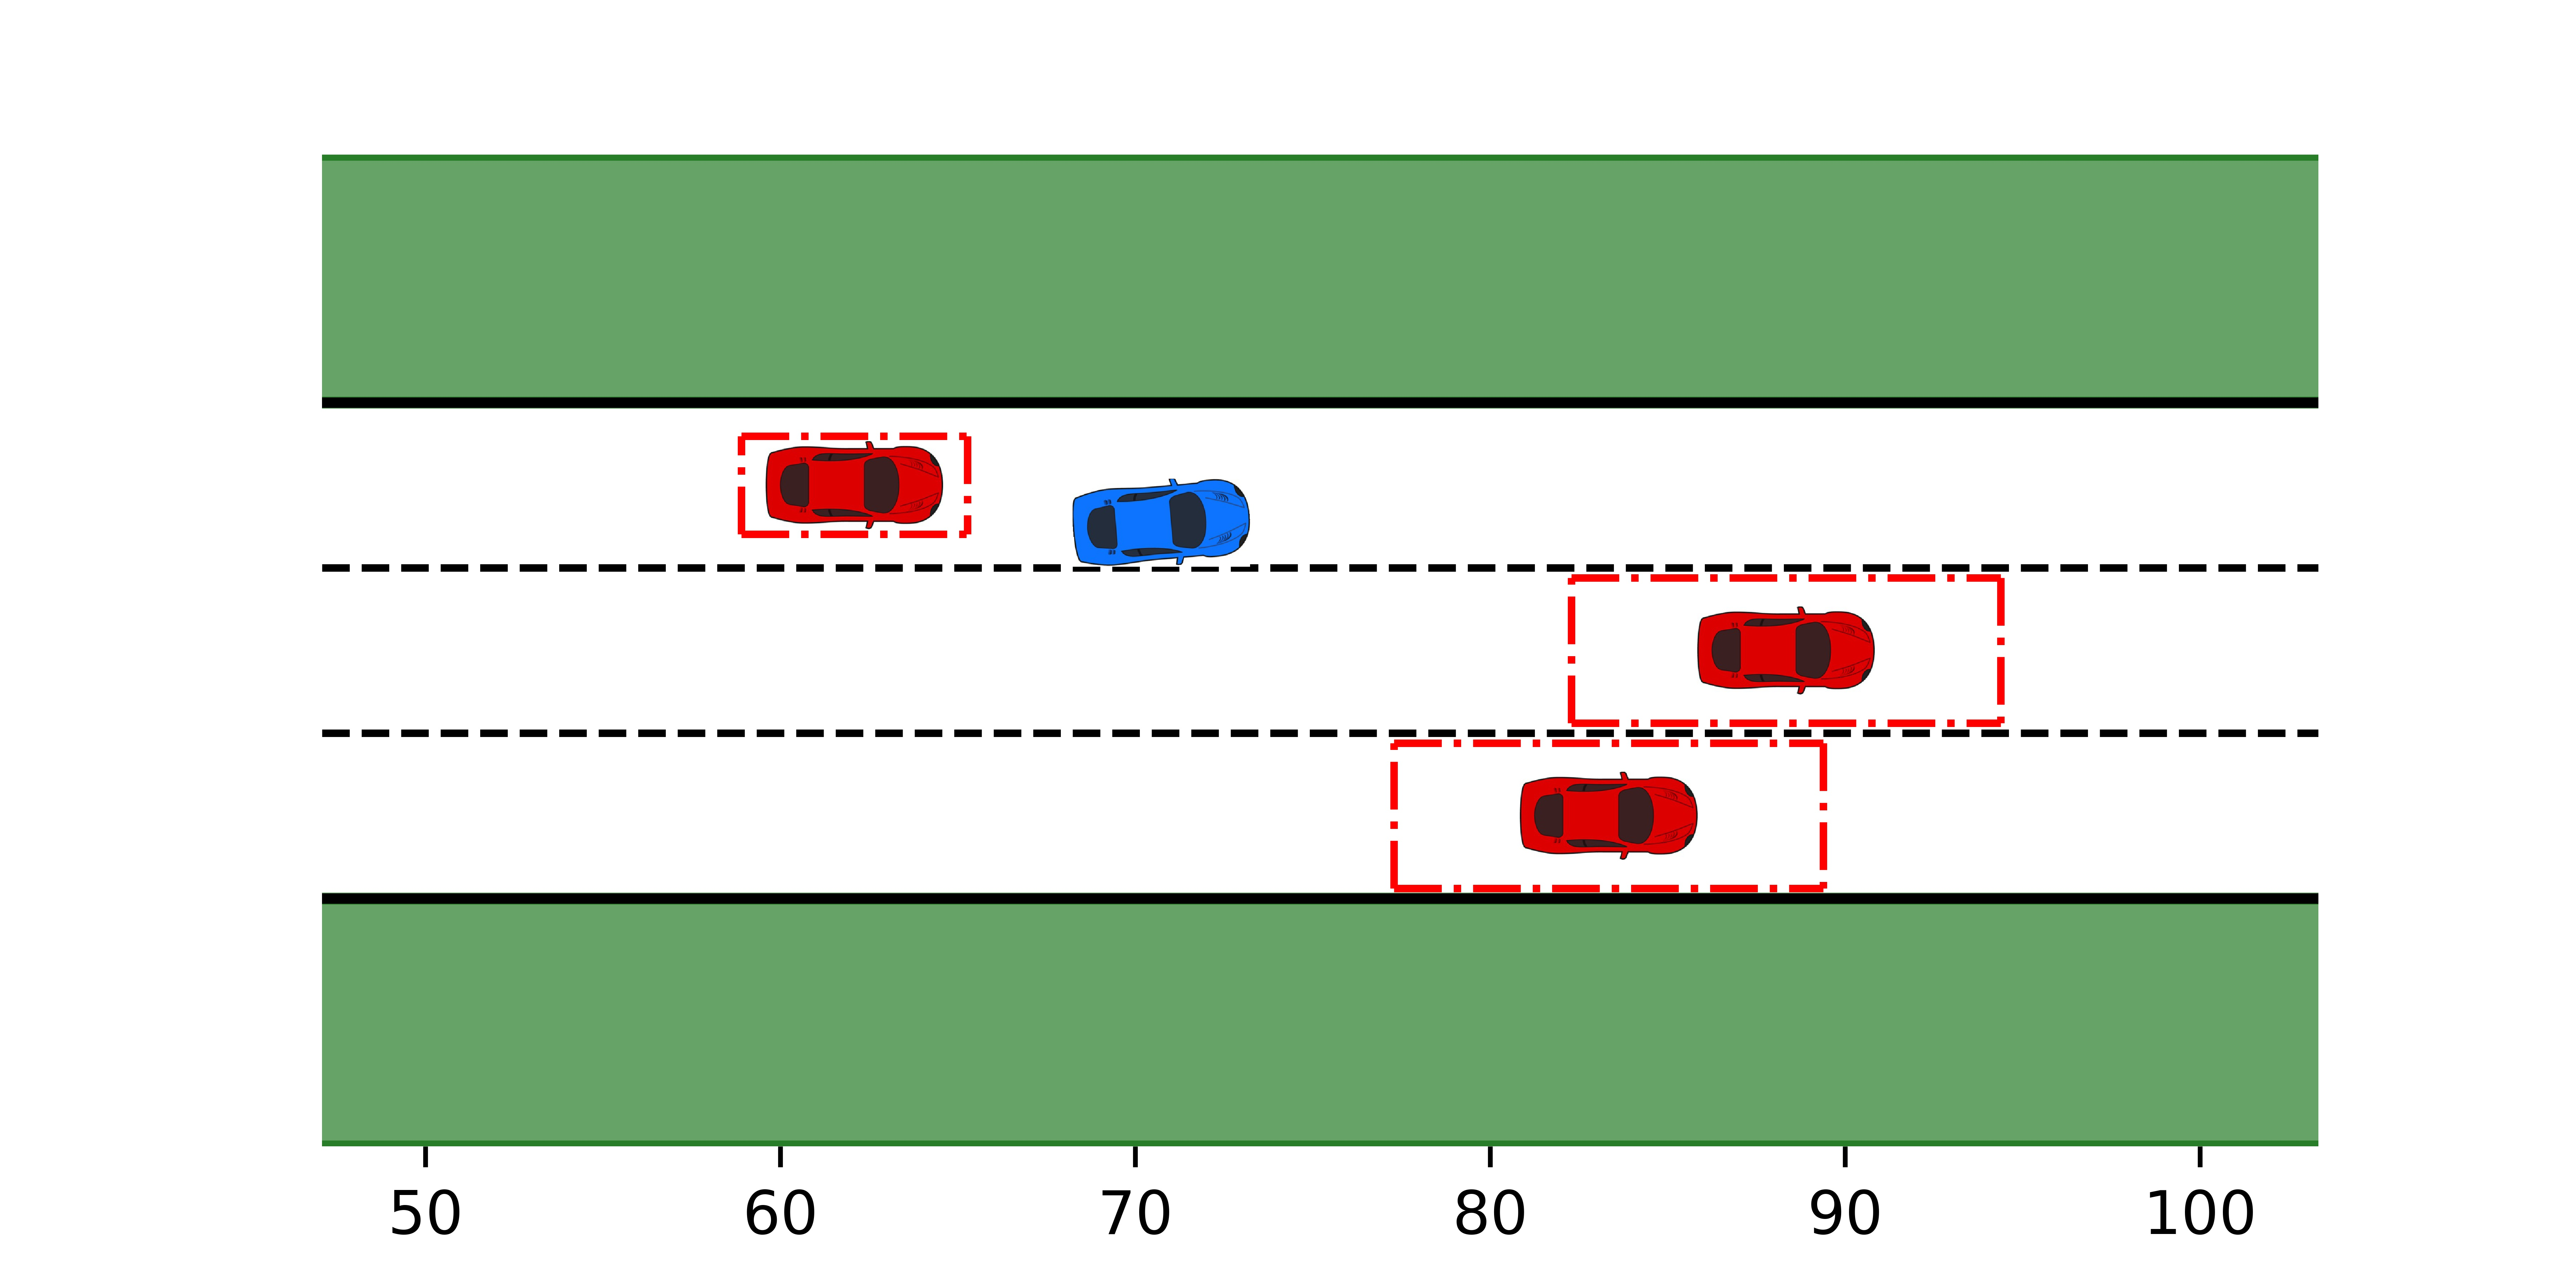
\includegraphics[clip, trim = {1.5cm 0.25cm 1.5cm 0.25cm}]{plot_adp6.jpg}};
			\node (agg4)[left = 1cm of adp4, minimum width = 0.cm, minimum height = 0cm, inner sep = 0pt]{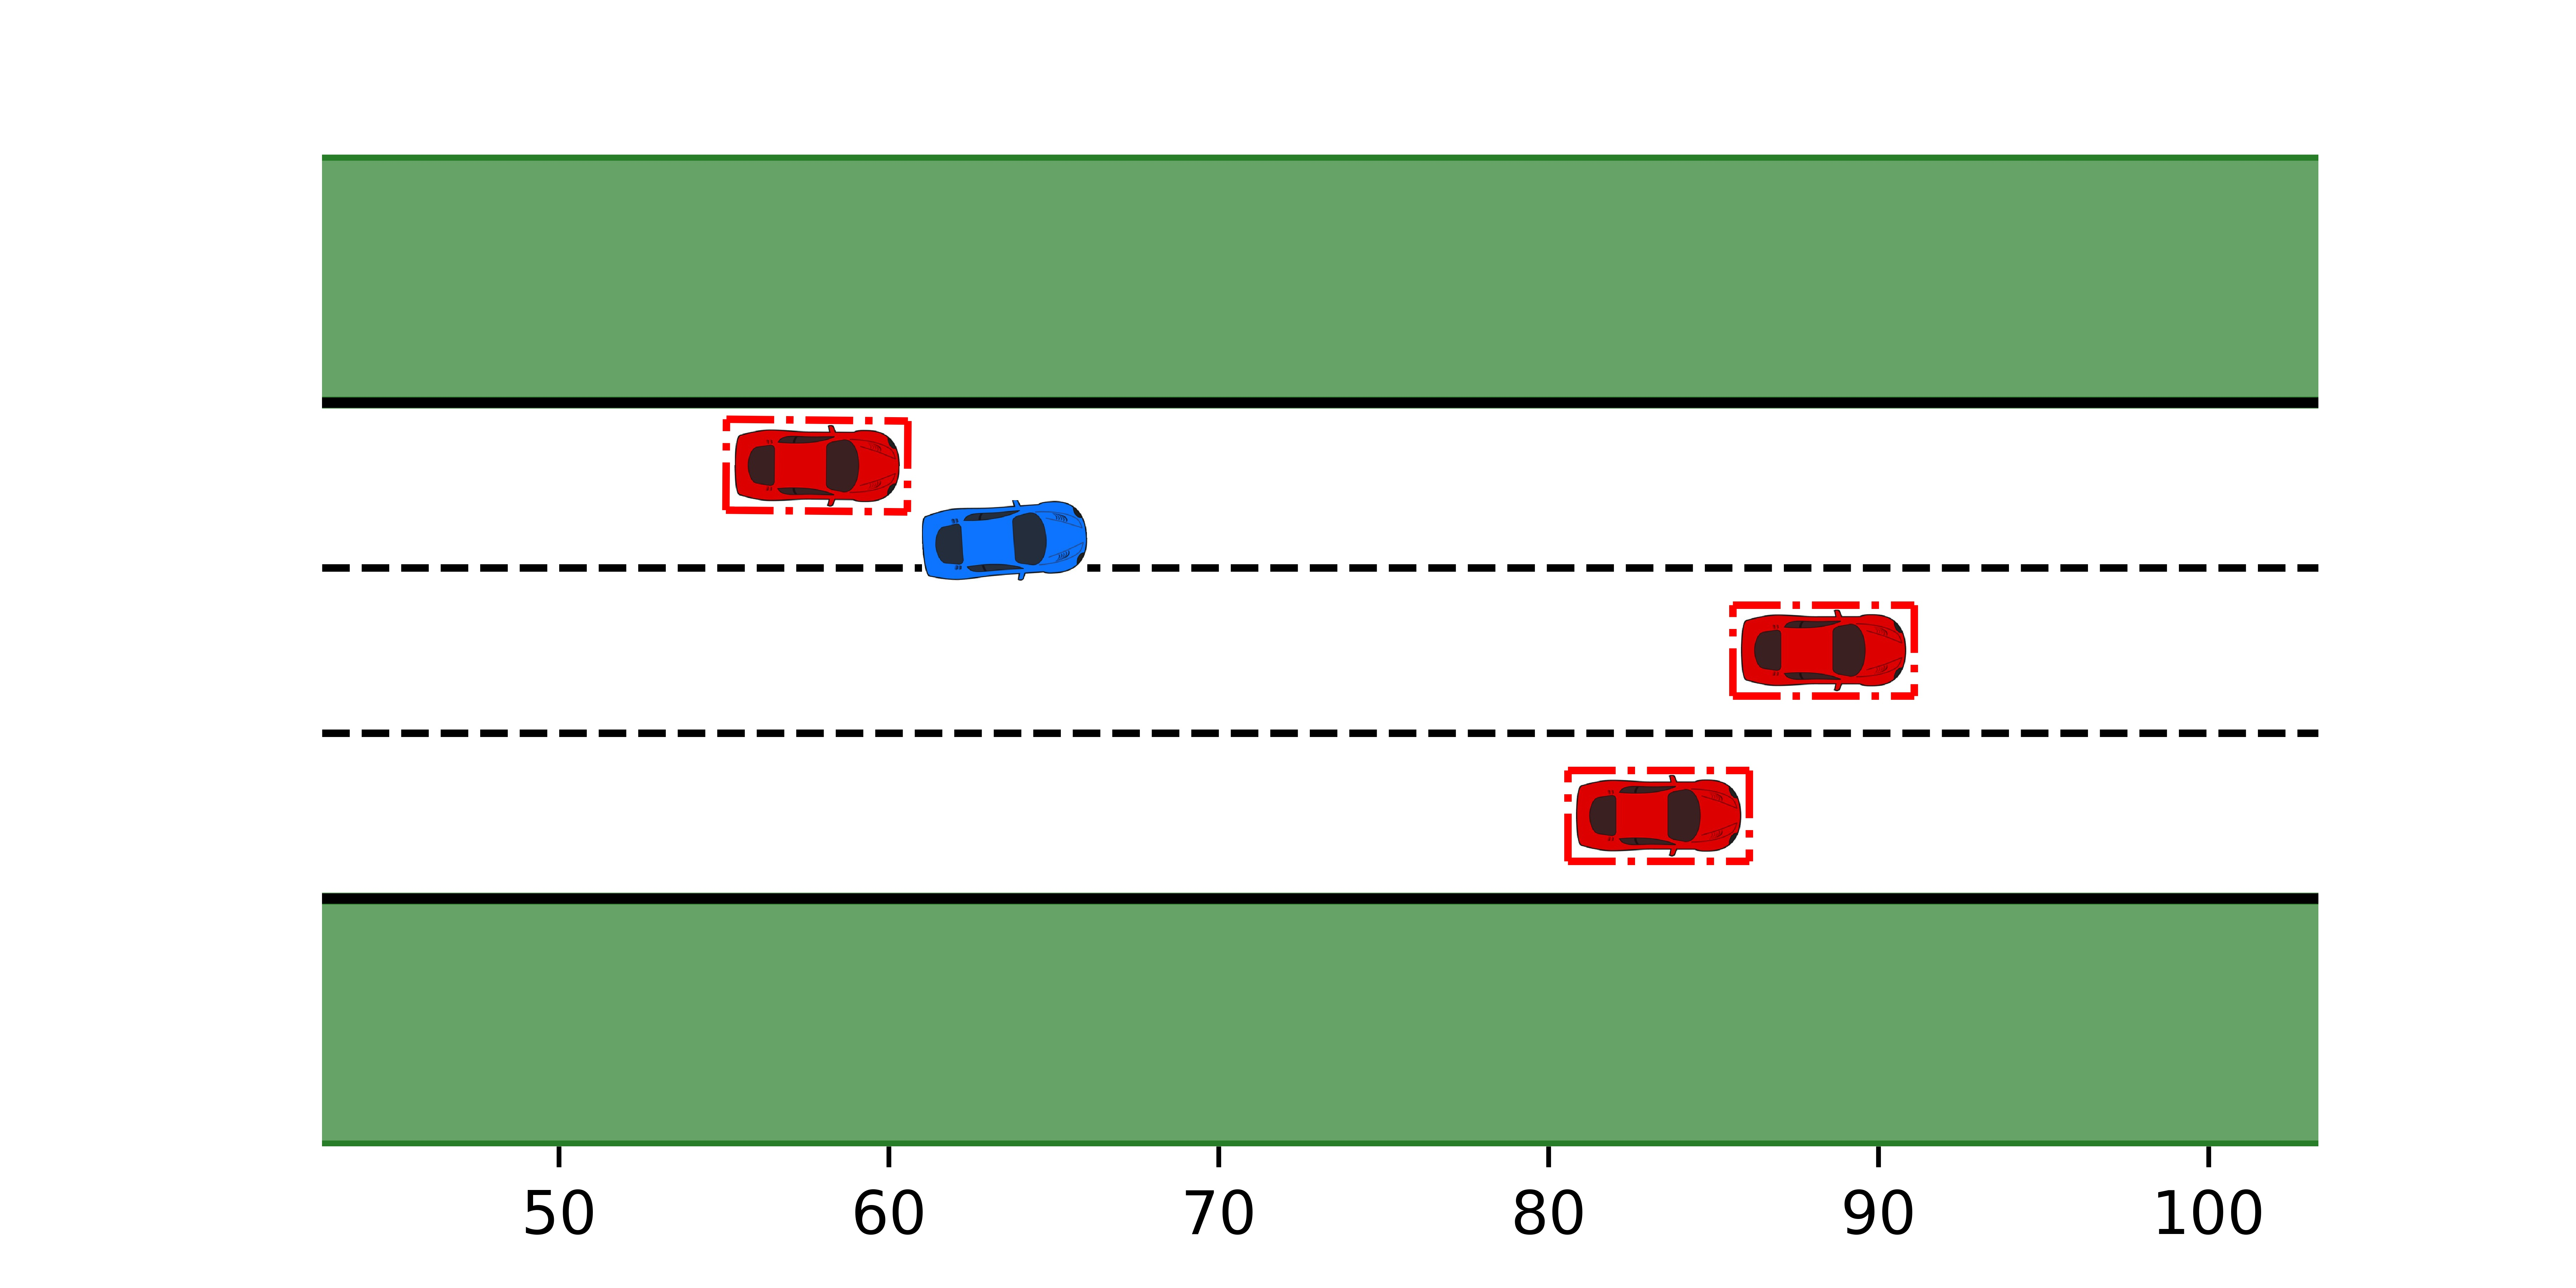
\includegraphics[clip, trim = {1.5cm 0.25cm 1.5cm 0.25cm}]{plot_agg6.jpg}};
			\node (con4)[ right = 1cm of adp4, minimum width = 0.cm, minimum height = 0cm, inner sep = 0pt]{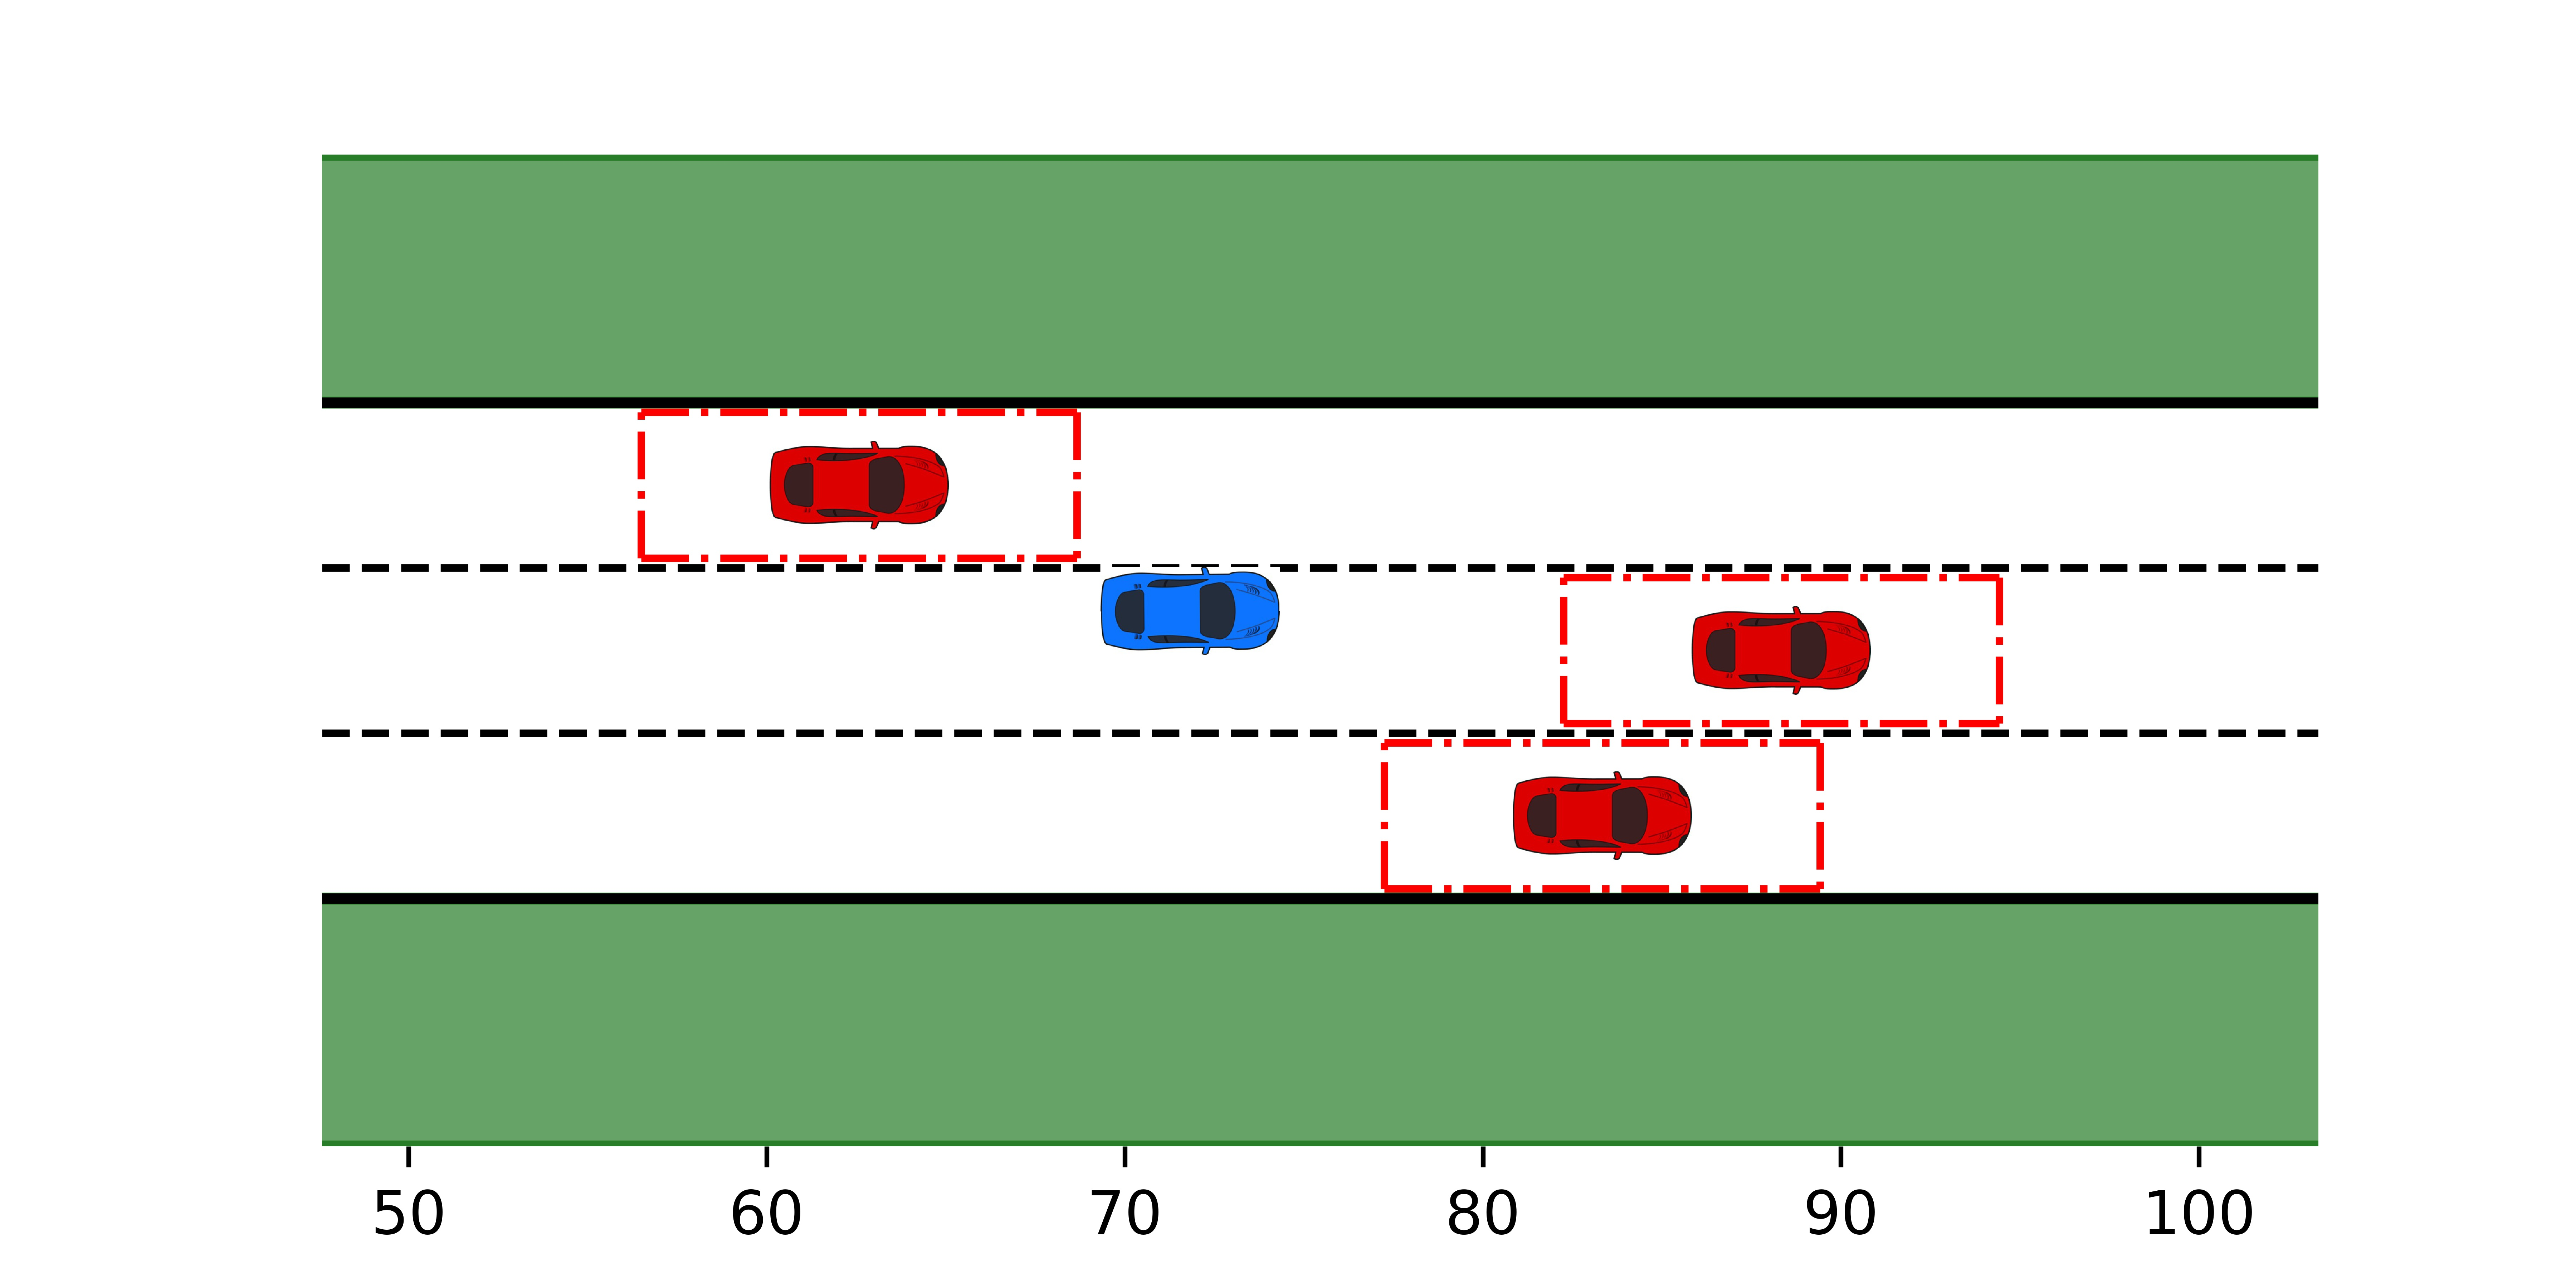
\includegraphics[clip, trim = {1.5cm 0.25cm 1.5cm 0.25cm}]{plot_con6.jpg}};
			
			\node (adp5)[below  = 1.cm of adp4, minimum width = 0.cm, minimum height = 0cm, inner sep = 0pt]{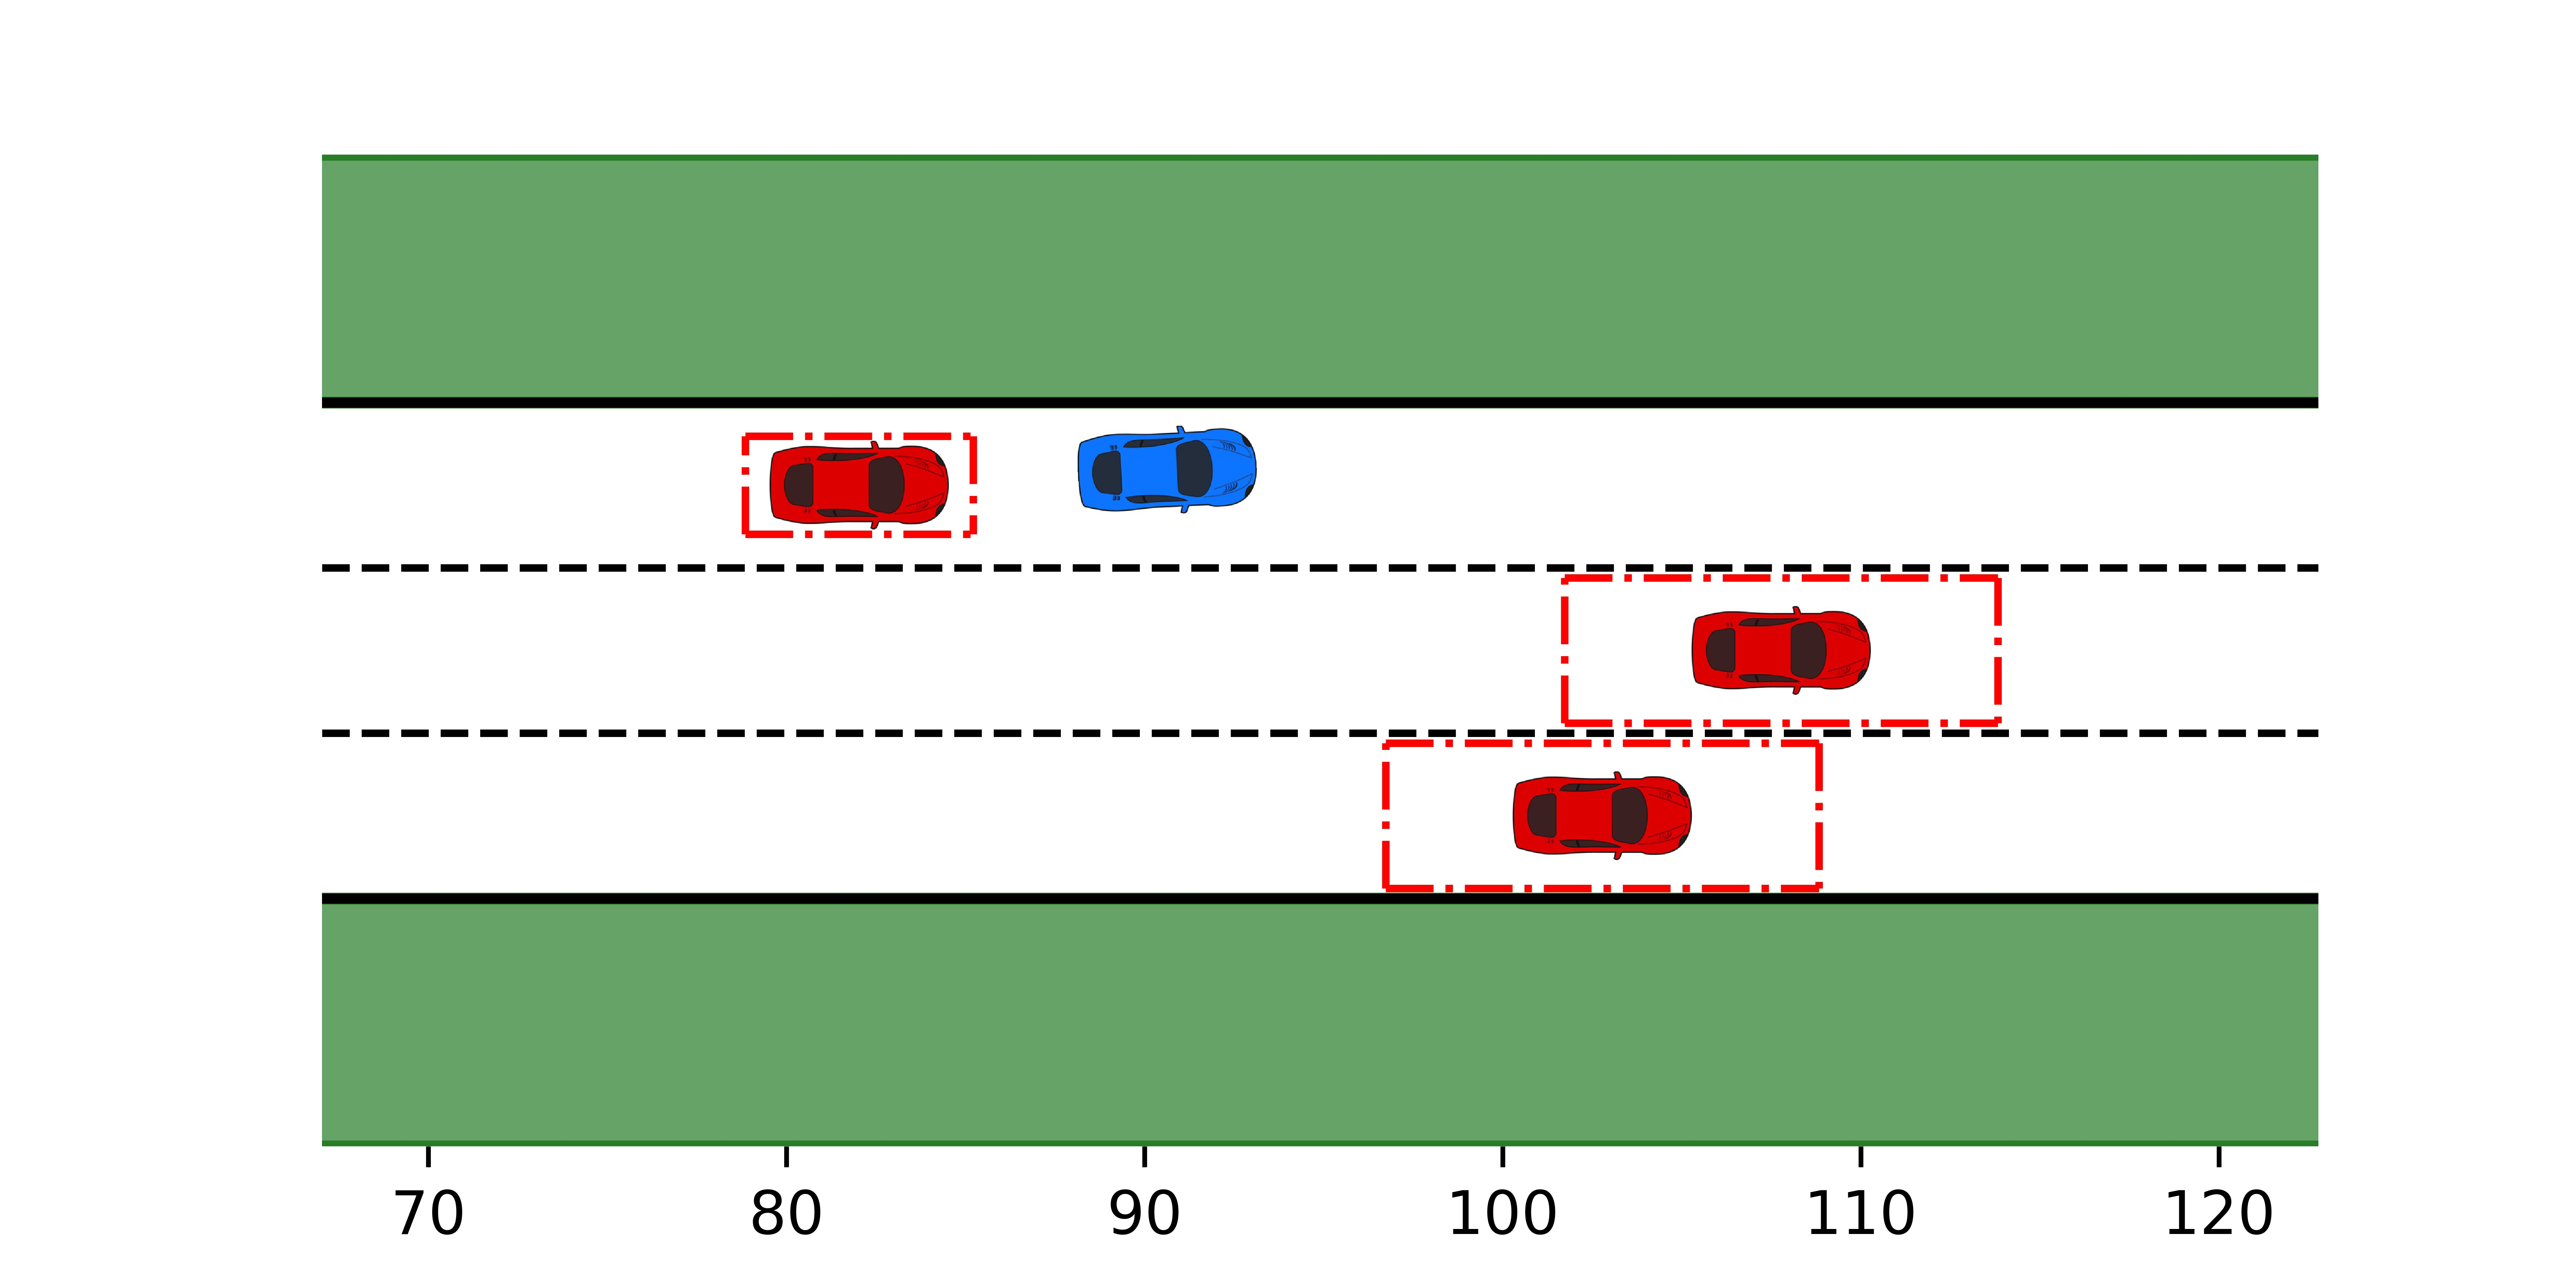
\includegraphics[clip, trim = {1.5cm 0.25cm 1.5cm 0.25cm}]{plot_adp8.jpg}};
			\node (agg5)[left = 1cm of adp5, minimum width = 0.cm, minimum height = 0cm, inner sep = 0pt]{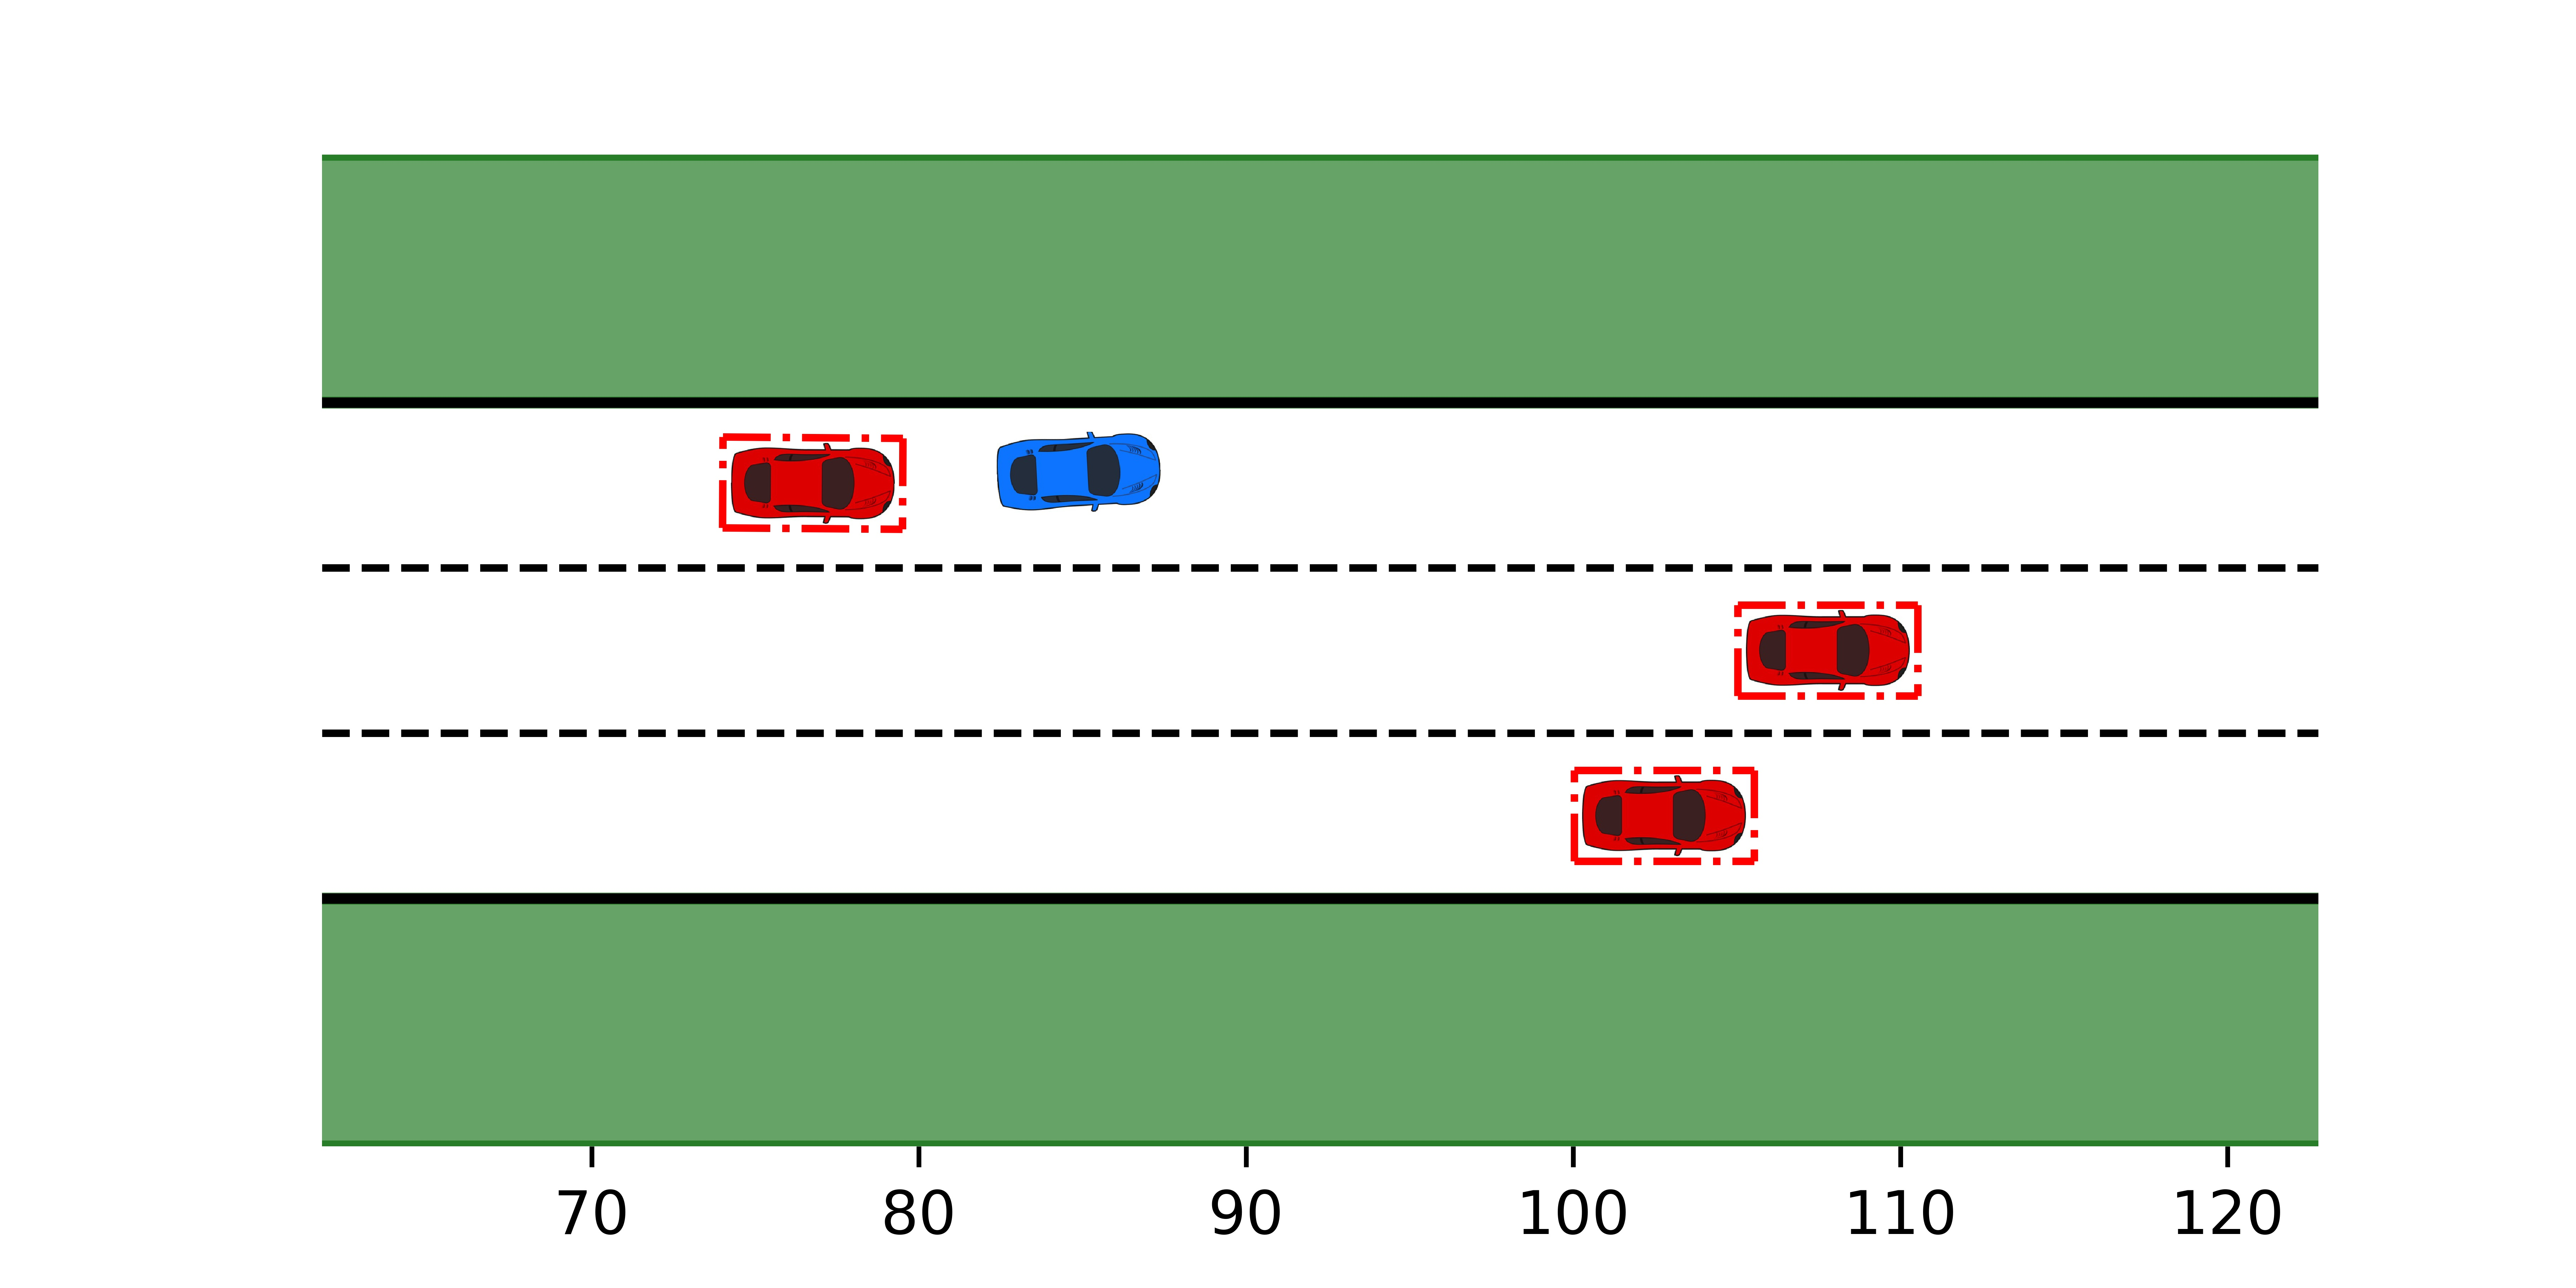
\includegraphics[clip, trim = {1.5cm 0.25cm 1.5cm 0.25cm}]{plot_agg8.jpg}};
			\node (con5)[ right = 1cm of adp5, minimum width = 0.cm, minimum height = 0cm, inner sep = 0pt]{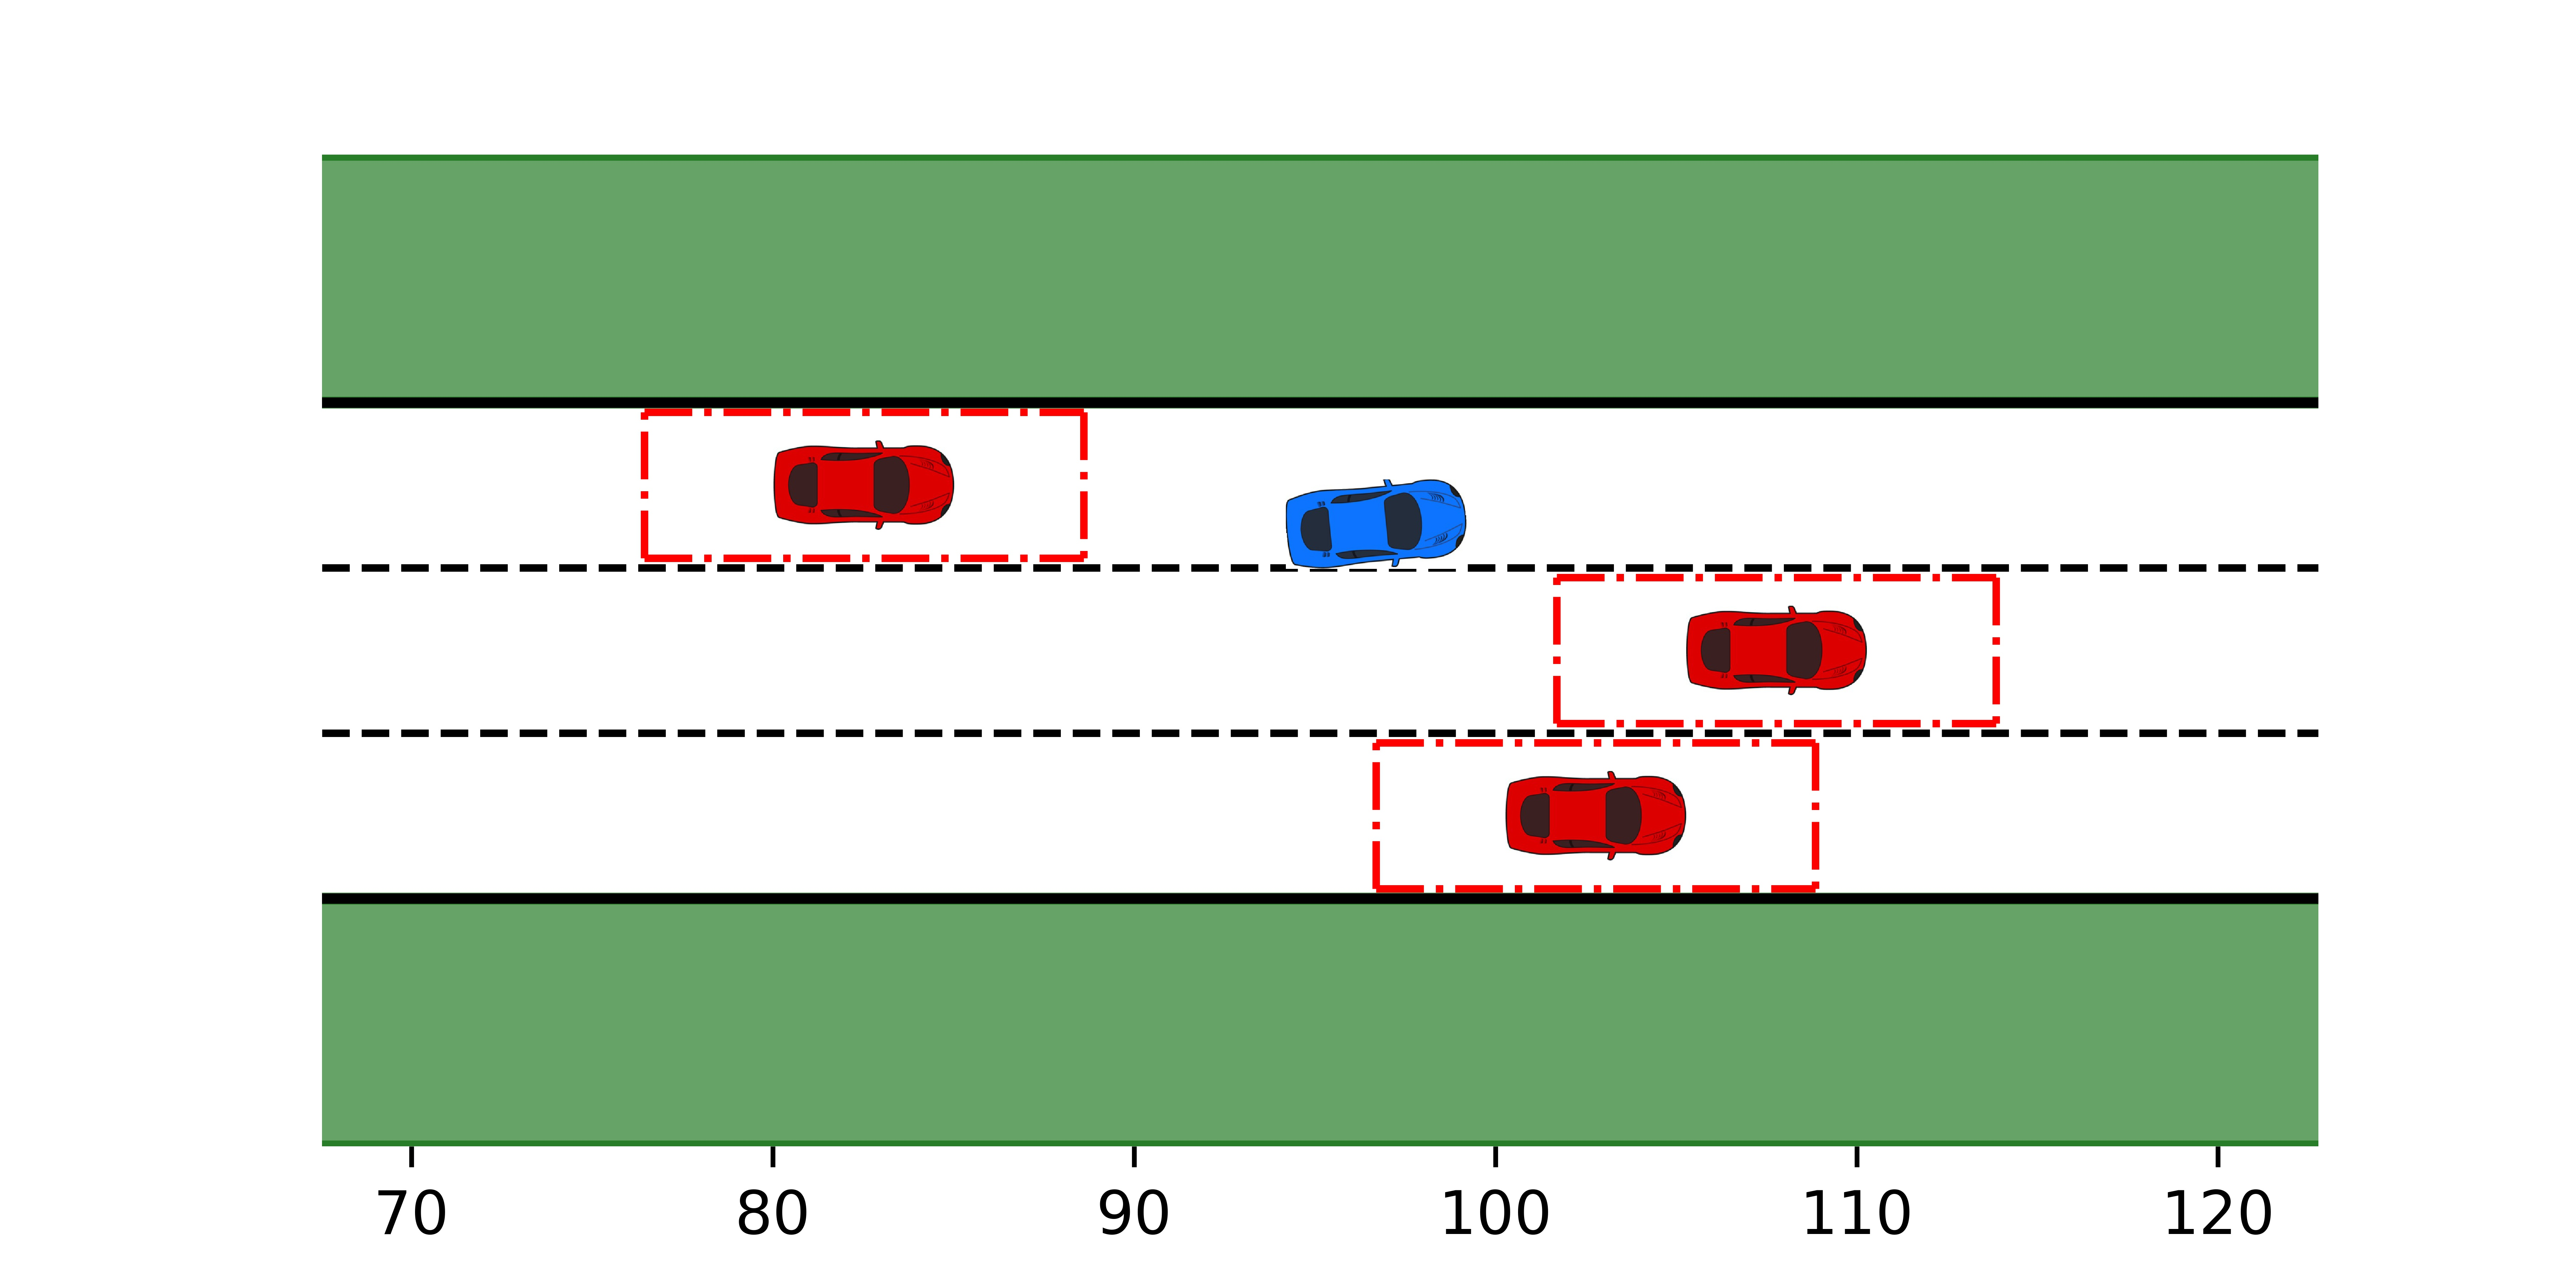
\includegraphics[clip, trim = {1.5cm 0.25cm 1.5cm 0.25cm}]{plot_con8.jpg}};
			%			
			%			\node (adp6)[below  = 1.5cm of adp5, minimum width = 0.cm, minimum height = 0cm, inner sep = 0pt]{\includegraphics[clip, trim = {1.5cm 0.25cm 1.5cm 0.25cm}]{plot_adp10.jpg}};
			%			\node (agg6)[left = 1cm of adp6, minimum width = 0.cm, minimum height = 0cm, inner sep = 0pt]{\includegraphics[clip, trim = {1.5cm 0.25cm 1.5cm 0.25cm}]{plot_agg10.jpg}};
			%			\node (con6)[ right = 1cm of adp6, minimum width = 0.cm, minimum height = 0cm, inner sep = 0pt]{\includegraphics[clip, trim = {1.5cm 0.25cm 1.5cm 0.25cm}]{plot_con10.jpg}};
			
			
			\node (xlabeladp) [below = 1cm of adp5, inner sep = 0pt] {\Huge Distance (m)};
			\node (xlabelagg) [below = 1cm of agg5, inner sep = 0pt] {\Huge Distance (m)};
			\node (xlabelcon) [below = 1cm of con5, inner sep = 0pt] {\Huge Distance (m)};

			\node(car1) [below left = -2.79cm and -6.75cm of agg1, inner sep = 0pt, draw, circle, minimum height = 0.7cm, minimum width = 0.7cm] {\LARGE 1};
			\node(car3) [below left = -3.79cm and -7.95cm of agg1, inner sep = 0pt, draw, circle, minimum height = 0.7cm, minimum width = 0.7cm] {\LARGE 3};
			\node(car2) [below left = -3.79cm and -2.45cm of agg1, inner sep = 0pt, draw, circle, minimum height = 0.7cm, minimum width = 0.7cm] {\LARGE 2};
			\node(car3) [below left = -4.79cm and -2.45cm of agg1, inner sep = 0pt, draw, circle, minimum height = 0.7cm, minimum width = 0.7cm] {\LARGE 4};

			\node(lane1) [below left = -2.76cm and -11.85cm of agg1, inner sep = 0pt] {\LARGE I};
			\node(lane1) [below left = -3.76cm and -11.95cm of agg1, inner sep = 0pt] {\LARGE II};
			\node(lane1) [below left = -4.76cm and -12.05cm of agg1, inner sep = 0pt] {\LARGE III};
			
			\node (t0) [left = 0.25cm of agg1, inner sep = 0pt] {\Huge $t=0 s$};
			\node (t1) [left = 0.25cm of agg2, inner sep = 0pt] {\Huge $t=1 s$};
			\node (t2) [left = 0.25cm of agg3, inner sep = 0pt] {\Huge $t=2 s$};
			\node (t3) [left = 0.25cm of agg4, inner sep = 0pt] {\Huge $t=3 s$};
			\node (t4) [left = 0.25cm of agg5, inner sep = 0pt] {\Huge $t=4 s$};
			
			\node (agg) [above = 0.25cm of agg1, inner sep = 0pt] {\Huge (a) Nominal};
			\node (adp) [above = 0.25cm of adp1, inner sep = 0pt] {\Huge (b) Adaptive};
			\node (con) [above = 0.25cm of con1, inner sep = 0pt] {\Huge (c) Robust};
			
			
			\end{tikzpicture}
			\par\end{centering}
		\protect\caption{A four second simulation sequence with a one second time interval (see along the column) showing the lane changing maneuver performed by the autonomous vehicle under  (a) nominal; (b) adaptive; and (c) robust decision making strategies in a multi-traffic scenario. The circled numbers indicate the vehicle ids and the Roman numerals denote the lane number in the subfigure $[1,\,1]$. The dash-dotted lines indicate the set $s \oplus \bar{\mathcal{W}}_{i}^{l}(t),\, \forall i \in \mathcal{O}$ from the perspective of the autonomous agent.}
		\label{fig:snapshots}
	\end{figure*}

	%==========================================================================%
	
	\section{Simulation results}
	\label{sec:sim_results}
	The proposed adaptive robust approach is validated for the lane changing maneuver on a numerically simulated three lane highway section\footnote{The code is made publicly available at \url{https://github.com/gokulsivasankar/RobustDecisionMaking}}. Consider the multi-agent traffic scenario shown in the subfigure $[1,\, 1]$ (first element represents row and second element represents column) in Fig. \ref{fig:snapshots}. The objective of the autonomous agent (blue) is to change from lane II to lane III, while the human agents keep their respective lane. All the human drivers are assumed to be level-1, i.e., they exhibit cautious behavior, however, it is unknown to the AV. The sampling time is set to \SI{0.5}{s} and two step prediction horizon is considered. The proposed methodology is compared to the nominal, and the robust strategies during the decision making process. 

	The traffic simulation under the nominal decision making strategy is shown in the subfigures in the first column of Fig. \ref{fig:snapshots}. In this case, the disturbance set considered for solving \eqref{eq:control_prob} is chosen as an empty set, i.e., $\bar{\mathcal{W}}_{i}^{l}(t) = \emptyset$. Since the disturbances are not considered in this case, it can be noted the AV chooses to steer left as soon as the simulation begins which provides the maximum reward. This move is considered to be aggressive. However, the human vehicle $4$, being cautious, reacts by steering left at time $t = \SI{2}{s}$ and returning to the lane center at  $t = \SI{4}{s}$ once the AV has passed. The AV completes the lane change between \SI{60}{m} and \SI{70}{m}. 

	\begin{figure}
		\begin{centering}
			\begin{tikzpicture}[scale=0.5,transform shape]
			\node (origin) at (0,0) {};
			
			\node (fig)[below left = 0cm and 0cm of origin, minimum width = 0.cm, minimum height = 0cm, inner sep = 0pt]{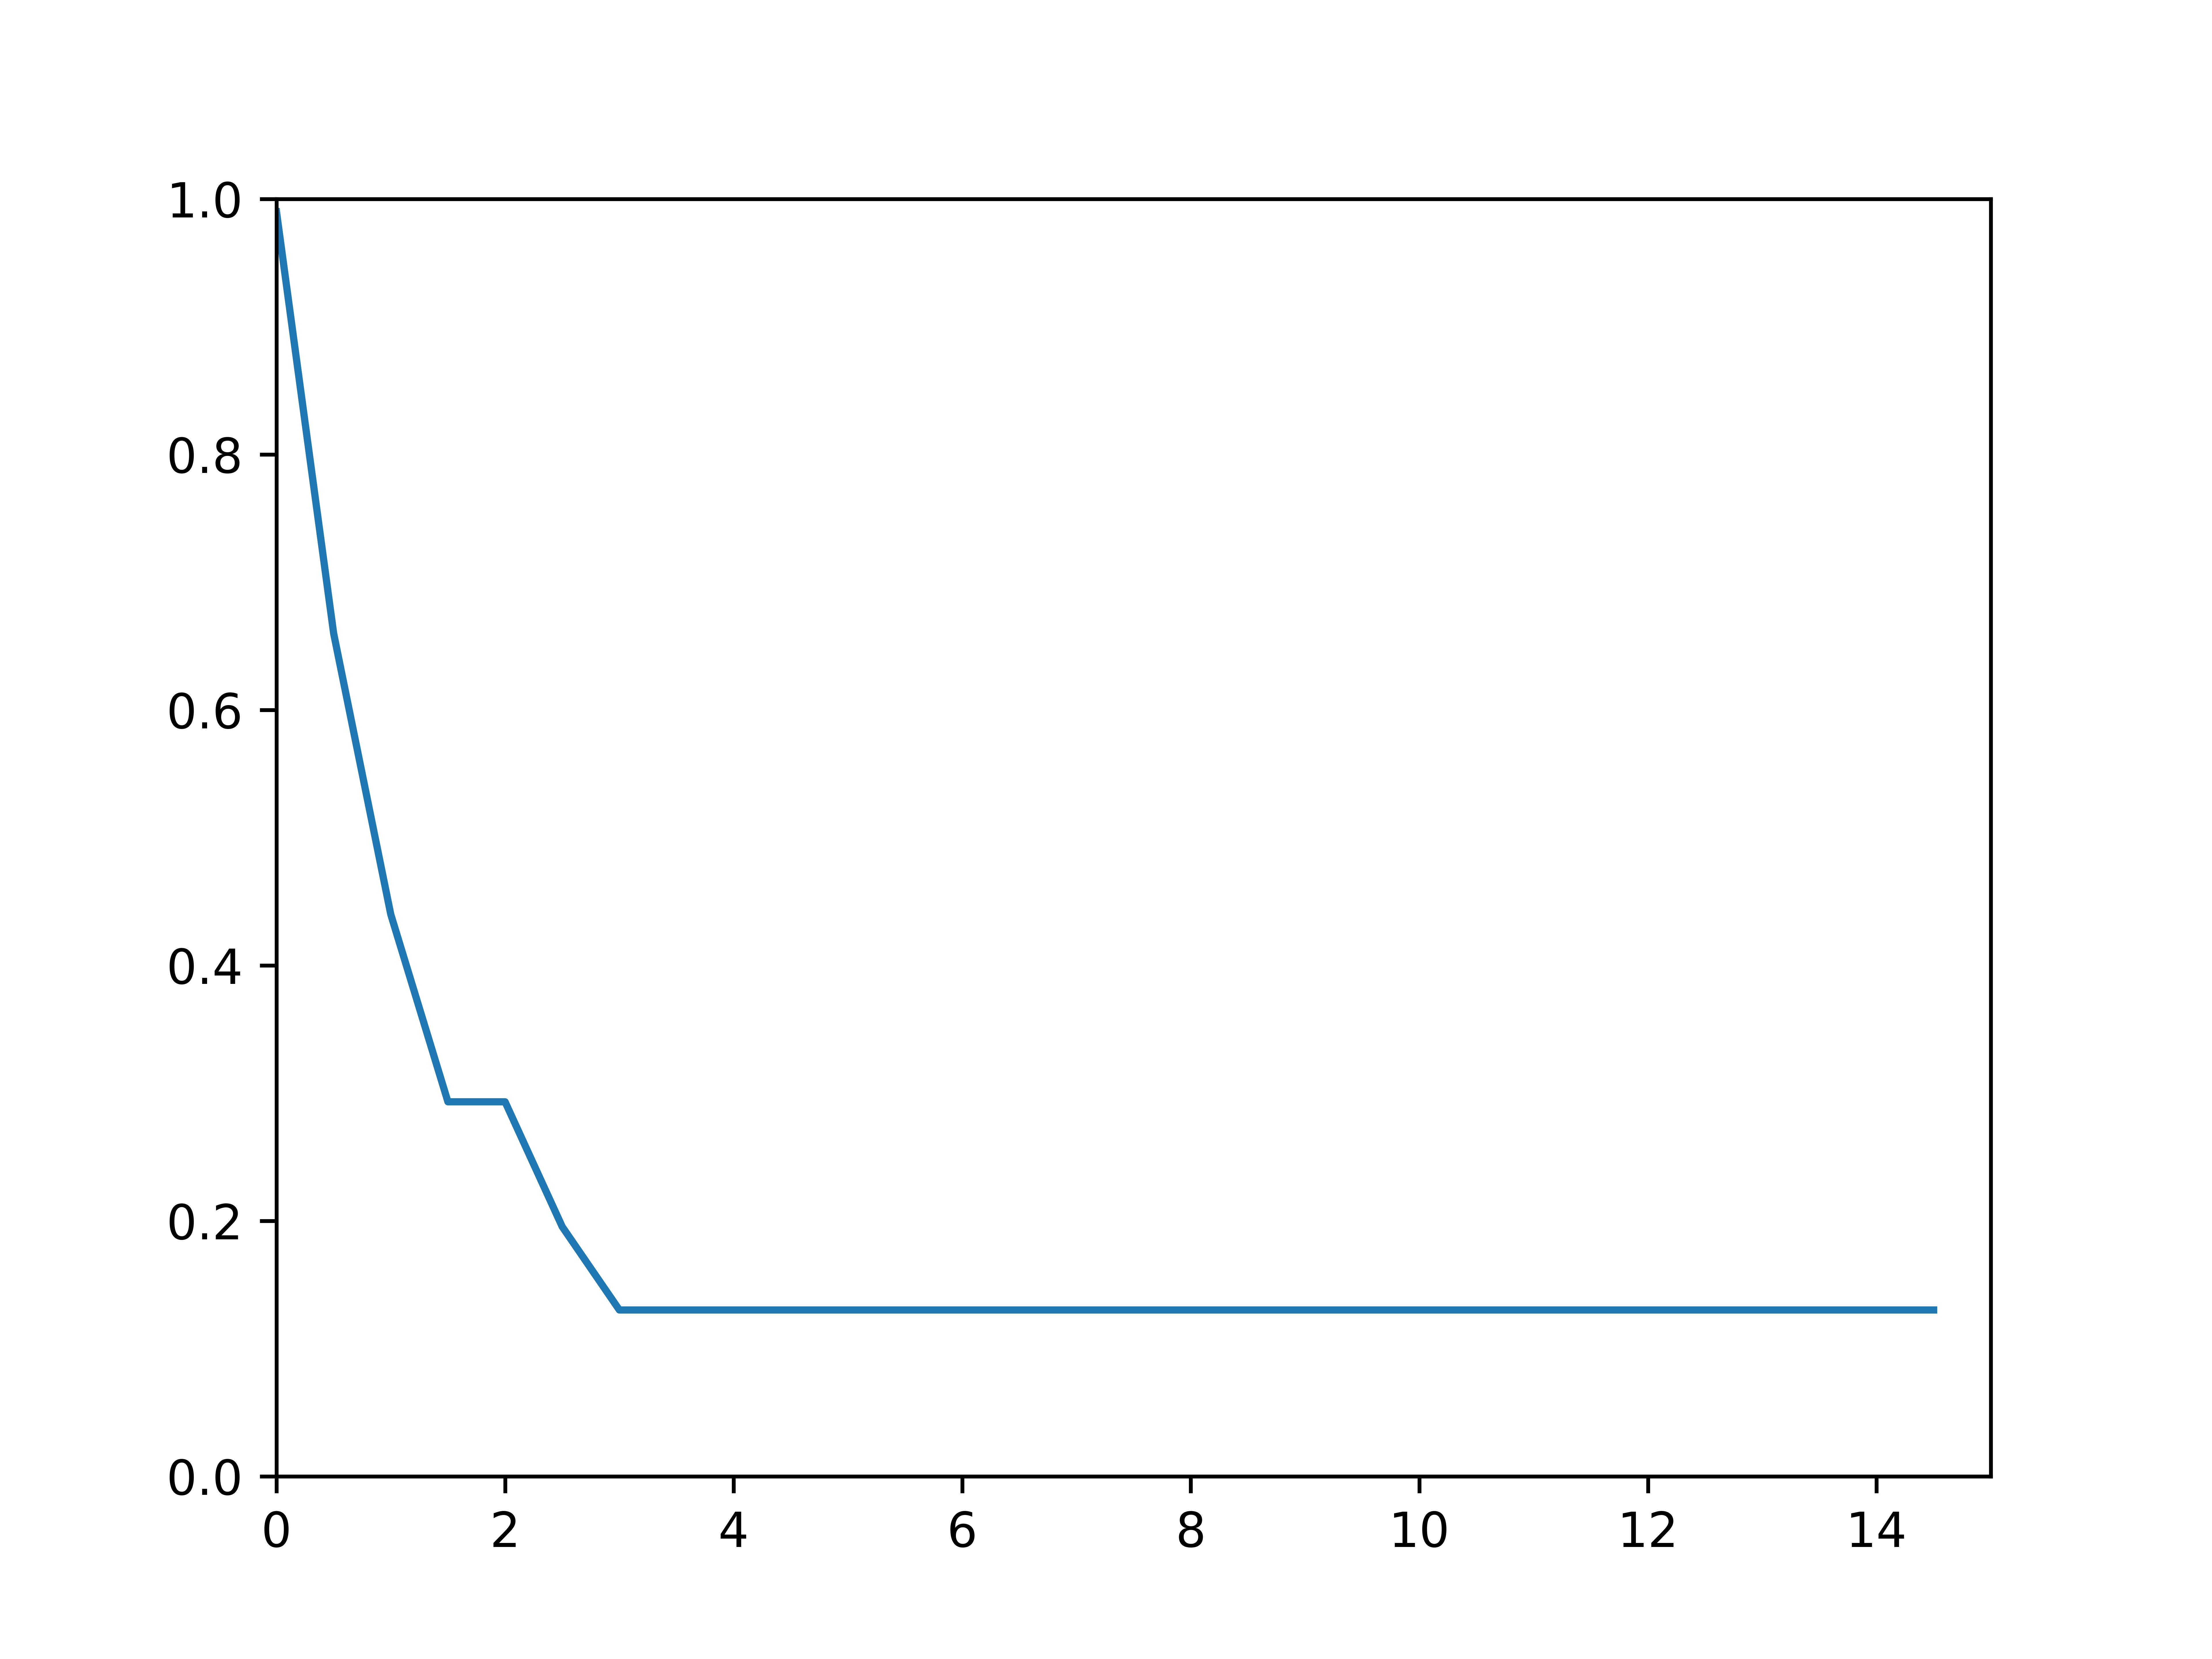
\includegraphics[clip, trim = {1.25cm 0.8cm 1.5cm 1.25cm}]{level_ratio_history_adp29.jpg}};
			
			\node (xlabel) [below = 0.5cm of fig, inner sep = 0pt] {\LARGE Time (s)};
		
			\node (ylabel) [below left = -6.1cm and 1cm of fig, inner sep = 0pt, rotate = 90] {\huge $P_{K_{4}^2 = 0}$};
			
			\end{tikzpicture}
			\par\end{centering}
		\protect\caption{Probability that the vehicle to the left of the autonomous vehicle can be modeled as level-0 from the perspective of the autonomous vehicle.}
		\label{fig:level_history}
	\end{figure}
	
	The results obtained by using the robust strategy that considers $\bar{\mathcal{W}}_{i}^{l}(t) = \mathcal{W}$, for the decision making process, is shown in the subfigures in the third column of Fig.~\ref{fig:snapshots}. The disturbance set $\mathcal{W}$ is defined as in \eqref{eq:full_dist_set}. As mentioned in Section \ref{sec:robust}, initially, all the human drivers are considered to be level-0 from the perspective of the AV, while they are assigned to be level-1 drivers. As seen in Fig.~\ref{fig:level_history}, due to interactions with vehicle $4$, as time evolves, the AV is able to reduce the probability of vehicle $4$ being level-0. It can also be noted from subfigure $[3,\,3]$ in Fig.~\ref{fig:snapshots}, robust control actions are taken to account for the set, $s \oplus \bar{\mathcal{W}}_{i}^{l}(t)$, dash-dotted box surrounding the human drivers shown in the Fig.~\ref{fig:snapshots}. As a result, the AV is conservative in performing the lane change maneuver by completing it between \SI{90}{m} and \SI{100}{m}. 
	
	Finally, the simulation results for the adaptive control strategy is shown in the subfigures in the second column of Fig.~\ref{fig:snapshots}. The initial disturbance set of all the human agents are similar to the previous case. However, by using the adaptive disturbance set in \eqref{eq:adaptive_dist_set} for computing the control actions, the AV is able to complete the lane change around \SI{70}{m}. Also, it can be observed that the size of the set, $s \oplus \bar{\mathcal{W}}_{i}^{l}(t), \, \forall i \in \{1,\,3\}$, remains constant because, the level-0 and 1 actions are the same for these two vehicles and therefore, according to \eqref{eq:model_update}, the driver model is not updated. The proposed strategy allows the AV to behave cautiously when there is uncertainty in the driver model and adapt its behavior according to the estimate of the model of the interacting driver.

	
	
	%==========================================================================%
	
	\section{Conclusions}
	\label{sec:conclusions}
	

	We proposed the robust decision-making strategy for autonomous vehicles when they share the road with the other road participants.We modeled the vehicle interactions using a level-k framework, then the decision of the autonomous vehicle was made based on the identified other vehicle's level in real-time. To avoid the conservative or aggressive behavior of autonomous vehicle, the accuracy of the level estimation was utilized to represent the uncertainty bounds of the interactive vehicles. Based on updated level estimation accuracy, the uncertainty bounds could be adjusted, and autonomous vehicle adaptively plans its motion for a given prediction horizon. Through the simulation verification, we could observe the reasonable behavior of autonomous vehicle, compared to the behaviors of conventional decision-making approaches. However, extending to handle the large number of vehicles has not been researched in this study, and computational challenge is anticipated. For the future research, we address computational tractability when the more number of interactive vehicles is given.

	%==========================================================================%

	\section*{Acknowledgement}

	We would like to express our appreciation to Mr. Nan Li and Dr. Anouck Girard who provided expertise that greatly assisted the research.



	%==========================================================================%

	\bibliographystyle{ieeetr}
	\bibliography{Reference}
	
	%	\noindent where  $t$ denotes the discrete time instant; the pair $\left(x\left(t\right),\,y\left(t\right)\right)$ $\left[\SI{}{\meter}\right]$ represent the global position of the center of mass of the vehicle; the vehicle's speed is denoted by $v\left(t\right)$ $\left[\SI{}{\meter \per \second}\right]$; 	$\beta\left(t\right)$ $\left[\SI{}{\radian}\right]$ is the angle of $v\left(t\right)$ with respect to the longitudinal axis of the vehicle; $\psi\left(t\right)$ $\left[\SI{}{\radian}\right]$ denotes the vehicle’s yaw angle (the angle between the vehicle’s heading direction and the global x-direction); $a\left(t\right)$ $\left[\SI{}{\meter \per \second^2}\right]$ denotes the vehicle’s acceleration at time $t$;  $\Delta t$ $\left[\SI{}{\second}\right]$ denotes the time step size; $\delta_f\left(t\right)$ $\left[\SI{}{\radian}\right]$ represents the front steering angle; and  $l_f$ $\left[\SI{}{\meter}\right]$ and $l_r$  $\left[\SI{}{\meter}\right]$ are the distance of the center of the mass of the vehicle to the front and rear axles, respectively; $w_x\left(k\right)$ $\left[\SI{}{\meter}\right]$  and $w_x\left(k\right)$ $\left[\SI{}{\meter}\right]$ denote the uncertainty in the position of the center of mass, respectively. It is assumed the uncertainties originate from a closed and compact disturbance set, ${\mathcal{W}} \coloneqq  \left\{ w = \left(w_x,\,w_y\right) |\zeta w\leq\theta,\,\zeta\in\mathbb{R}^{a\times 2},\,\theta\in\mathbb{R}^{b}\right\}$, with $b \in 2\mathbb{Z}^{+}$. The disturbance set is assumed to contain the origin. Furthermore, it is assumed that the rear wheels cannot be steered. The acceleration, $a\left(t\right)$, and the front steering angle, $\delta_f\left(t\right)$, are the two inputs. At a given time instant, the vehicle selects the inputs from an action set as described below.
	
\end{document}